\documentclass{beamer}

\mode<presentation>
{
  \usetheme{Antibes}
  \usecolortheme{beaver}
  % or ...

  \setbeamercovered{transparent}
  % or whatever (possibly just delete it)
}

\graphicspath{{../graphics/}}

\usepackage[english]{babel}
\usepackage[utf8]{inputenc}
\usepackage{times}
\usepackage[T1]{fontenc}
\usepackage{graphicx}
\usepackage[compatibility=false]{caption}
\usepackage{subcaption}
\usepackage{physics}
\usepackage{amsmath}
\usepackage{amssymb}

\usepackage{xcolor}
\usepackage{colortbl}
\usepackage{lmodern}

\definecolor{Gray6}{gray}{0.9}

%\usepackage{multimedia}
%\usepackage{movie9}


\newcommand{\expv}[1]{\ensuremath{\mathbb{E}[ #1]}}
\newcommand{\xs}[2]{\ensuremath{\Sigma_{#1}^{(#2)}}}
\newcommand{\intO}{\ensuremath{\int\limits_{4\pi}}}
\newcommand{\intz}{\ensuremath{\int\limits_0^1}}
\newcommand{\intf}{\ensuremath{\int\limits_{-\infty}^\infty}}
\newcommand{\intzf}{\ensuremath{\int\limits_{0}^\infty}}
\newcommand{\mlsum}[2]{\ensuremath{\sum_{\tiny\begin{array}{c}#1\end{array}}^{#2}}}

\newcommand{\raven}{\texttt{RAVEN}}

\title[Additional Results] % (optional, use only with long paper titles)
{Additional Results}

%\subtitle
%{A Term Project}

\author[Talbot] % (optional, use only with lots of authors)
{Paul W. Talbot}%\inst{1}}


\institute[University of New Mexico] % (optional, but mostly needed)
{
  %\inst{1}%
  University of New Mexico%\\
  %\inst{2}
  %Idaho National Laboratory
}

\date[Nov. 3 2016] % (optional, should be abbreviation of conference name)
{Dissertation Defense, November 3, 2016\\\vspace{10pt}\small Funded by a Laboratory Directed Research effort
at \\Idaho National Laboratory}


\subject{Uncertainty Quantification}

\pgfdeclareimage[height=0.5cm]{university-logo}{unmlogo}
%\logo{\pgfuseimage{university-logo}}
\logo{\makebox[0.95\paperwidth]{
%  
\includegraphics[height=1cm]{INL}
    \hfill
    
\includegraphics[height=0.5cm]{unmlogo}}
}

\addtobeamertemplate{navigation symbols}{}{
  \usebeamerfont{footline}%
  \usebeamercolor[fg]{footline}%
  \hspace{1em}%
  \insertframenumber/\inserttotalframenumber
}

\setbeamertemplate{itemize items}[default]
\setbeamertemplate{enumerate items}[default]

\makeatletter
\def\beamer@tocaction@only#1{\only<.(1)>{\usebeamertemplate**{#1}}}
\define@key{beamertoc}{subsectionsonly}[]{\beamer@toc@subsectionstyle{show/only}\beamer@toc@subsubsectionstyle{show/shaded/hide}}
\makeatother

\setbeamercovered{invisible}

\begin{document}
\begin{frame}
  \titlepage
\end{frame}

%%%%%%%%%%%%%%%%%%%%%%%%%
%        OUTLINE        %
%%%%%%%%%%%%%%%%%%%%%%%%%
\AtBeginSubsection[]
{\begin{frame}[shrink=20,noframenumbering]{Outline}\vspace{-20pt}
  \begin{columns}
    \begin{column}{0.1\textwidth}
    \end{column}
    \begin{column}{0.9\textwidth}
      \setcounter{tocdepth}{2}
      \tableofcontents[currentsection,currentsubsection,subsectionstyle=show/shaded/hide]%,hideothersubsections]%hideothersubsections
    \end{column}
  \end{columns}
\end{frame}
}
\section{SCgPC Results}
\subsubsection{Tensor Monomials}
\begin{frame}{SCgPC Results}{Tensor Monomials}\vspace{-20pt}
  \begin{columns}
    \begin{column}{0.6\textwidth}
      \begin{block}{Tensor Monomials}
        \[u(Y) = \prod_{n=1}^N (y_n+1)\]
      \end{block}
    \end{column}
    \begin{column}{0.4\textwidth}
        \begin{figure}[h!]
          \centering
          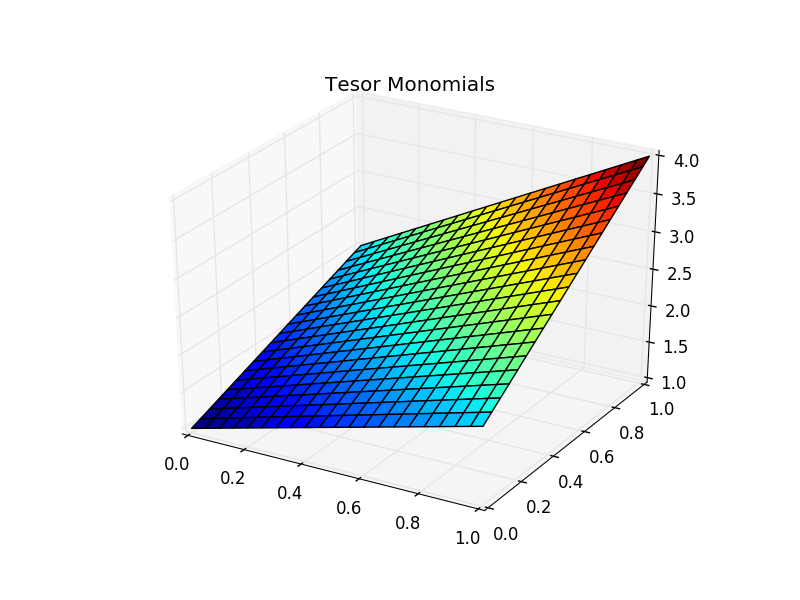
\includegraphics[width=\linewidth]{anlmodels/tensor_monom}
        \end{figure}
    \end{column}
  \end{columns}
  \begin{itemize}
    \item Linear response
    \item All polynomial combinations
  \end{itemize}
\end{frame}
\begin{frame}{SCgPC Results}{Tensor Monomials, $N=3$}\vspace{-20pt}
 \begin{columns}
   \begin{column}{0.5\textwidth}
        \begin{figure}[h!]
          \centering
          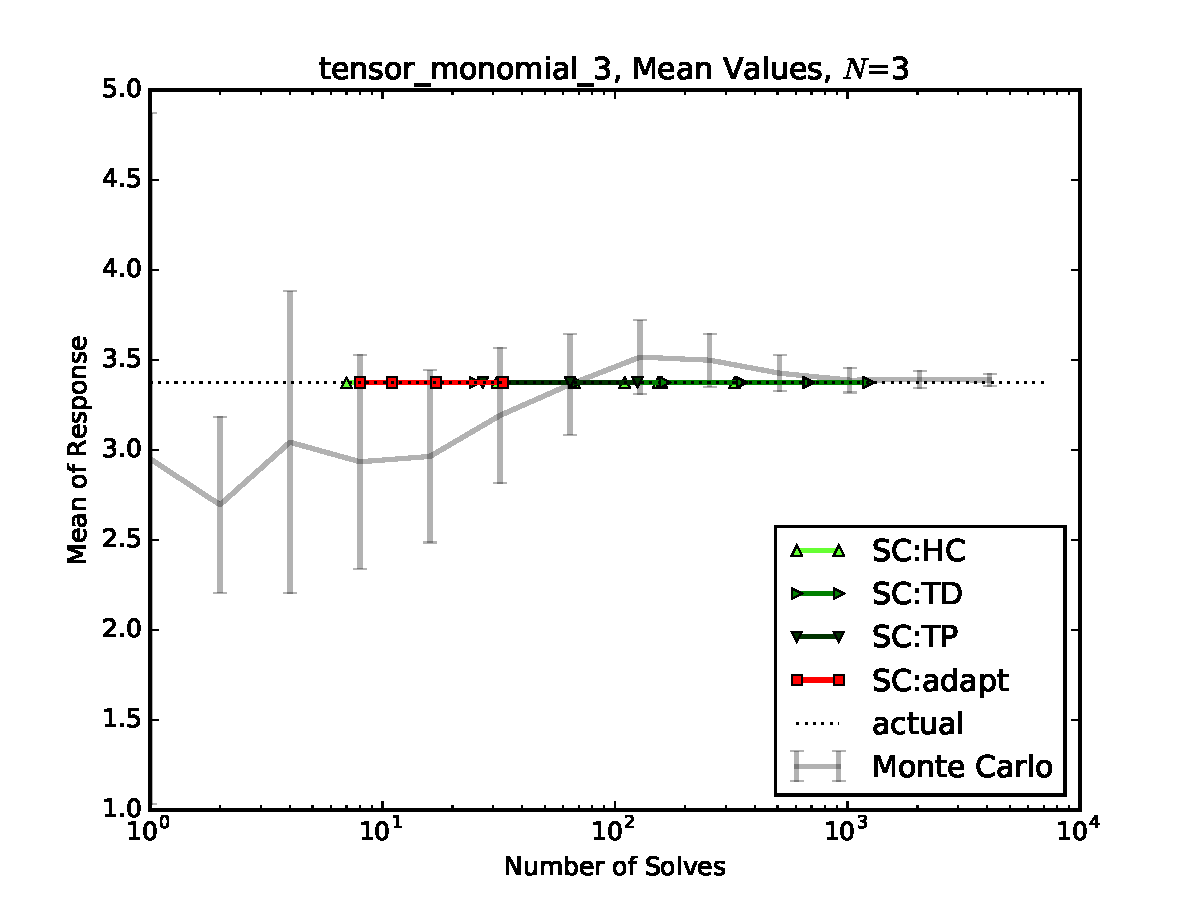
\includegraphics[width=0.8\linewidth]{anlmodels/tensor_monomial_3_mean_vals_nohdmr}
        \end{figure}
        \vspace{-20pt}
        \begin{figure}[h!]
          \centering
          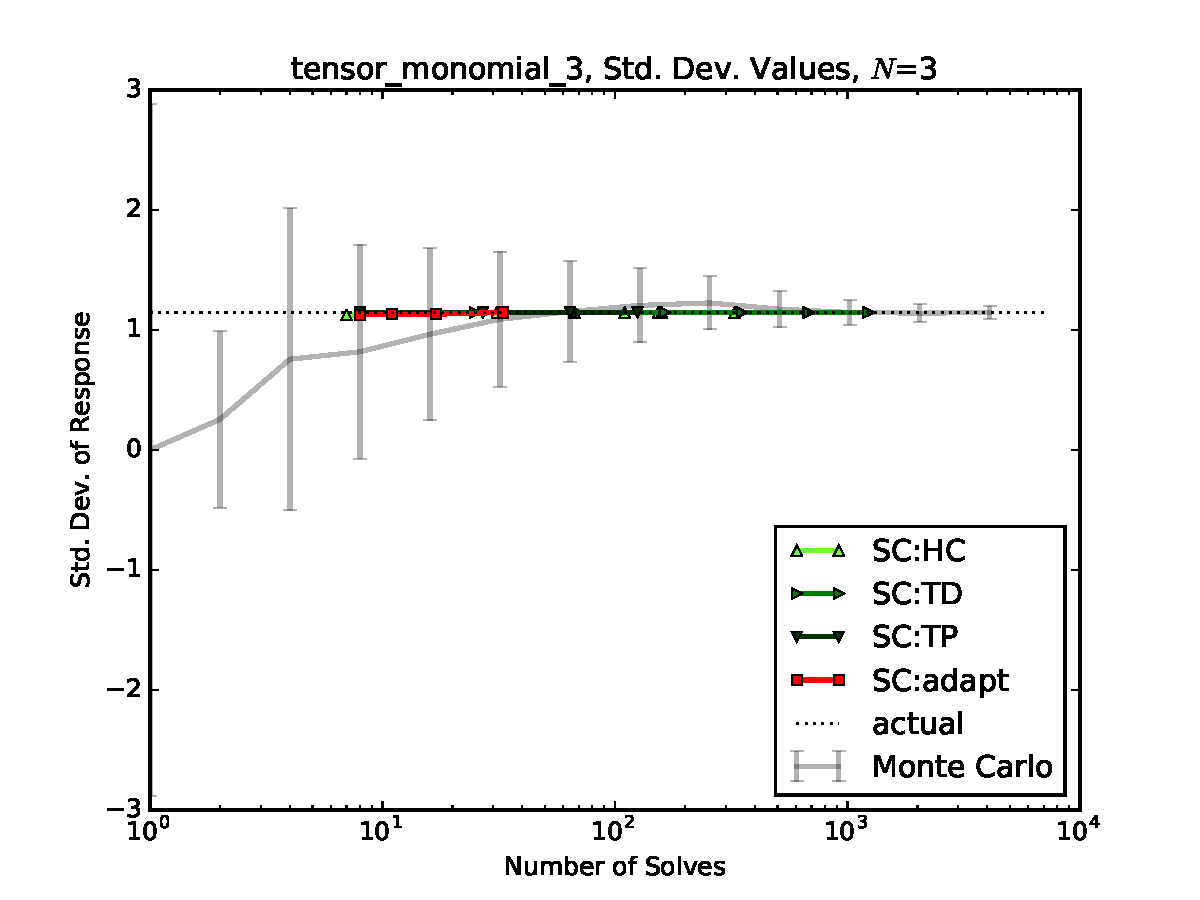
\includegraphics[width=0.8\linewidth]{anlmodels/tensor_monomial_3_var_vals_nohdmr}
        \end{figure}
   \end{column}
   \begin{column}{0.5\textwidth}
        \begin{figure}[h!]
          \centering
          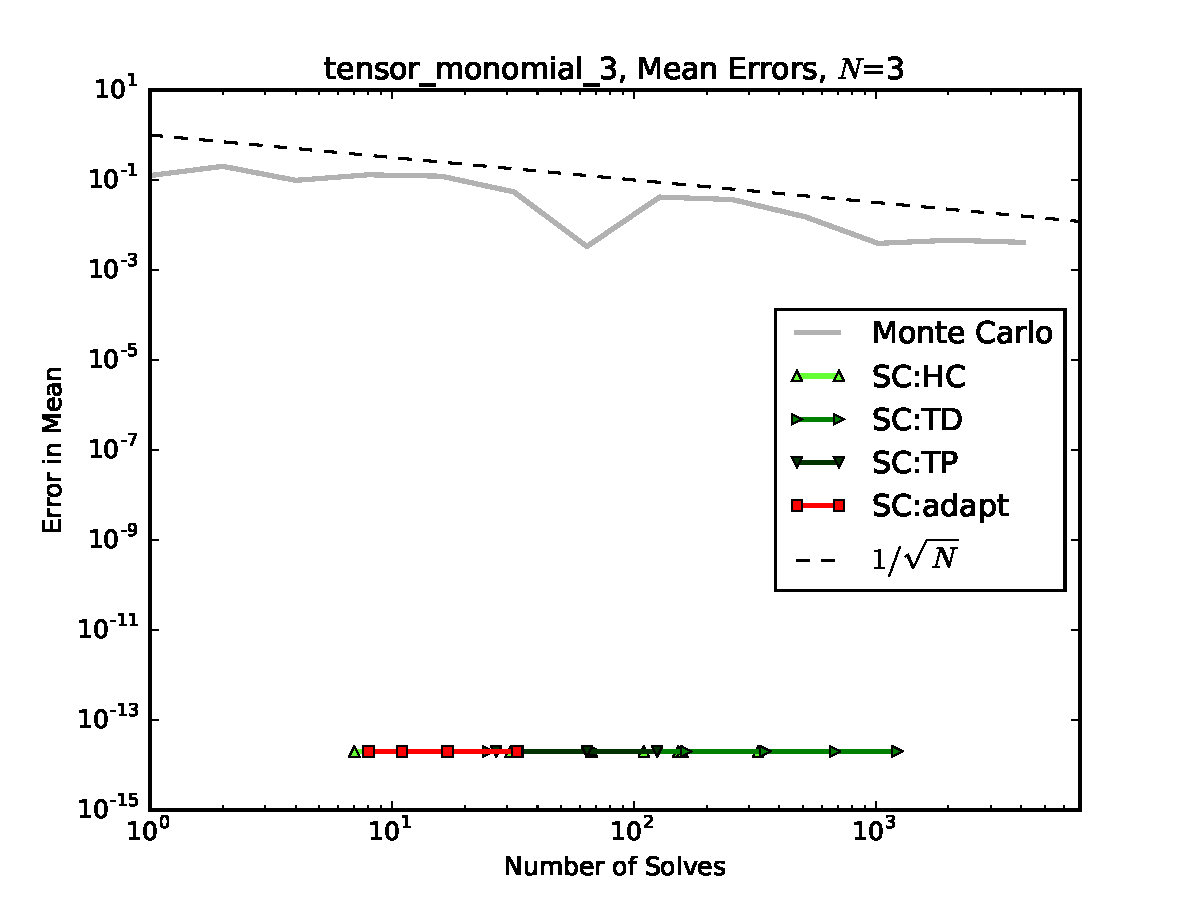
\includegraphics[width=0.8\linewidth]{anlmodels/tensor_monomial_3_mean_errs_nohdmr}
        \end{figure}
        \vspace{-20pt}
        \begin{figure}[h!]
          \centering
          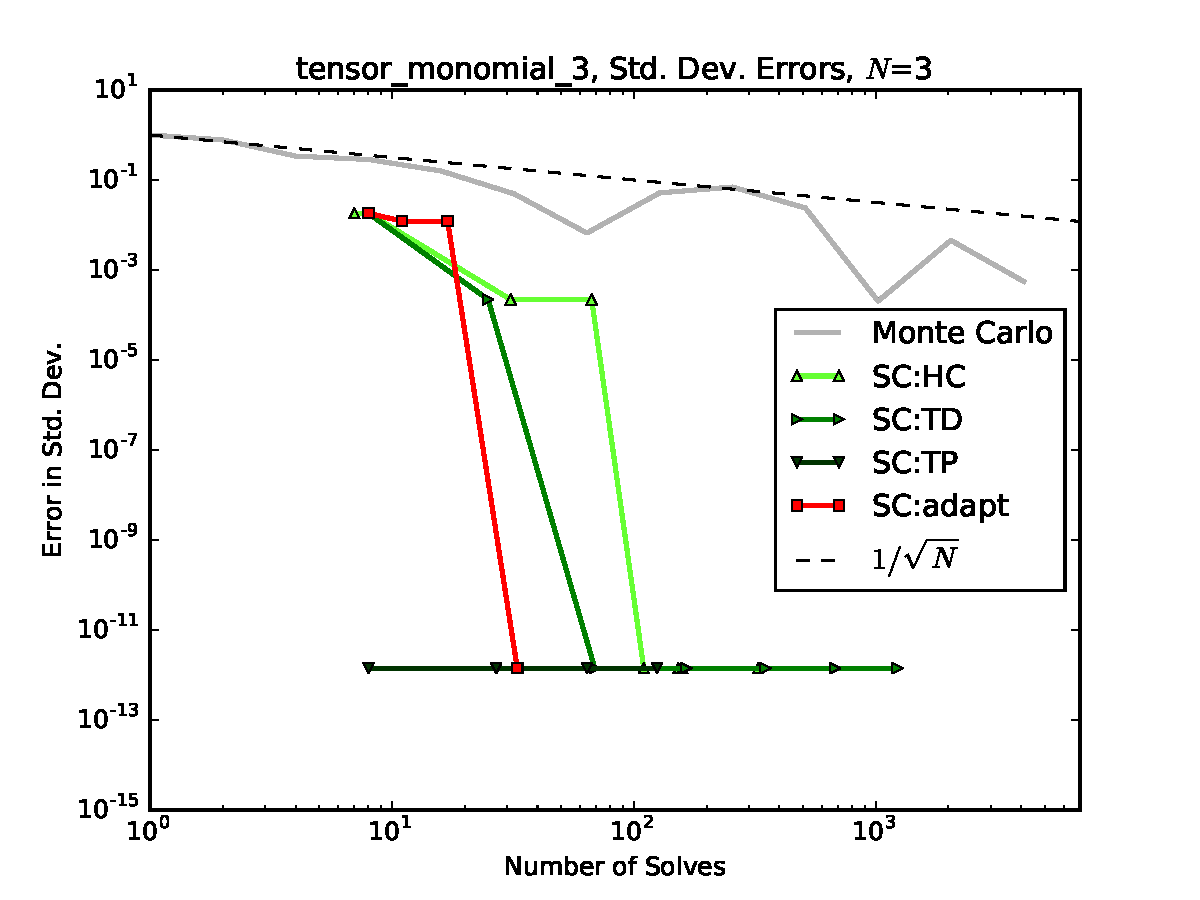
\includegraphics[width=0.8\linewidth]{anlmodels/tensor_monomial_3_variance_errs_nohdmr}
        \end{figure}
   \end{column}
 \end{columns}
\end{frame}
\begin{frame}{SCgPC Results}{Tensor Monomials, $N=5$}\vspace{-20pt}
 \begin{columns}
   \begin{column}{0.5\textwidth}
        \begin{figure}[h!]
          \centering
          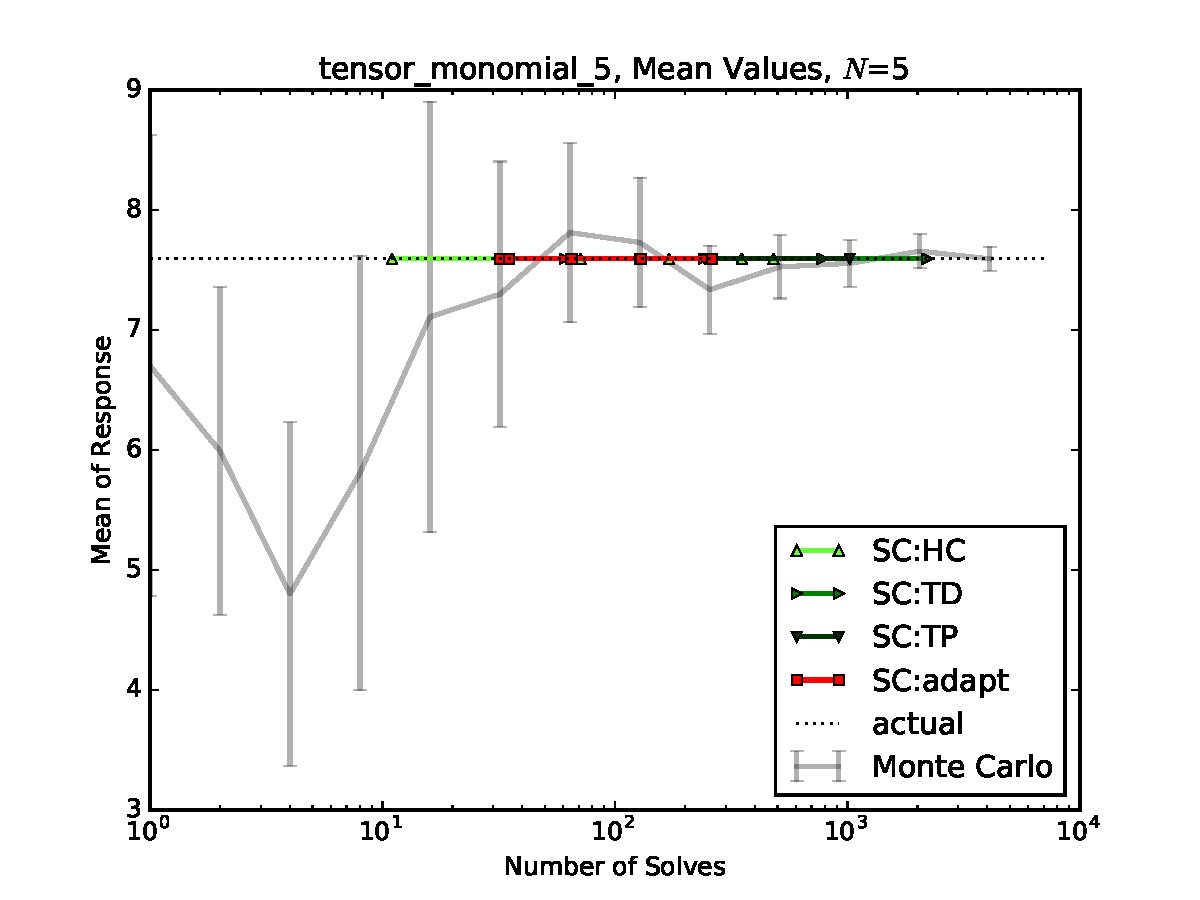
\includegraphics[width=0.8\linewidth]{anlmodels/tensor_monomial_5_mean_vals_nohdmr}
        \end{figure}
        \vspace{-20pt}
        \begin{figure}[h!]
          \centering
          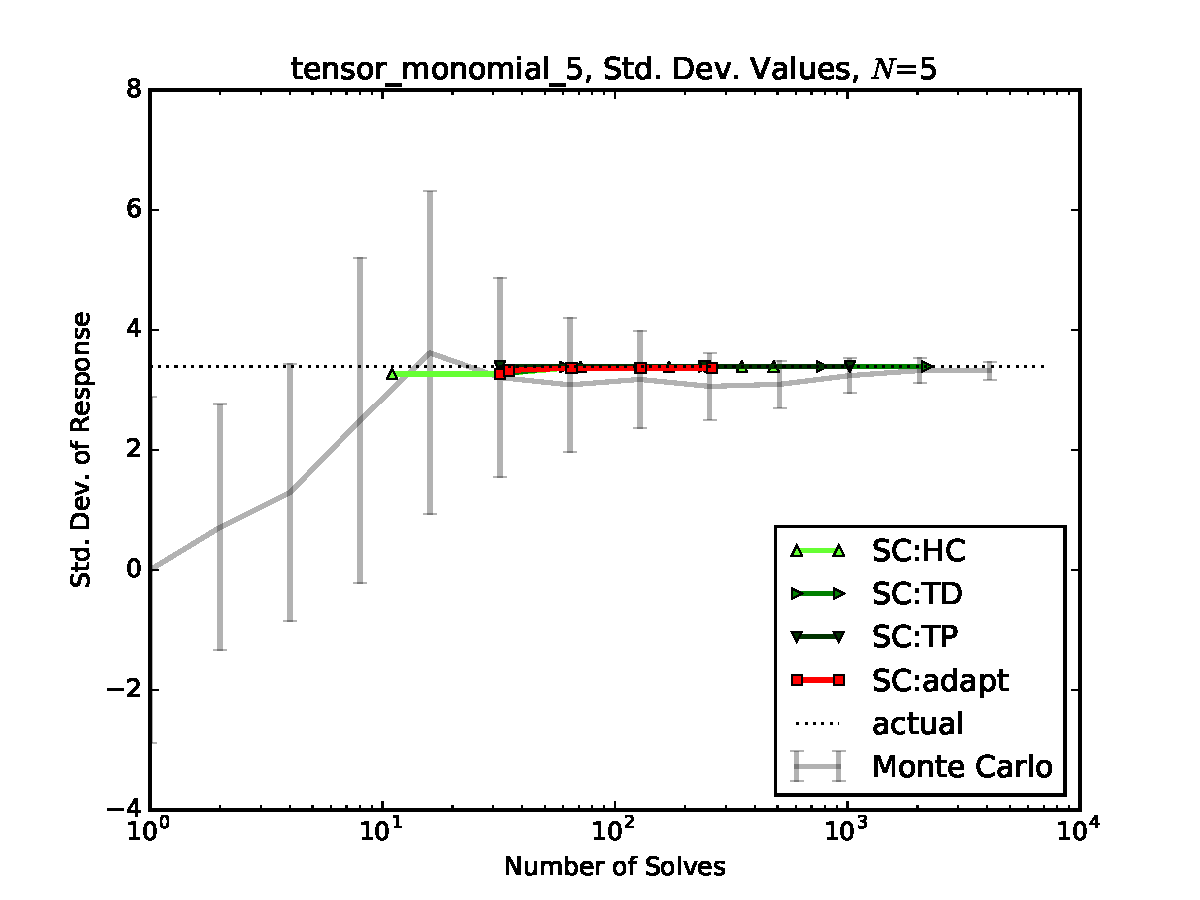
\includegraphics[width=0.8\linewidth]{anlmodels/tensor_monomial_5_var_vals_nohdmr}
        \end{figure}
   \end{column}
   \begin{column}{0.5\textwidth}
        \begin{figure}[h!]
          \centering
          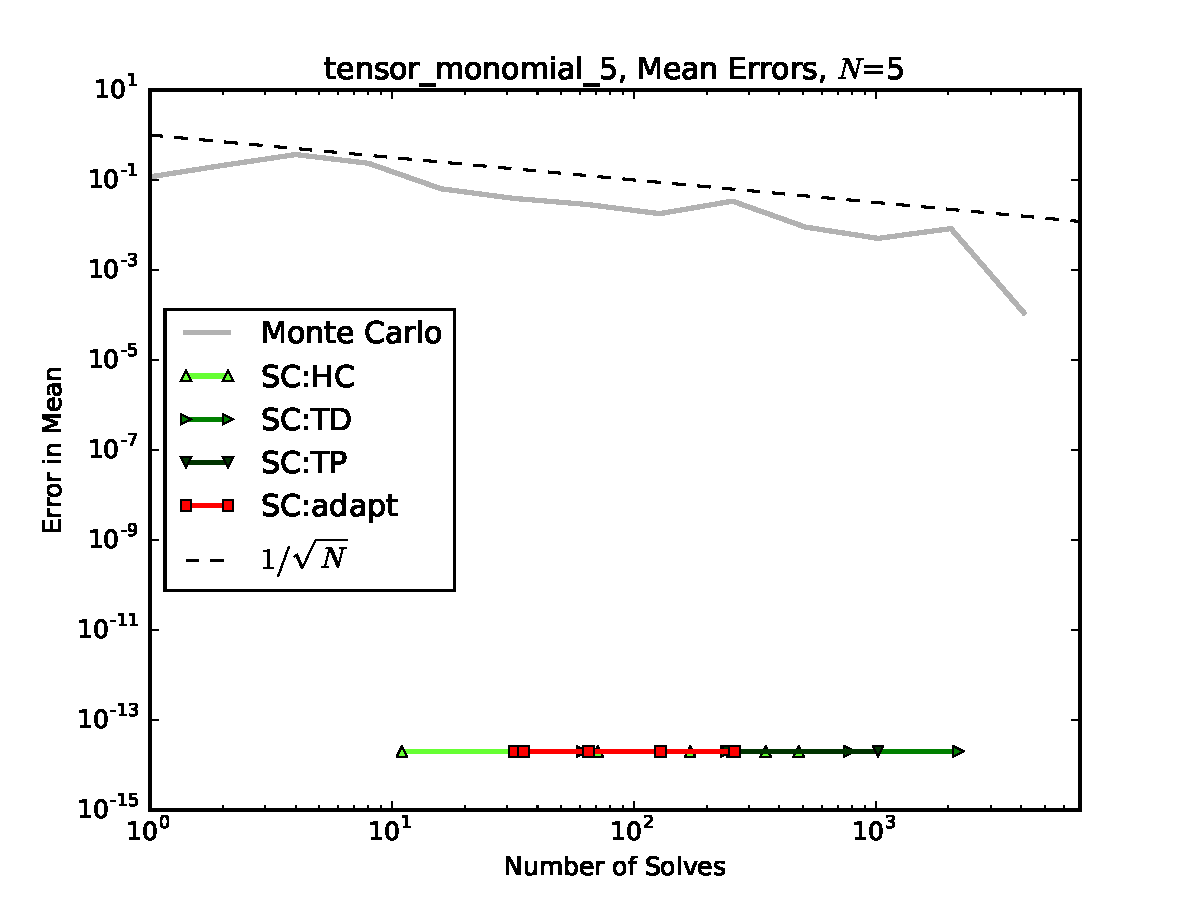
\includegraphics[width=0.8\linewidth]{anlmodels/tensor_monomial_5_mean_errs_nohdmr}
        \end{figure}
        \vspace{-20pt}
        \begin{figure}[h!]
          \centering
          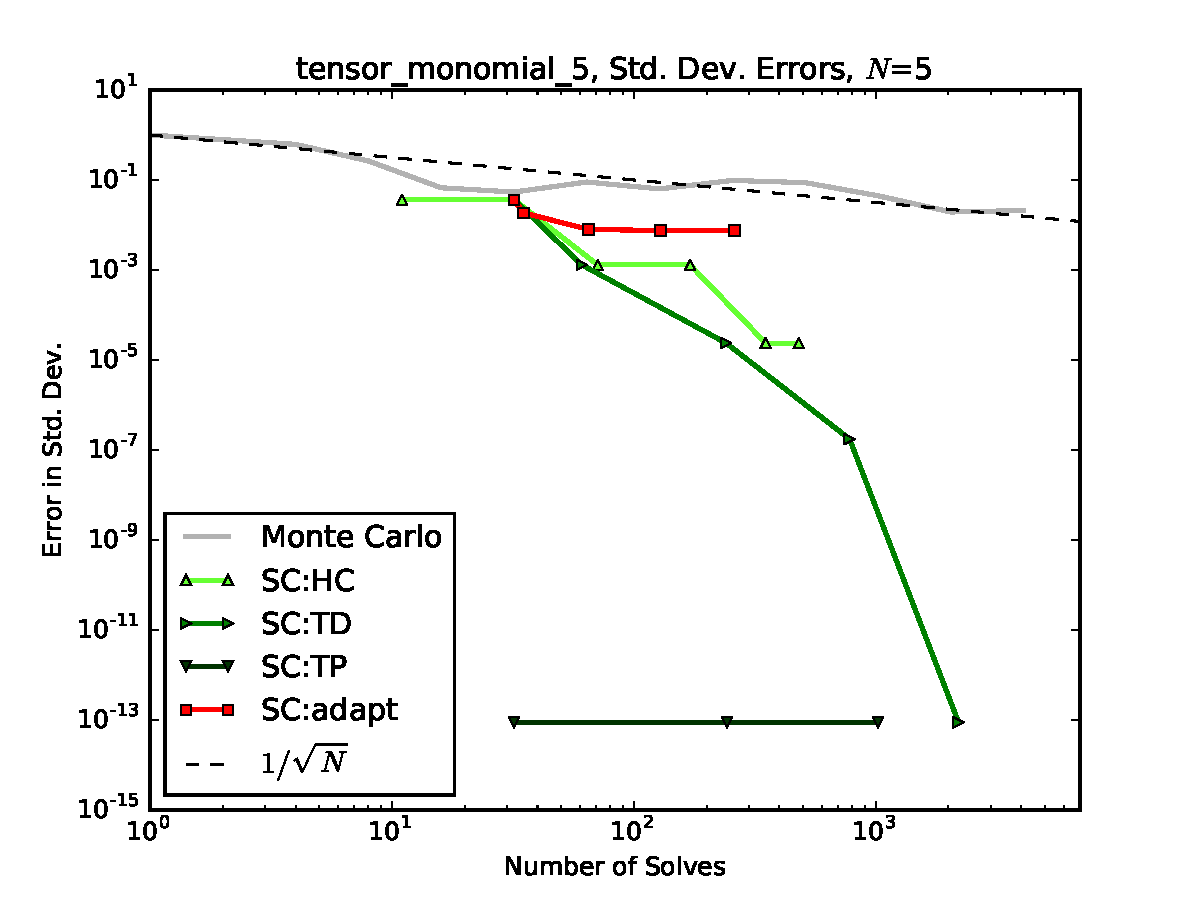
\includegraphics[width=0.8\linewidth]{anlmodels/tensor_monomial_5_variance_errs_nohdmr}
        \end{figure}
   \end{column}
 \end{columns}
\end{frame}
\begin{frame}{SCgPC Results}{Tensor Monomials, $N=10$}\vspace{-20pt}
 \begin{columns}
   \begin{column}{0.5\textwidth}
        \begin{figure}[h!]
          \centering
          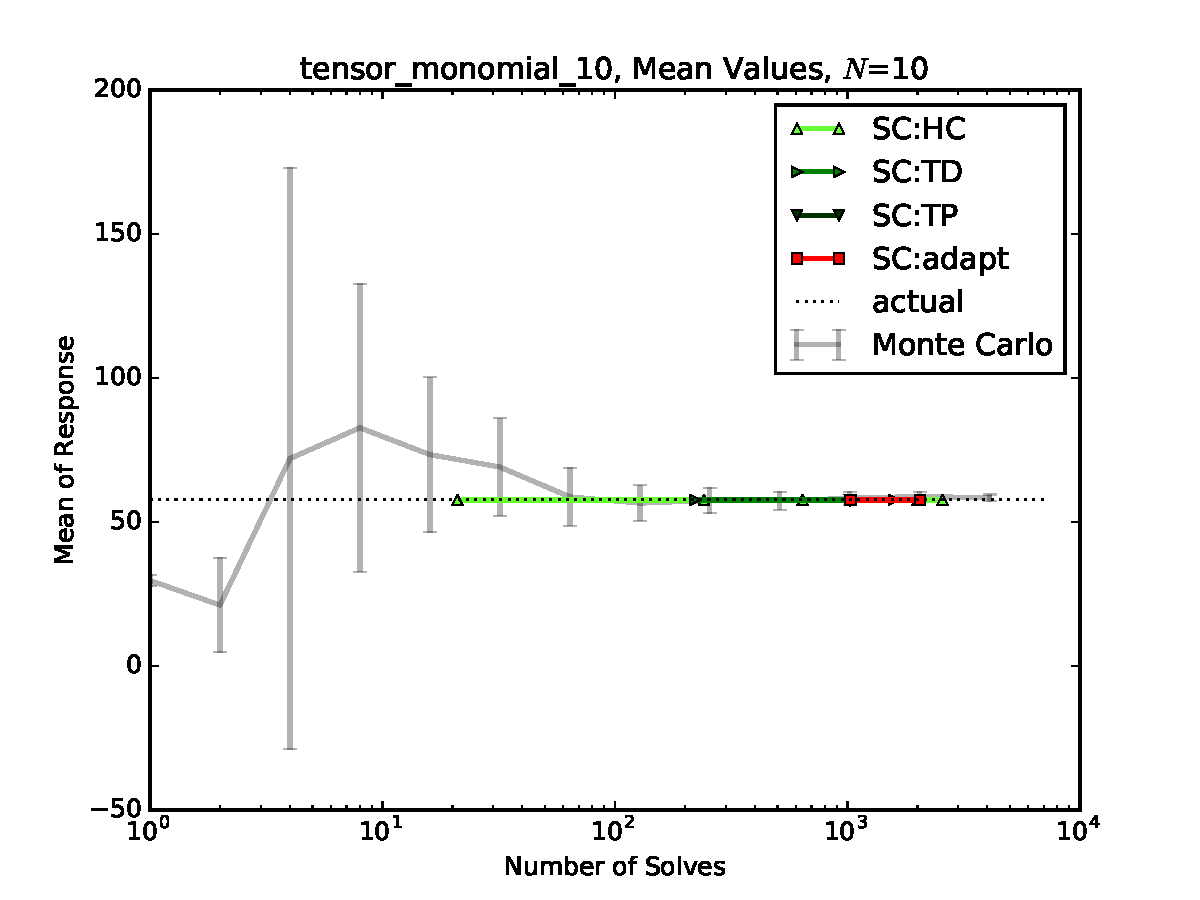
\includegraphics[width=0.8\linewidth]{anlmodels/tensor_monomial_10_mean_vals_nohdmr}
        \end{figure}
        \vspace{-20pt}
        \begin{figure}[h!]
          \centering
          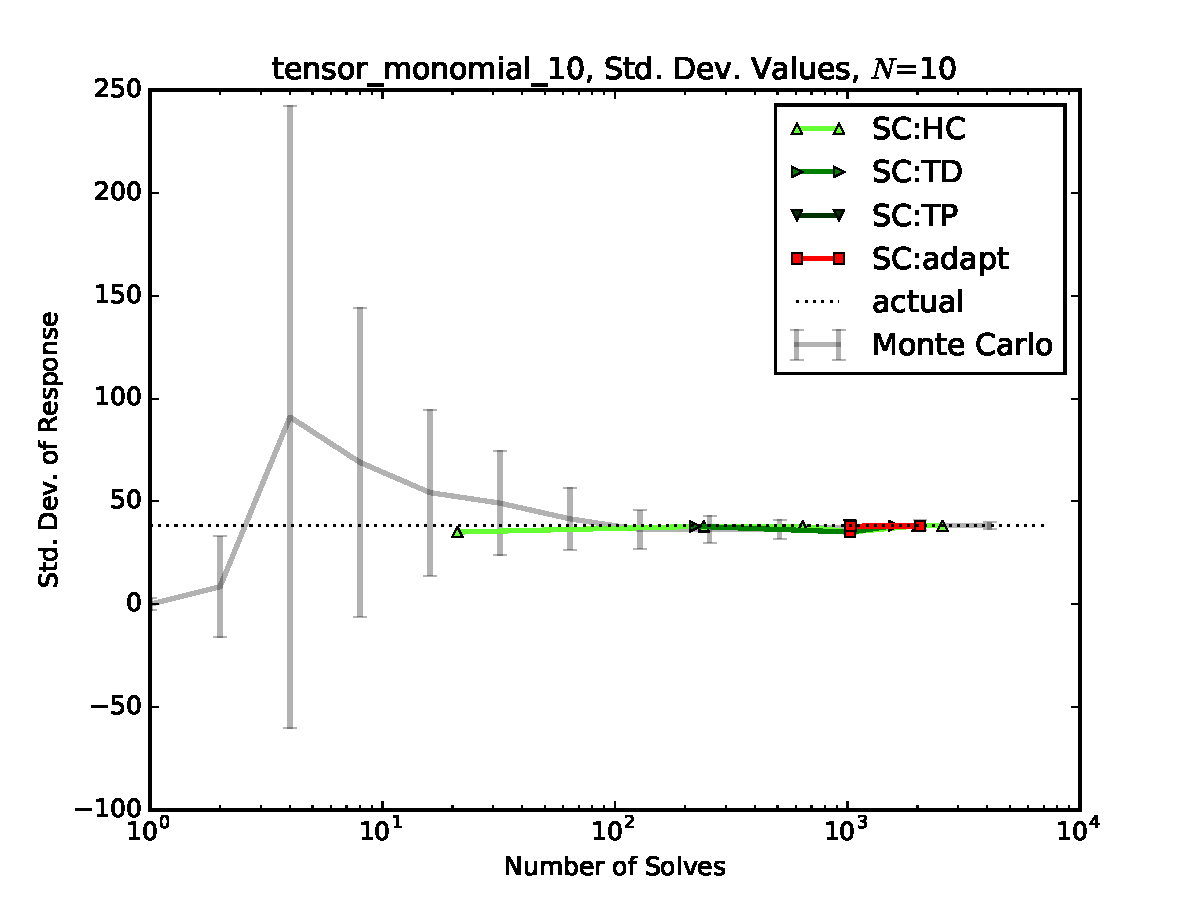
\includegraphics[width=0.8\linewidth]{anlmodels/tensor_monomial_10_var_vals_nohdmr}
        \end{figure}
   \end{column}
   \begin{column}{0.5\textwidth}
        \begin{figure}[h!]
          \centering
          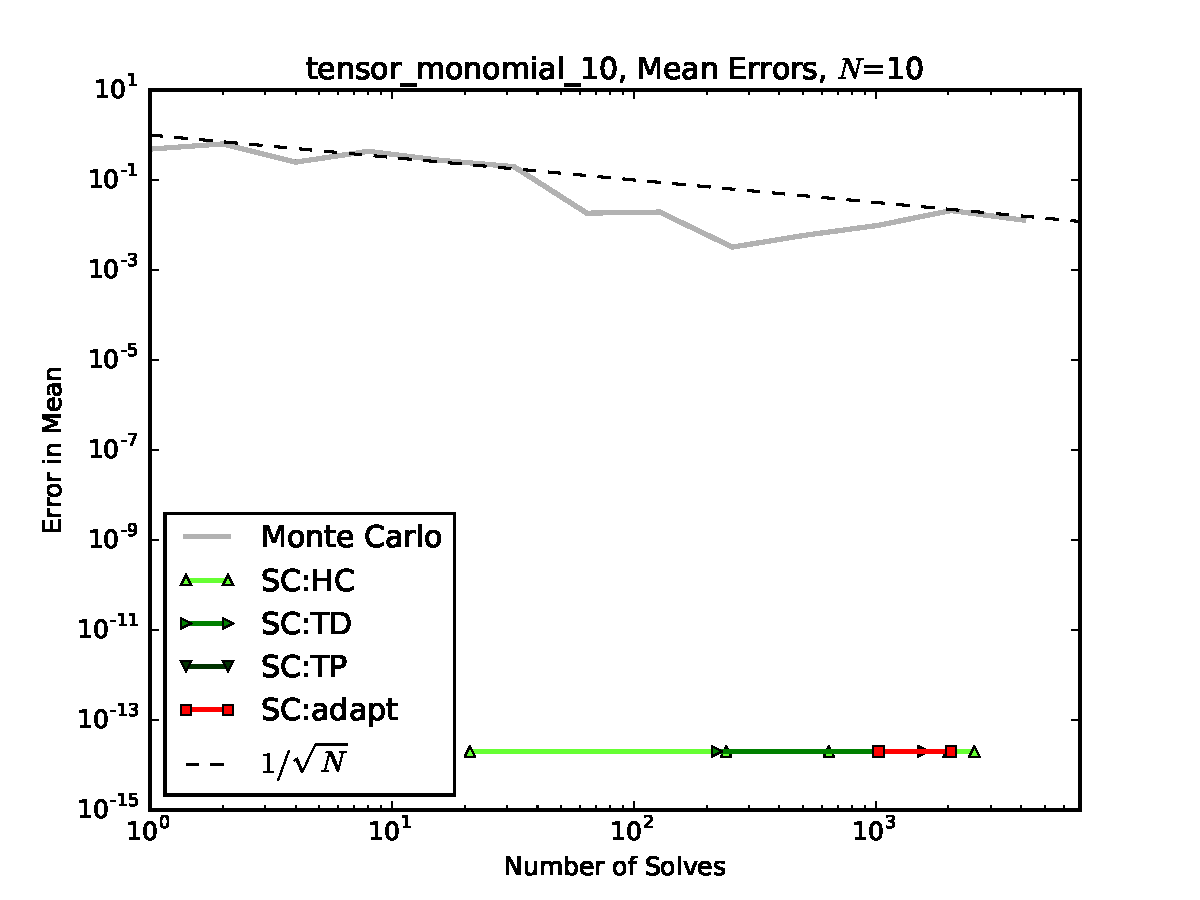
\includegraphics[width=0.8\linewidth]{anlmodels/tensor_monomial_10_mean_errs_nohdmr}
        \end{figure}
        \vspace{-20pt}
        \begin{figure}[h!]
          \centering
          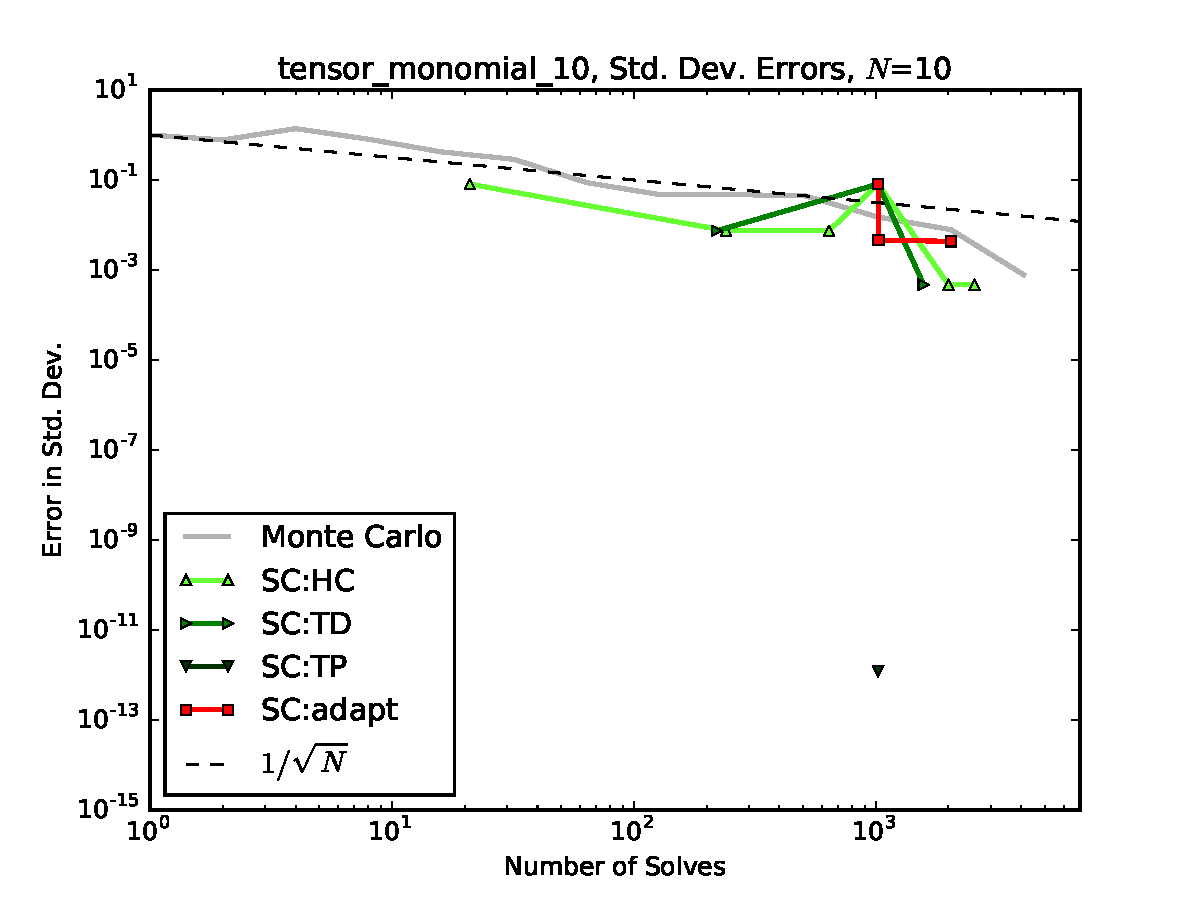
\includegraphics[width=0.8\linewidth]{anlmodels/tensor_monomial_10_variance_errs_nohdmr}
        \end{figure}
   \end{column}
 \end{columns}
\end{frame}



\subsubsection{Sudret Polynomial}
\begin{frame}{SCgPC Results}{Sudret Polynomials}\vspace{-20pt}
  \begin{columns}
    \begin{column}{0.6\textwidth}
      \begin{block}{Sudret Polynomials}
        \[u(Y) = \frac{1}{2^N}\prod_{n=1}^N (3y_n^2+1)\]
      \end{block}
    \end{column}
    \begin{column}{0.4\textwidth}
        \begin{figure}[h!]
          \centering
          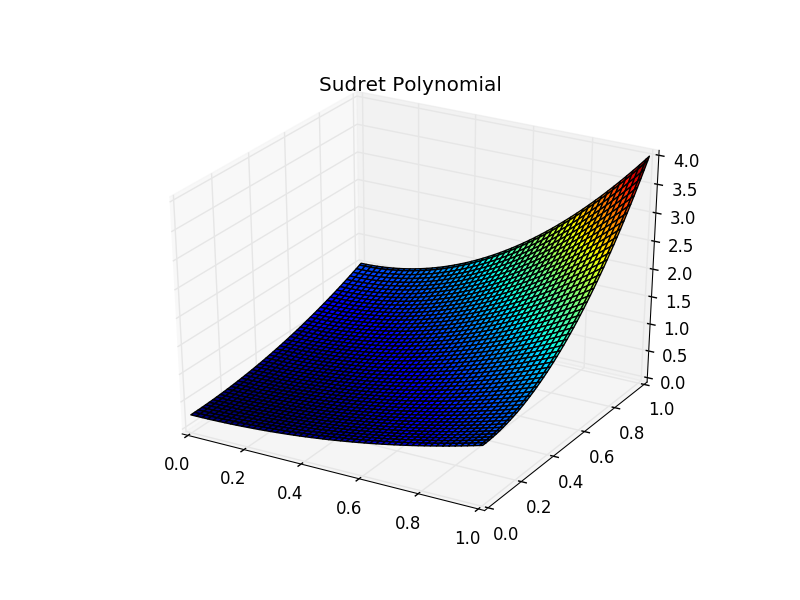
\includegraphics[width=\linewidth]{anlmodels/sudret}
        \end{figure}
    \end{column}
  \end{columns}
  \begin{itemize}
    \item Exclusively second-order interactions
    \item All second-order polynomial combinations
  \end{itemize}
\end{frame}
\begin{frame}{SCgPC Results}{Sudret Polynomials, $N=3$}\vspace{-20pt}
 \begin{columns}
   \begin{column}{0.5\textwidth}
        \begin{figure}[h!]
          \centering
          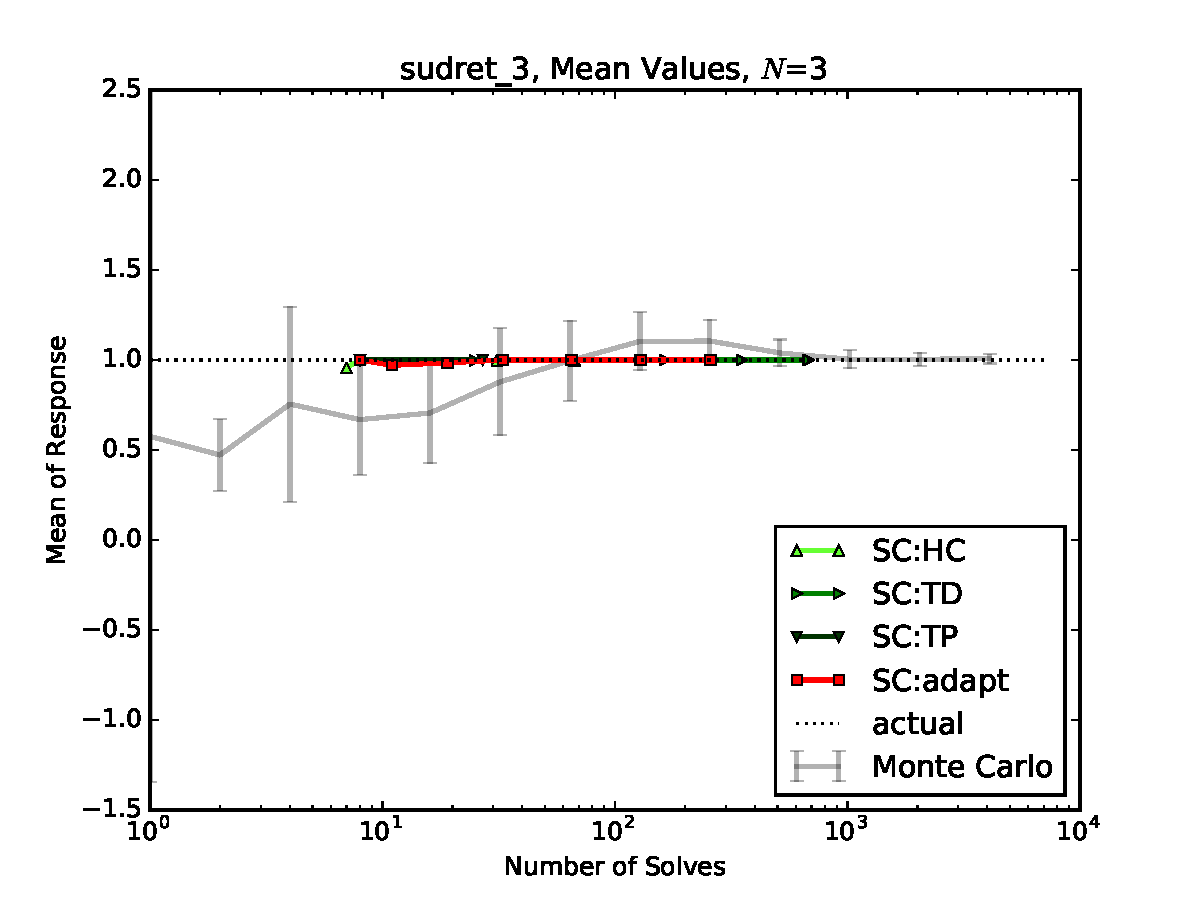
\includegraphics[width=0.8\linewidth]{anlmodels/sudret_3_mean_vals_nohdmr}
        \end{figure}
        \vspace{-20pt}
        \begin{figure}[h!]
          \centering
          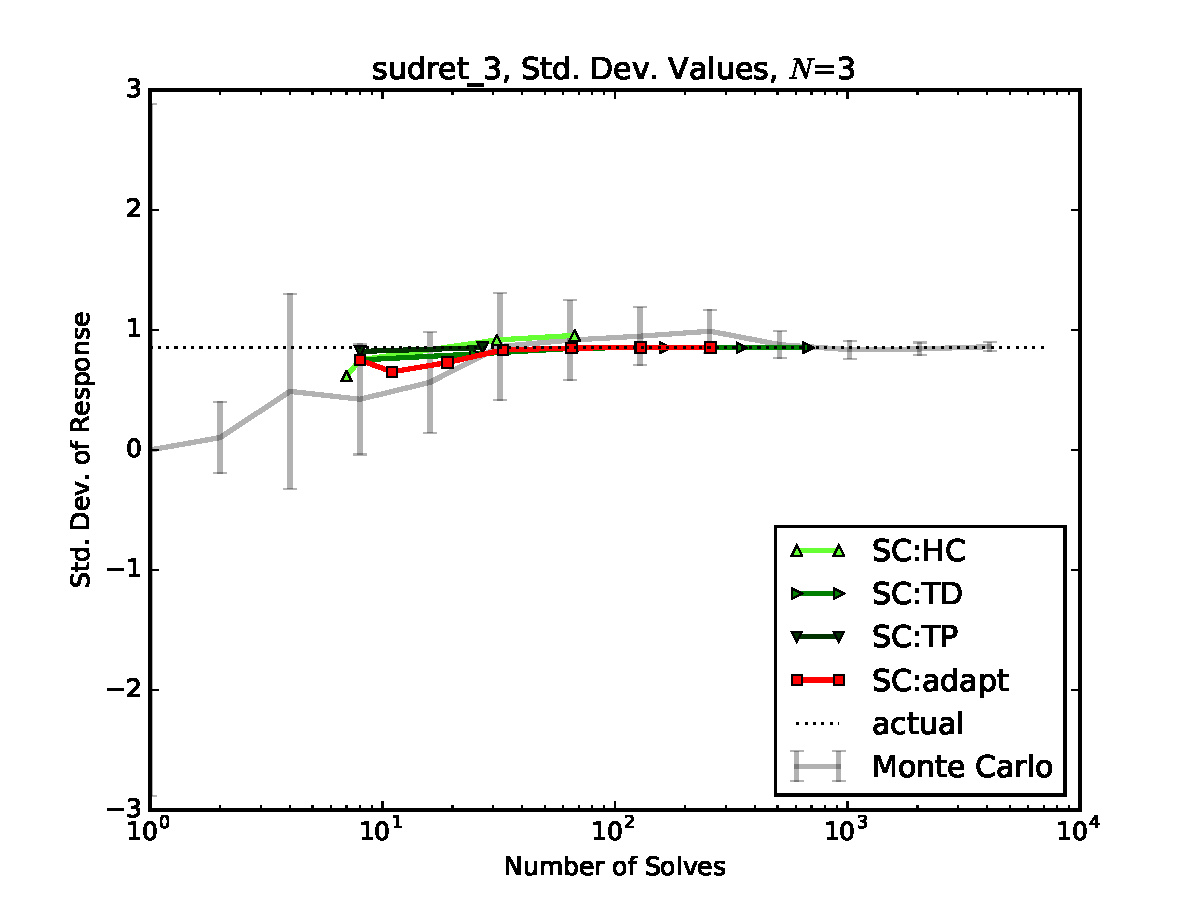
\includegraphics[width=0.8\linewidth]{anlmodels/sudret_3_var_vals_nohdmr}
        \end{figure}
   \end{column}
   \begin{column}{0.5\textwidth}
        \begin{figure}[h!]
          \centering
          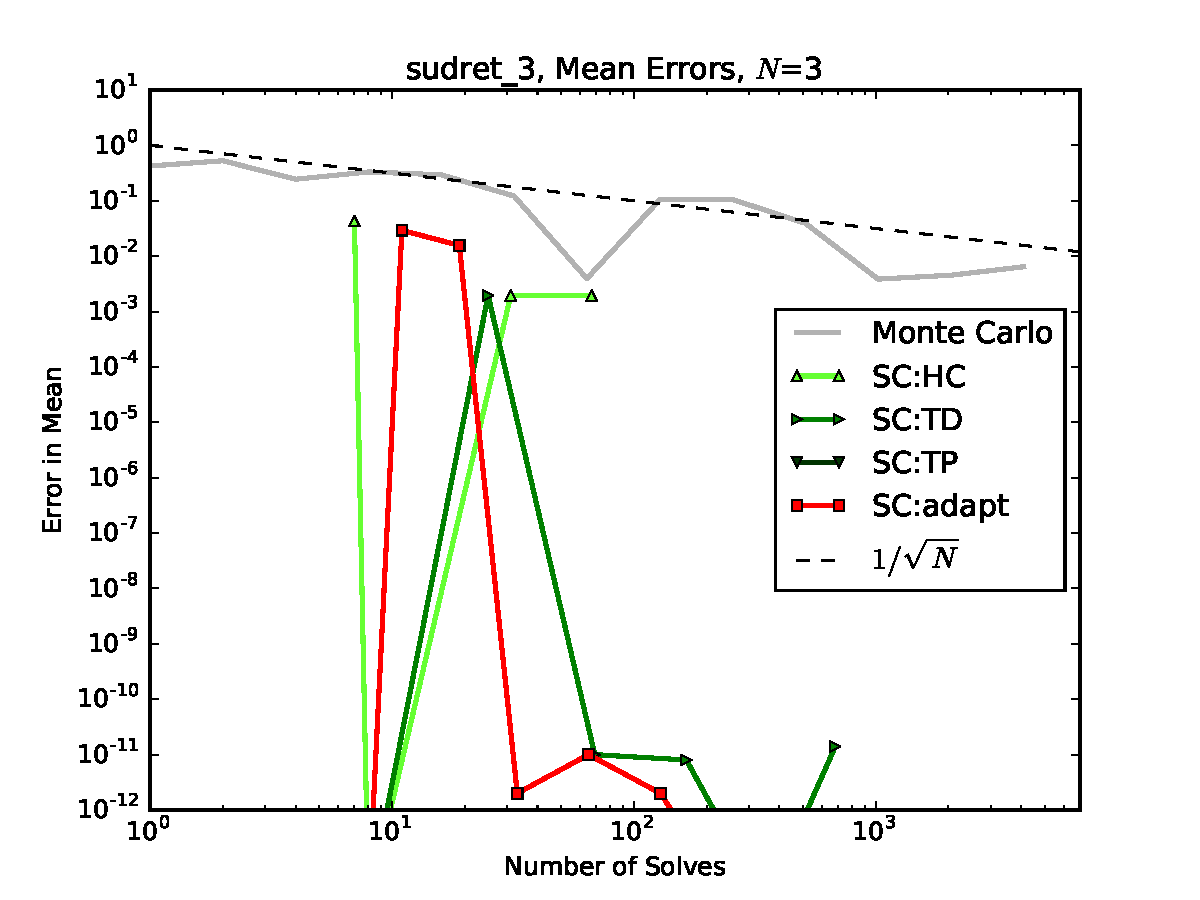
\includegraphics[width=0.8\linewidth]{anlmodels/sudret_3_mean_errs_nohdmr}
        \end{figure}
        \vspace{-20pt}
        \begin{figure}[h!]
          \centering
          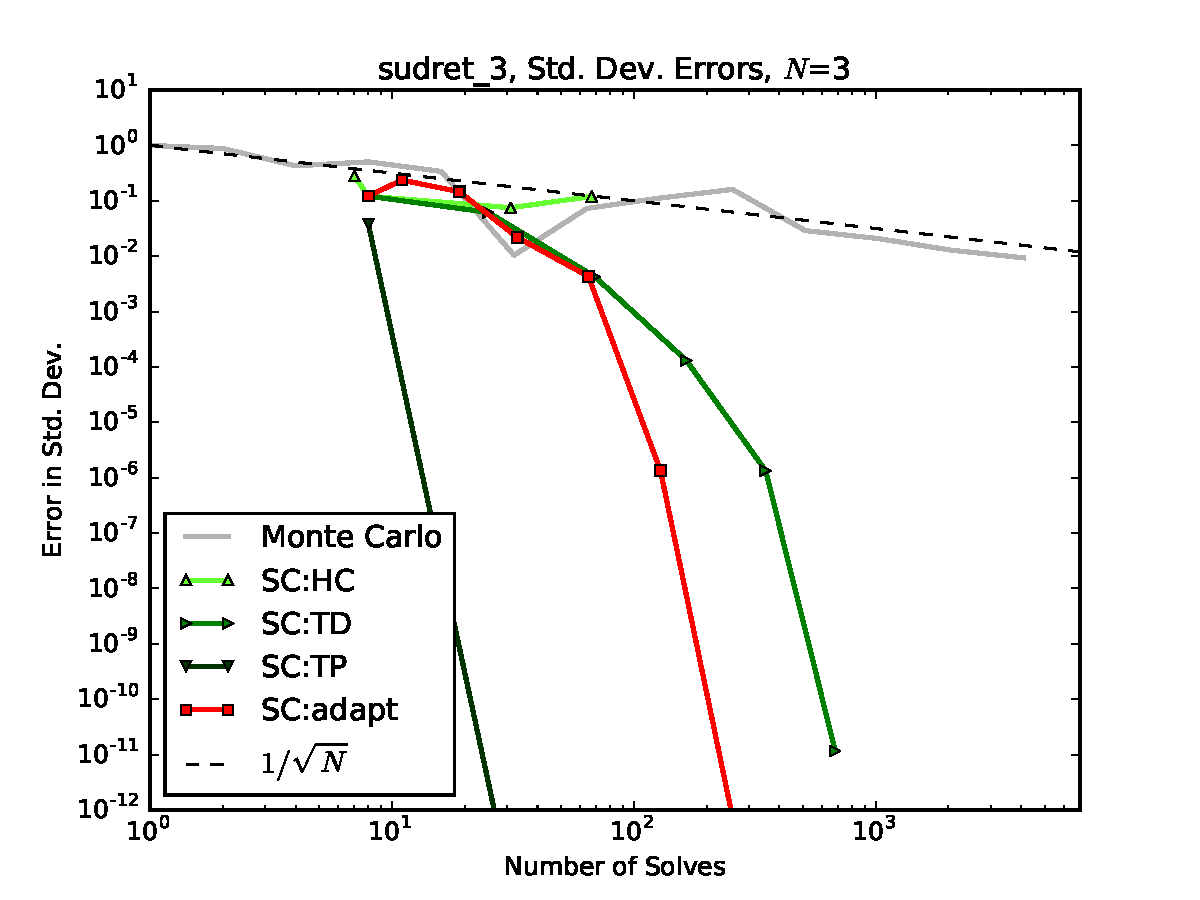
\includegraphics[width=0.8\linewidth]{anlmodels/sudret_3_variance_errs_nohdmr}
        \end{figure}
   \end{column}
 \end{columns}
\end{frame}
\begin{frame}{SCgPC Results}{Sudret Polynomials, $N=5$}\vspace{-20pt}
 \begin{columns}
   \begin{column}{0.5\textwidth}
        \begin{figure}[h!]
          \centering
          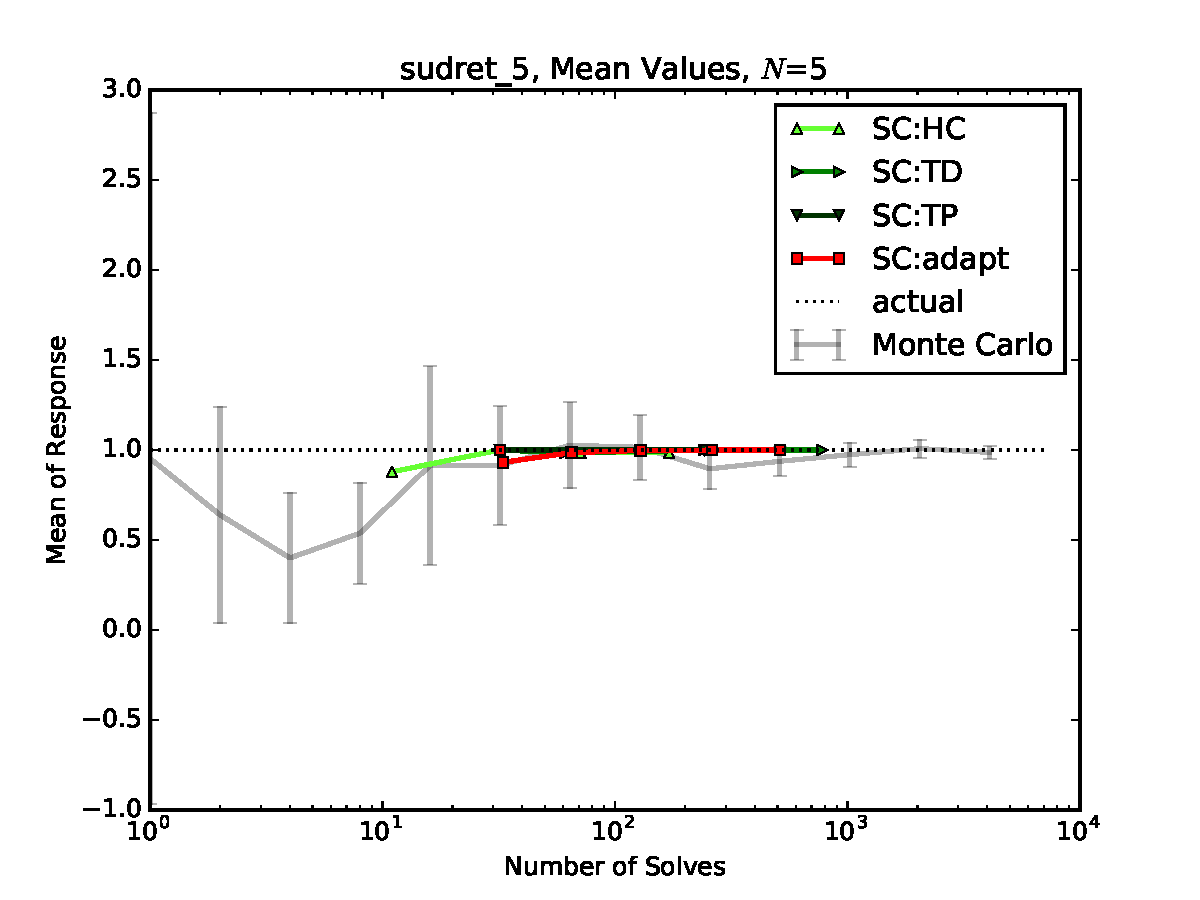
\includegraphics[width=0.8\linewidth]{anlmodels/sudret_5_mean_vals_nohdmr}
        \end{figure}
        \vspace{-20pt}
        \begin{figure}[h!]
          \centering
          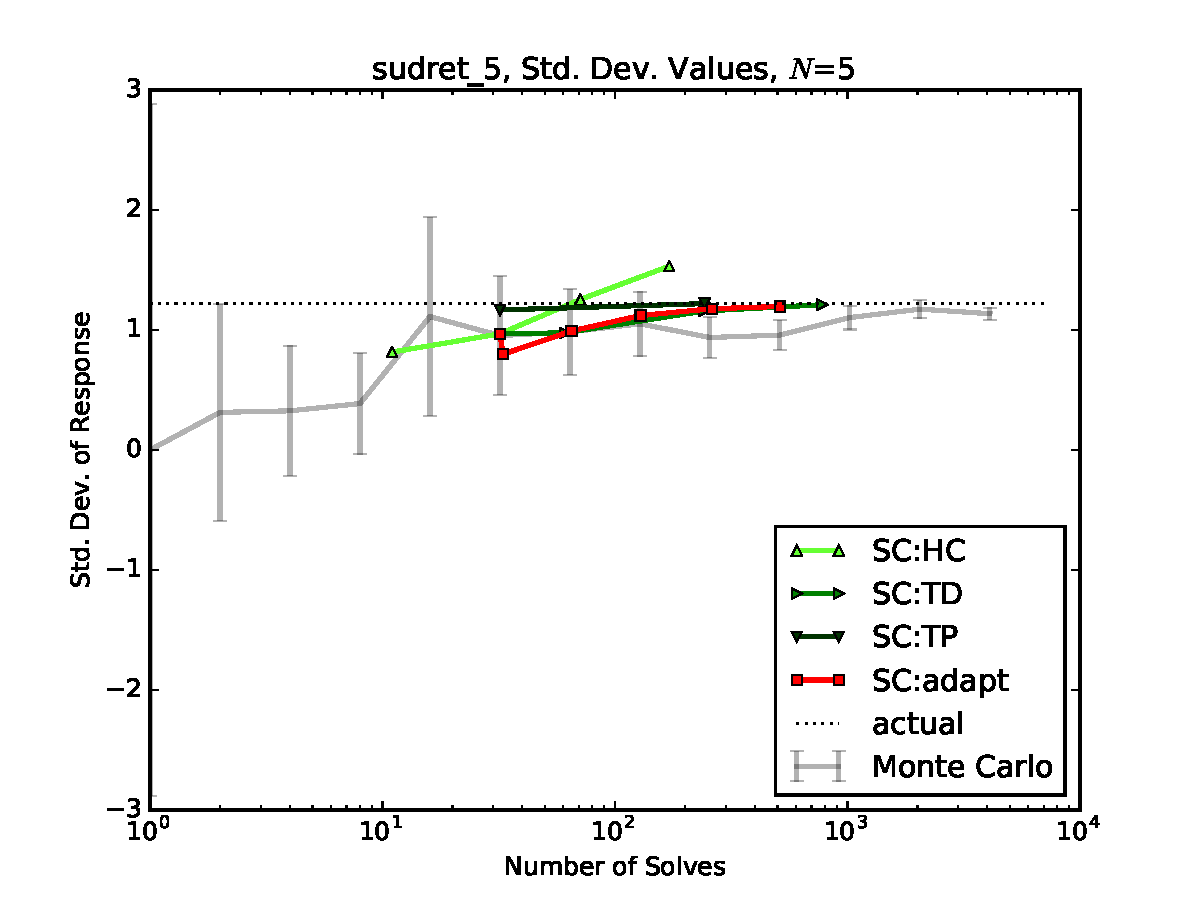
\includegraphics[width=0.8\linewidth]{anlmodels/sudret_5_var_vals_nohdmr}
        \end{figure}
   \end{column}
   \begin{column}{0.5\textwidth}
        \begin{figure}[h!]
          \centering
          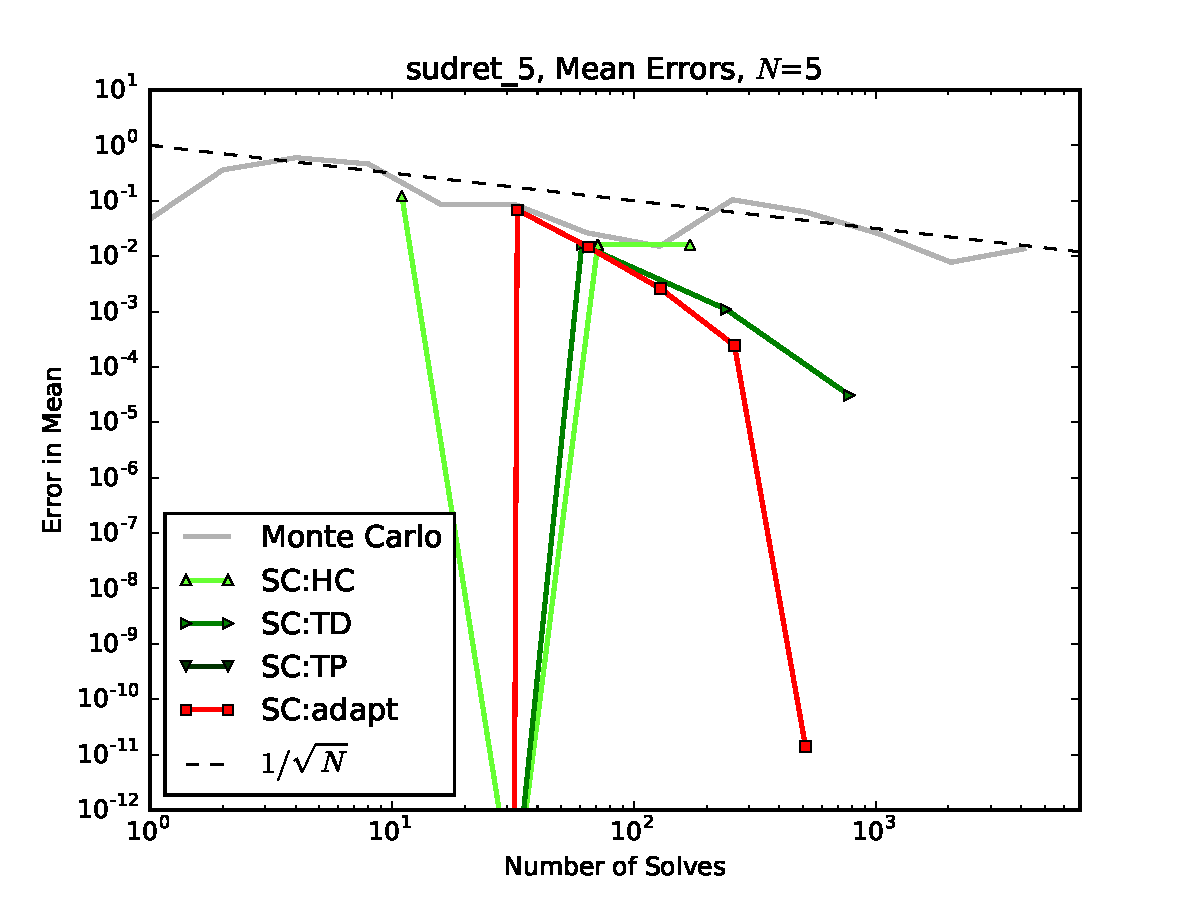
\includegraphics[width=0.8\linewidth]{anlmodels/sudret_5_mean_errs_nohdmr}
        \end{figure}
        \vspace{-20pt}
        \begin{figure}[h!]
          \centering
          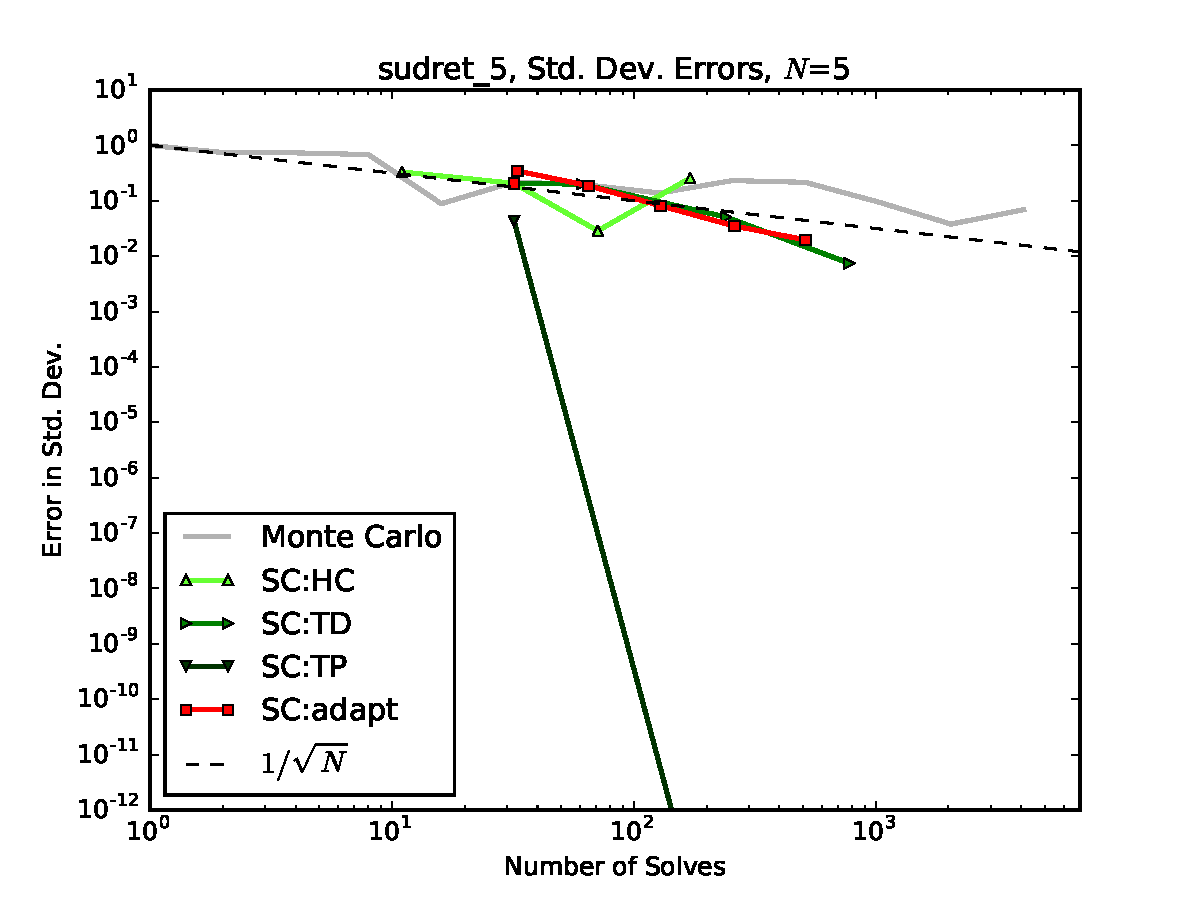
\includegraphics[width=0.8\linewidth]{anlmodels/sudret_5_variance_errs_nohdmr}
        \end{figure}
   \end{column}
 \end{columns}
\end{frame}


\subsubsection{Attenuation}
\begin{frame}{SCgPC Results}{Attenuation}\vspace{-20pt}
  \begin{columns}
    \begin{column}{0.6\textwidth}
      \begin{block}{Attenuation}
        \[u(Y) = \prod_{n=1}^N \exp(-y_n/N)\]
      \end{block}
    \end{column}
    \begin{column}{0.4\textwidth}
        \begin{figure}[h!]
          \centering
          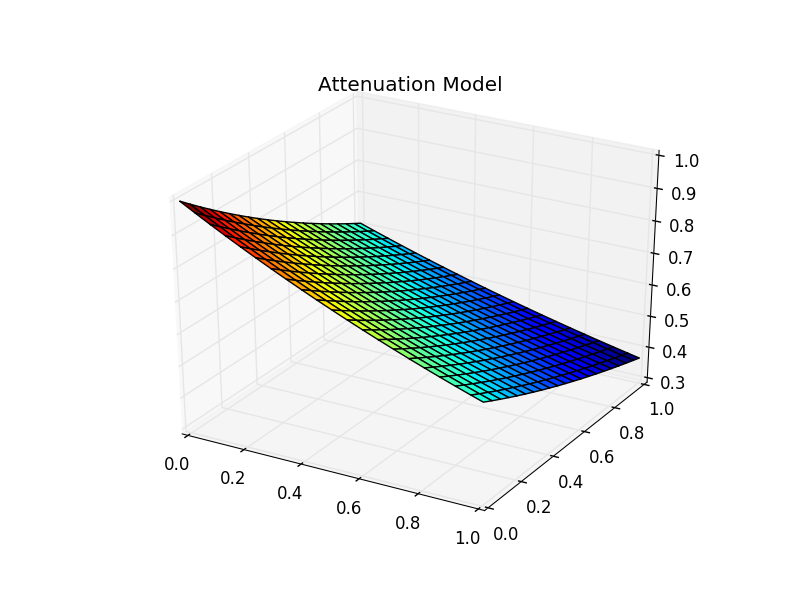
\includegraphics[width=\linewidth]{anlmodels/attenuate}
        \end{figure}
    \end{column}
  \end{columns}
  \begin{itemize}
    \item Tensor of decreasing-importance polynomials
    \item Combination terms over single-variable
  \end{itemize}
\end{frame}
\begin{frame}{SCgPC Results}{Attenuation, Taylor Expansion}%\vspace{-20pt}
  \begin{equation*}
    e^{-ay} = 1 - ay + \frac{(ay)^2}{2} - \frac{(ay)^3}{6} + \frac{(ay)^4}{24} - \frac{(ay)^5}{120} +
          \mathcal{O}(y^6)
  \end{equation*}
\begin{table}
  \centering
  \begin{tabular}{|c c|c c c c c|}
    \cline{3-7}\multicolumn{2}{c|}{ } & \multicolumn{5}{c|}{Polynomial Order ($y_1$)} \\
               \multicolumn{2}{c|}{ } & 0 & 1 & 2 & 3 & 4 \\
    \hline & 0 & 1        & $a$      & $a^2/2$  & $a^3/6$   & \cellcolor{Gray6}$a^4/24$  \\
Polynomial & 1 & $a$      & $a^2   $ & $a^3/2 $ & \cellcolor{Gray6}$a^4/6  $ & $a^5/24 $ \\
Order      & 2 & $a^2/2$  & $a^3/2 $ & \cellcolor{Gray6}$a^4/4 $ & $a^5/12 $ & $a^6/48 $ \\
($y_2$)    & 3 & $a^3/ 6$ & \cellcolor{Gray6}$a^4/ 6$ & $a^5/12$ & $a^6/ 36$ & $a^7/144$ \\
           & 4 & \cellcolor{Gray6}$a^4/24$ & $a^5/24$ & $a^6/48$ & $a^7/144$ & $a^8/576$ \\
    \hline
  \end{tabular}
\end{table}
\end{frame}
\begin{frame}{SCgPC Results}{Attenuation, $N=2$}\vspace{-20pt}
 \begin{columns}
   \begin{column}{0.5\textwidth}
        \begin{figure}[h!]
          \centering
          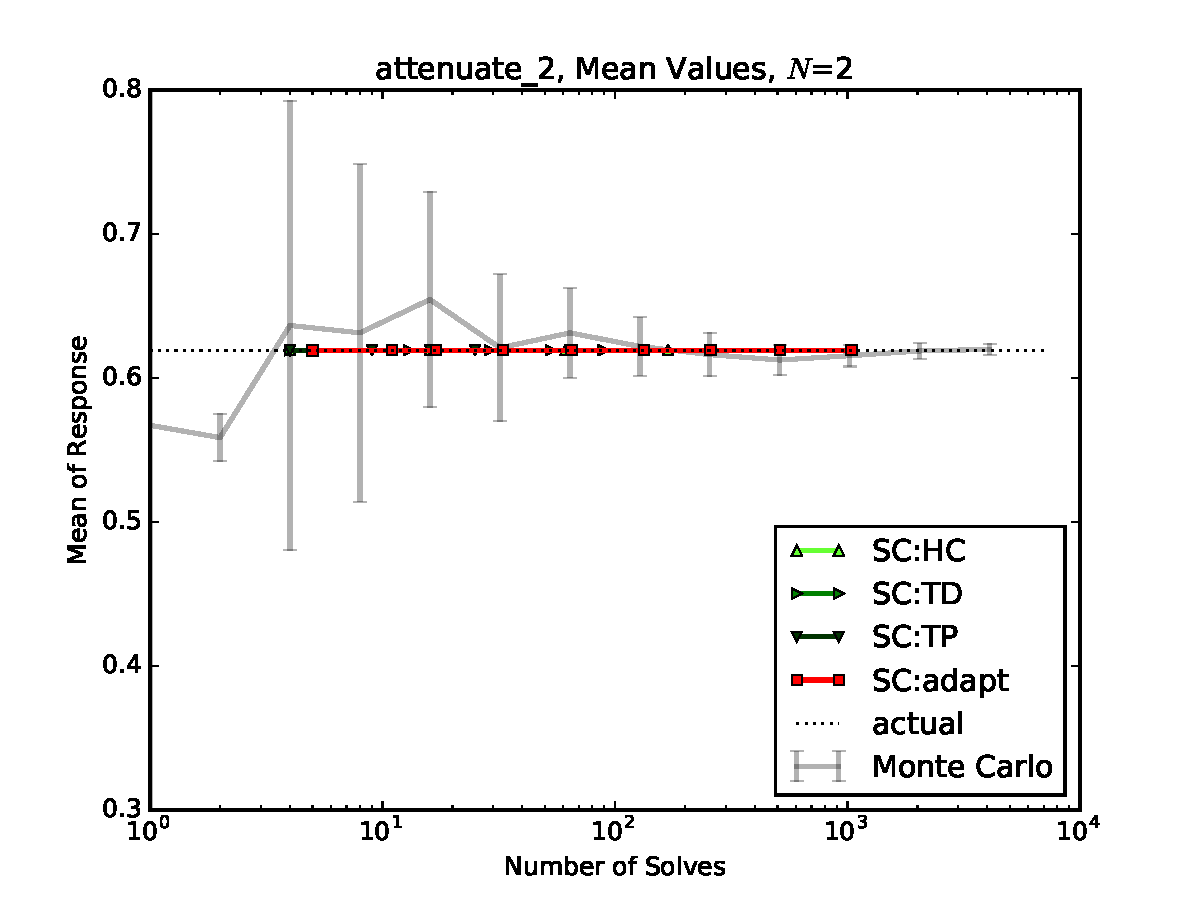
\includegraphics[width=0.8\linewidth]{anlmodels/attenuate_2_mean_vals_nohdmr}
        \end{figure}
        \vspace{-20pt}
        \begin{figure}[h!]
          \centering
          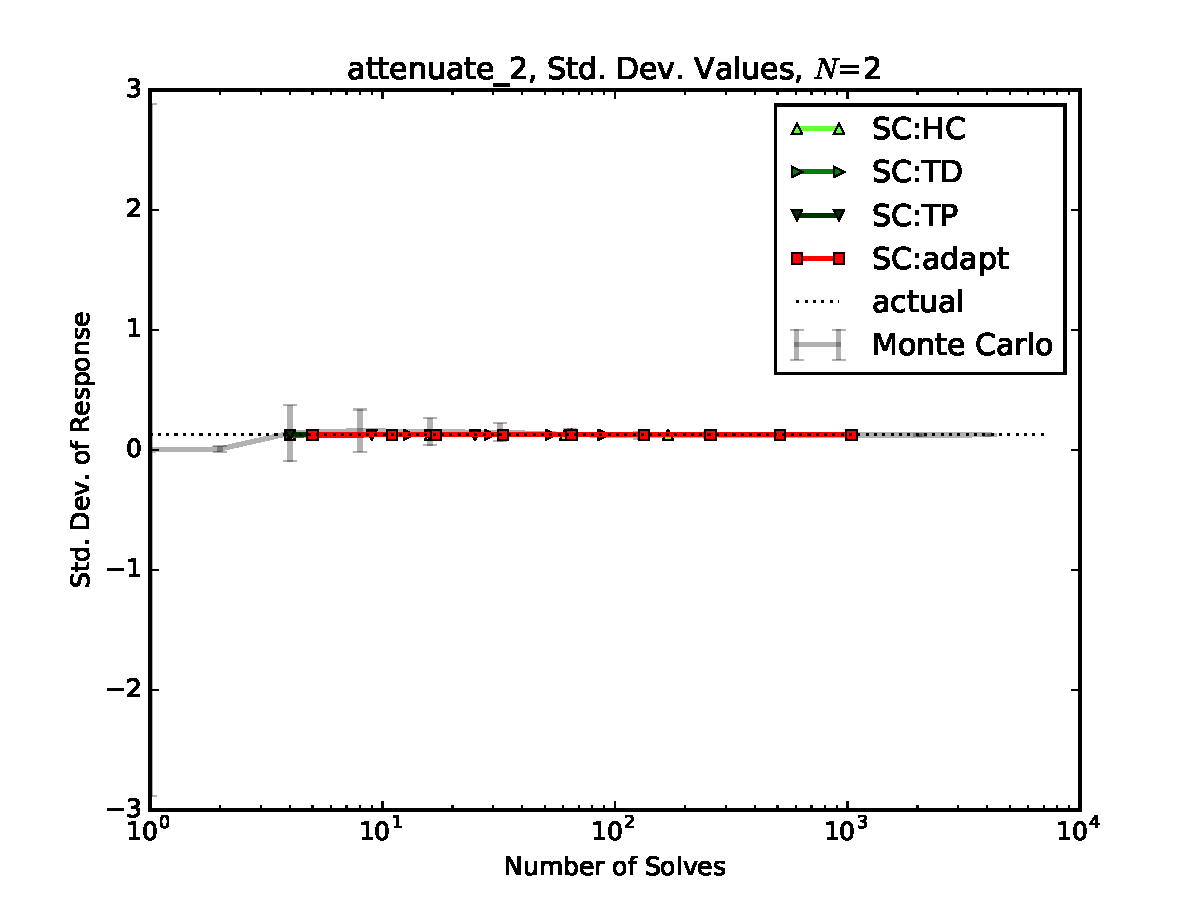
\includegraphics[width=0.8\linewidth]{anlmodels/attenuate_2_var_vals_nohdmr}
        \end{figure}
   \end{column}
   \begin{column}{0.5\textwidth}
        \begin{figure}[h!]
          \centering
          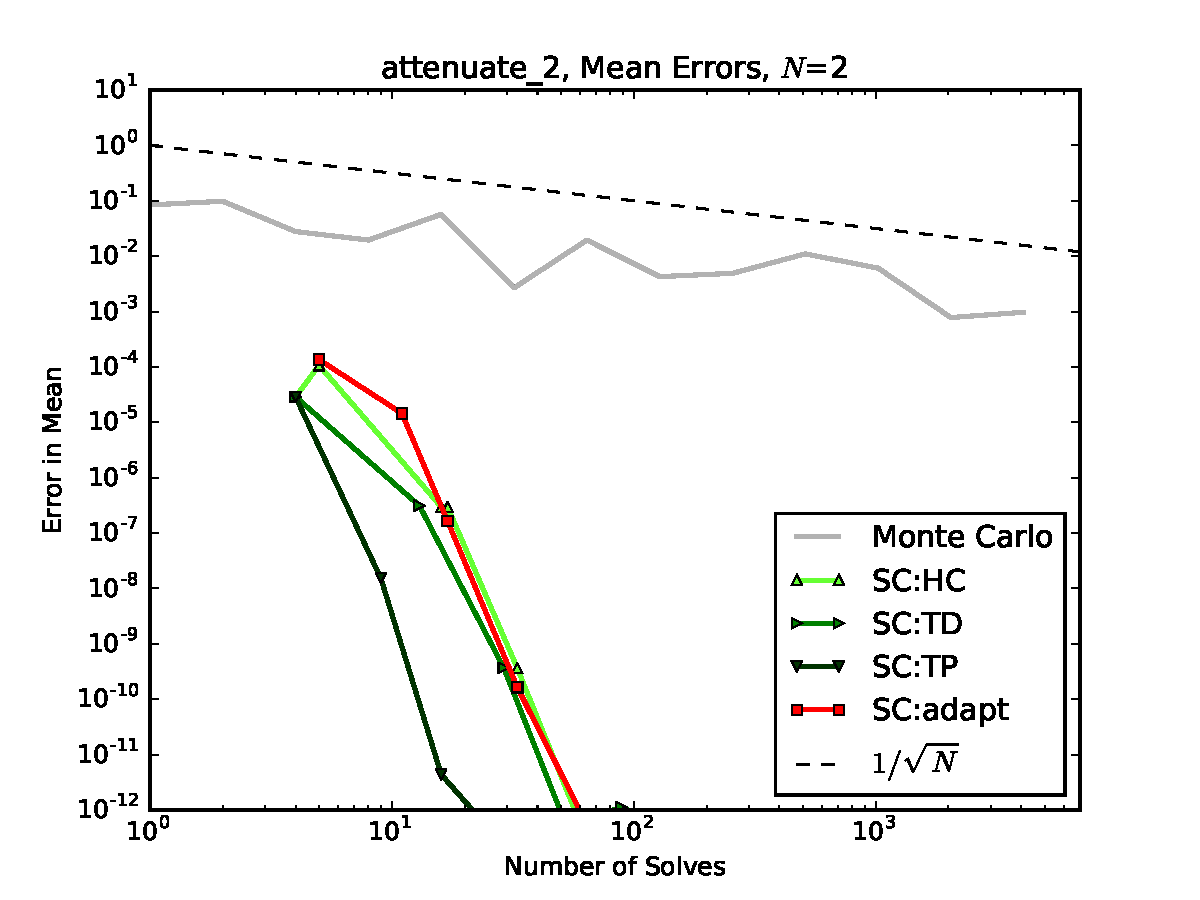
\includegraphics[width=0.8\linewidth]{anlmodels/attenuate_2_mean_errs_nohdmr}
        \end{figure}
        \vspace{-20pt}
        \begin{figure}[h!]
          \centering
          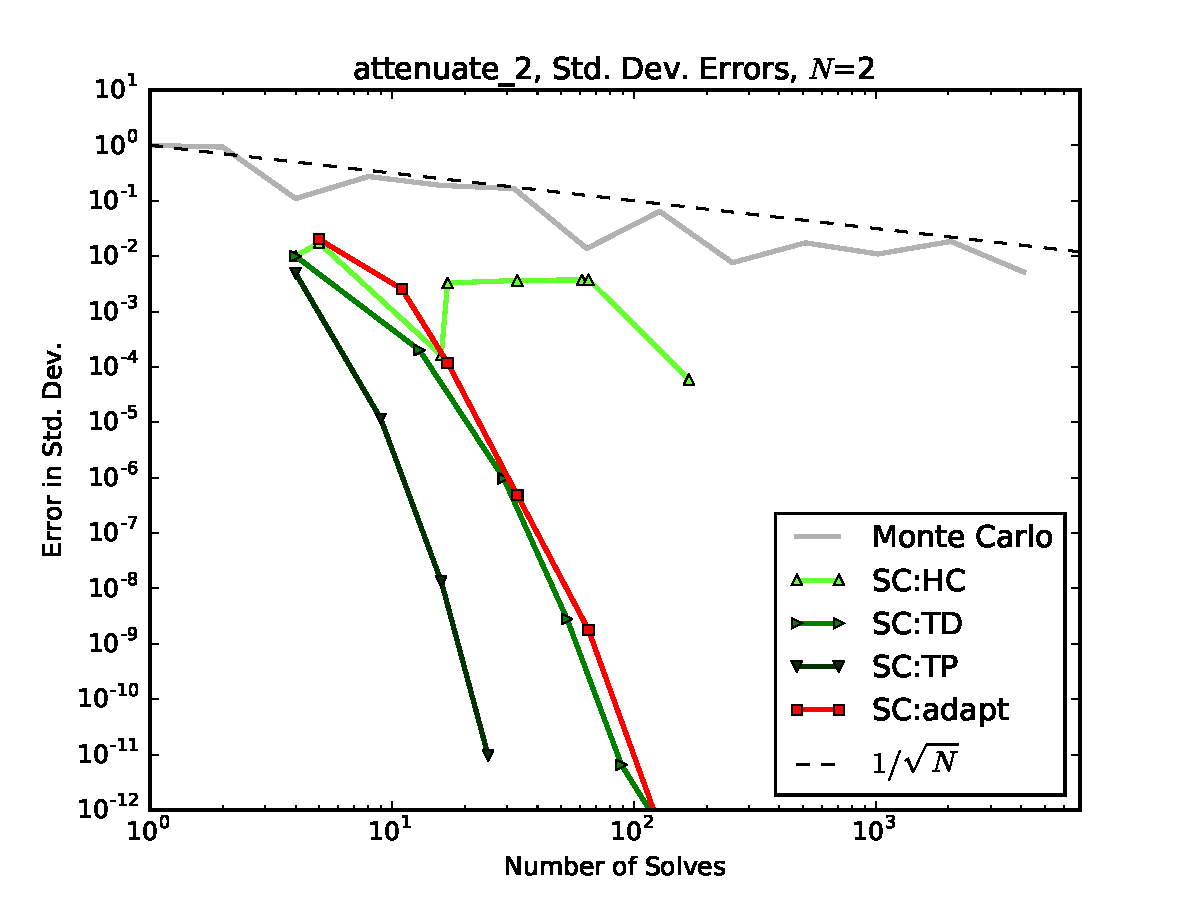
\includegraphics[width=0.8\linewidth]{anlmodels/attenuate_2_variance_errs_nohdmr}
        \end{figure}
   \end{column}
 \end{columns}
\end{frame}
\begin{frame}{SCgPC Results}{Attenuation, $N=4$}\vspace{-20pt}
 \begin{columns}
   \begin{column}{0.5\textwidth}
        \begin{figure}[h!]
          \centering
          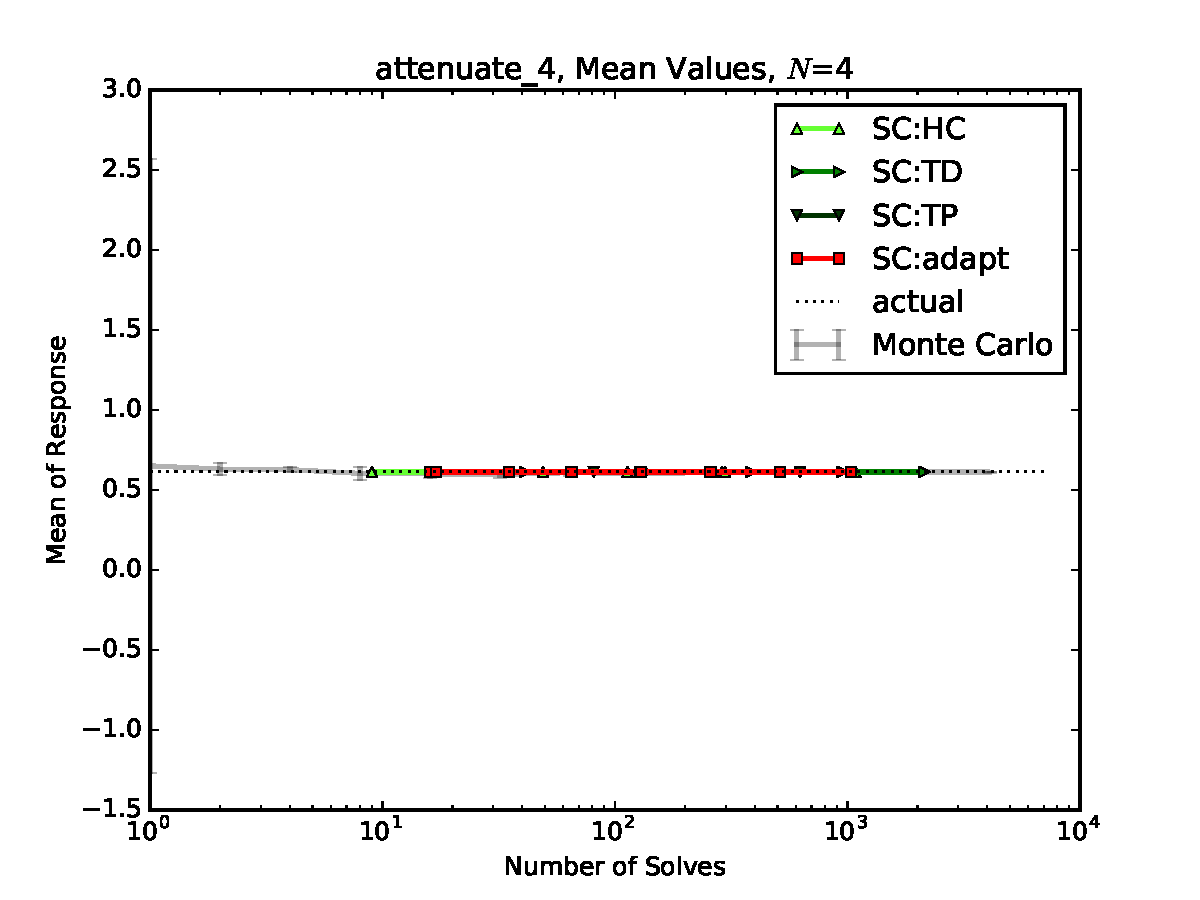
\includegraphics[width=0.8\linewidth]{anlmodels/attenuate_4_mean_vals_nohdmr}
        \end{figure}
        \vspace{-20pt}
        \begin{figure}[h!]
          \centering
          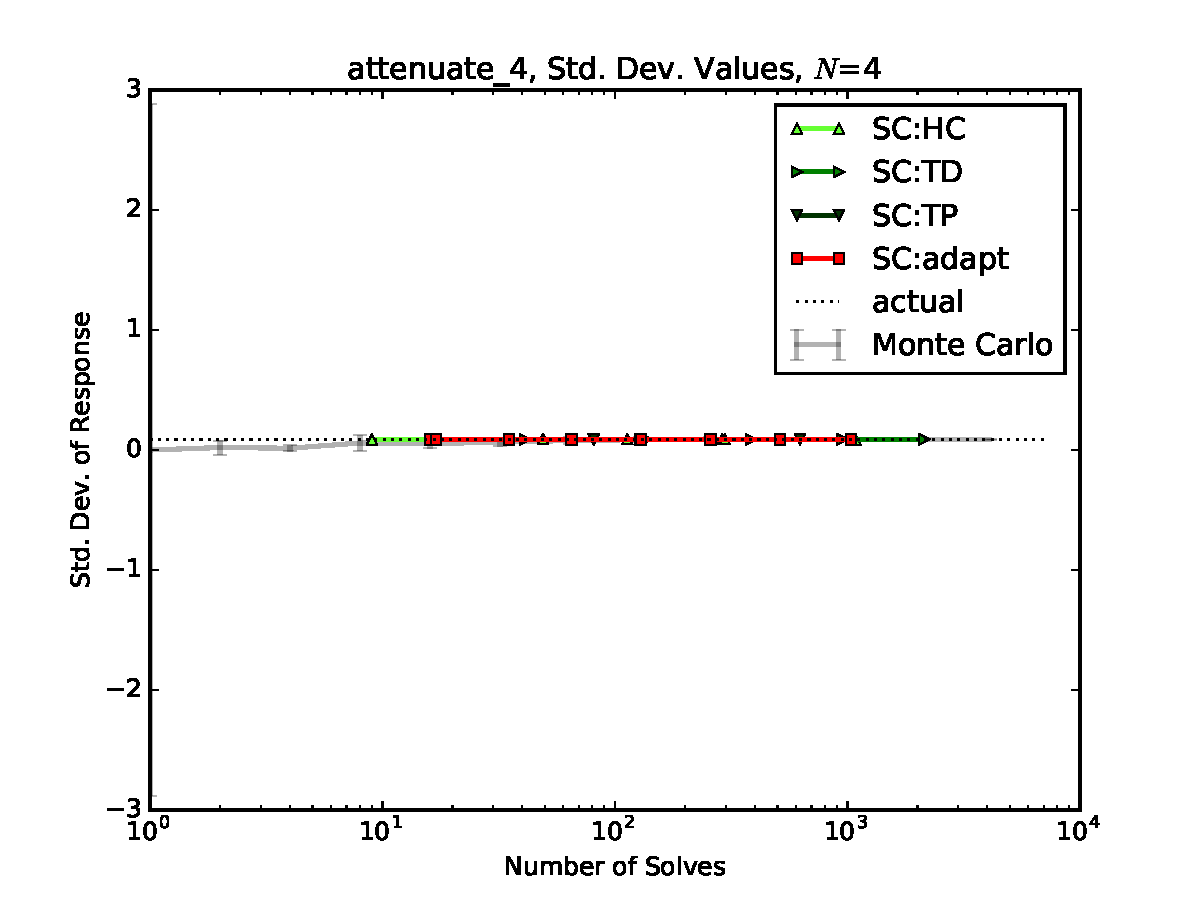
\includegraphics[width=0.8\linewidth]{anlmodels/attenuate_4_var_vals_nohdmr}
        \end{figure}
   \end{column}
   \begin{column}{0.5\textwidth}
        \begin{figure}[h!]
          \centering
          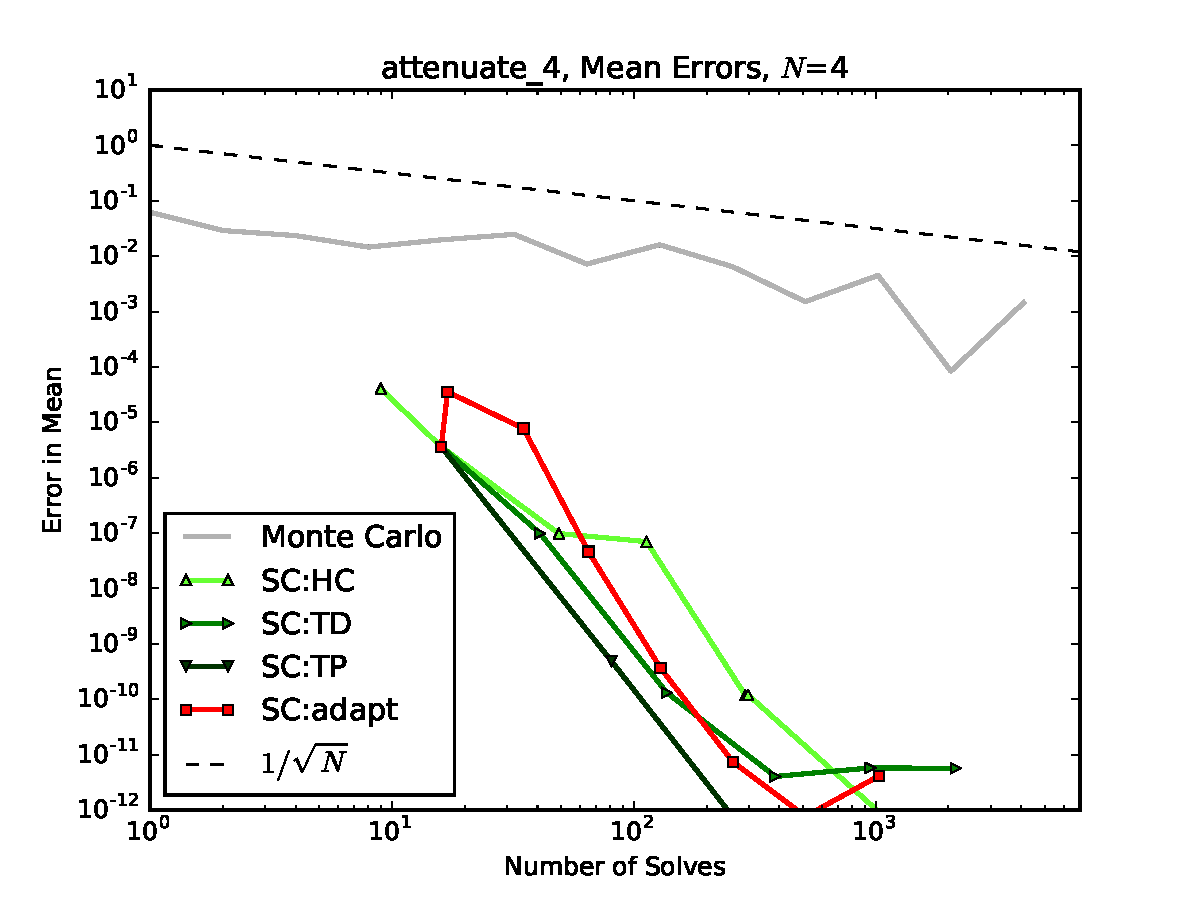
\includegraphics[width=0.8\linewidth]{anlmodels/attenuate_4_mean_errs_nohdmr}
        \end{figure}
        \vspace{-20pt}
        \begin{figure}[h!]
          \centering
          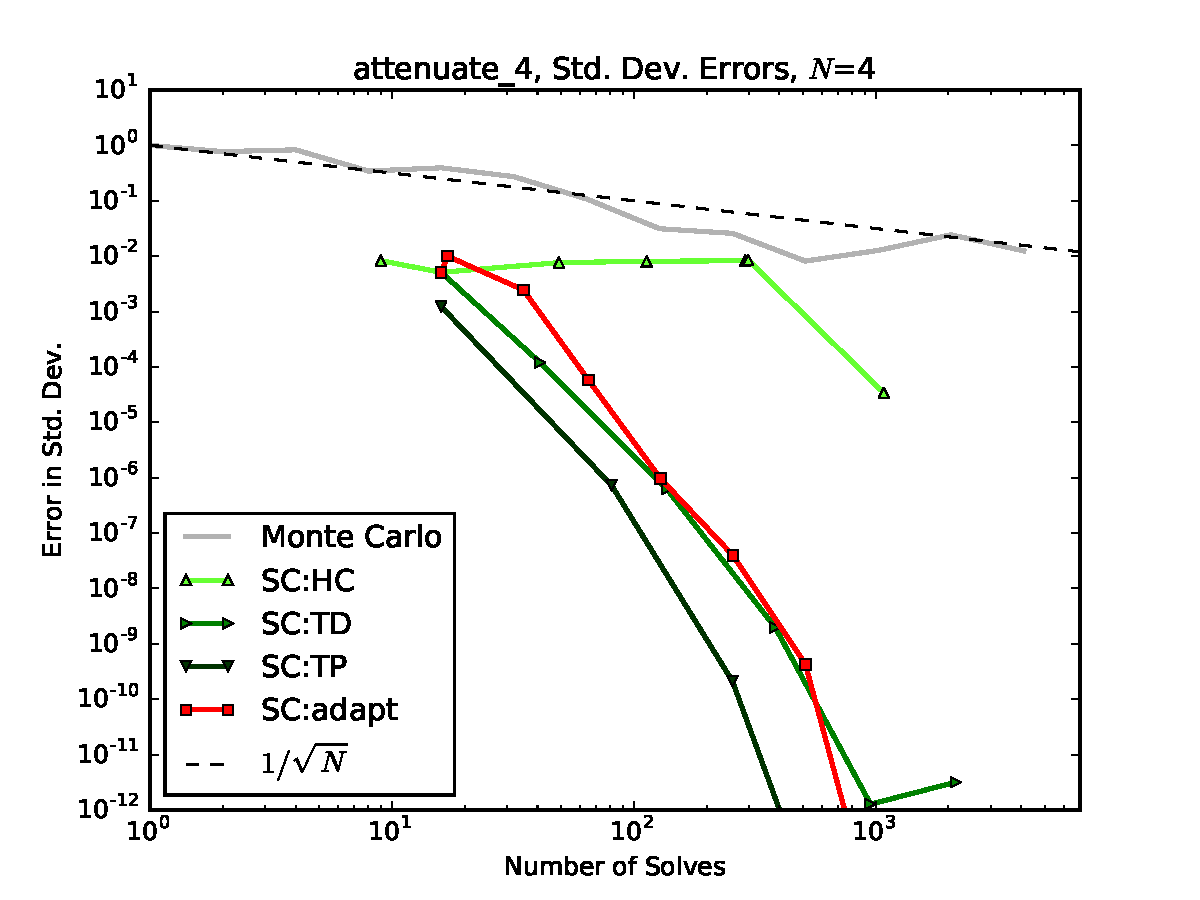
\includegraphics[width=0.8\linewidth]{anlmodels/attenuate_4_variance_errs_nohdmr}
        \end{figure}
   \end{column}
 \end{columns}
\end{frame}
\begin{frame}{SCgPC Results}{Attenuation, $N=6$}\vspace{-20pt}
 \begin{columns}
   \begin{column}{0.5\textwidth}
        \begin{figure}[h!]
          \centering
          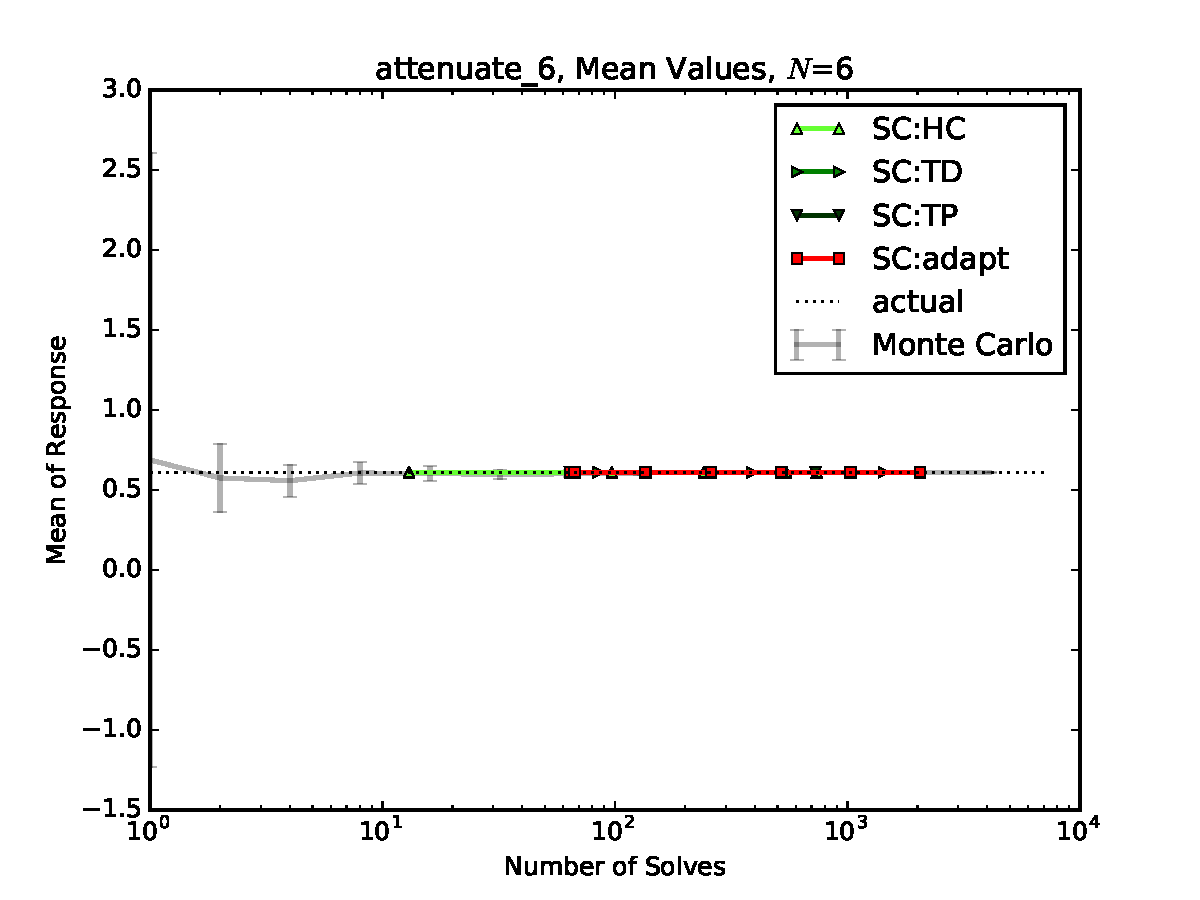
\includegraphics[width=0.8\linewidth]{anlmodels/attenuate_6_mean_vals_nohdmr}
        \end{figure}
        \vspace{-20pt}
        \begin{figure}[h!]
          \centering
          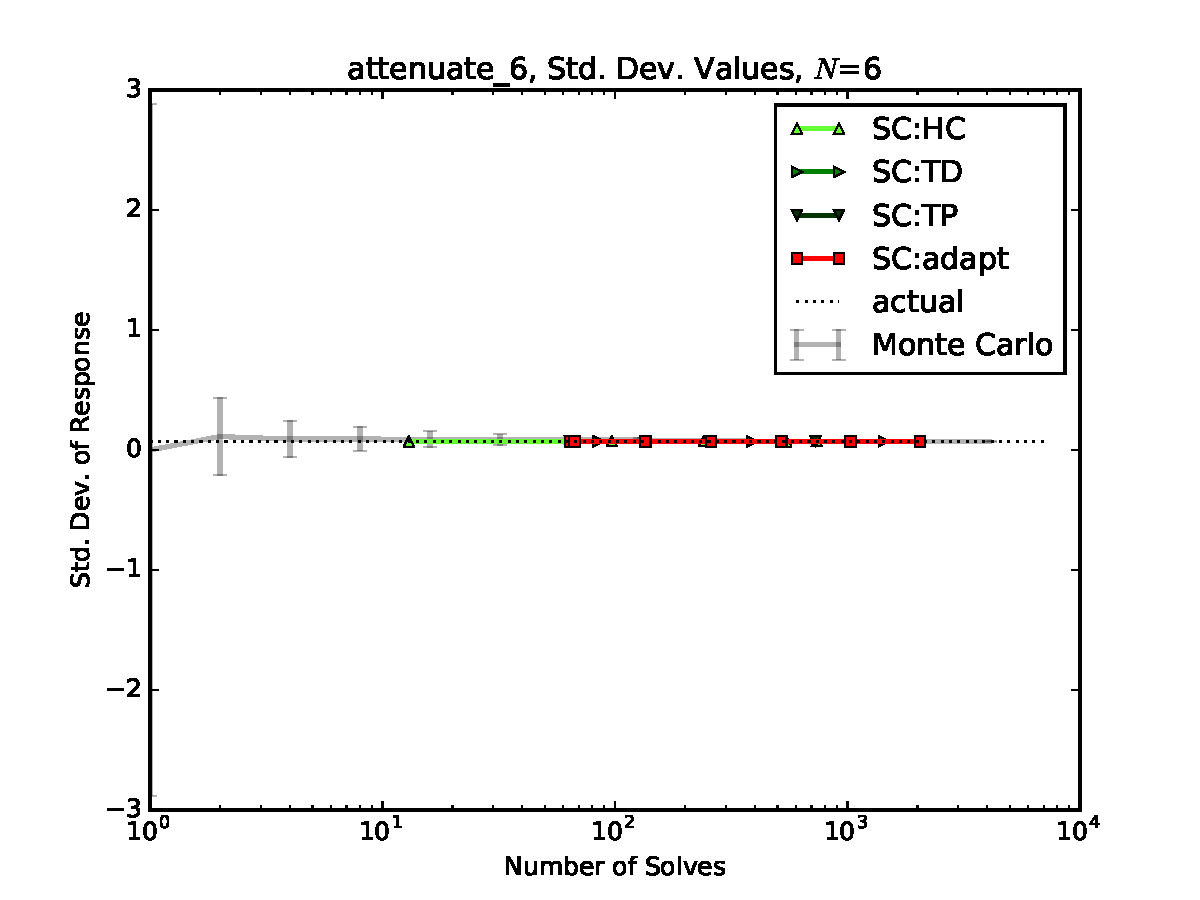
\includegraphics[width=0.8\linewidth]{anlmodels/attenuate_6_var_vals_nohdmr}
        \end{figure}
   \end{column}
   \begin{column}{0.5\textwidth}
        \begin{figure}[h!]
          \centering
          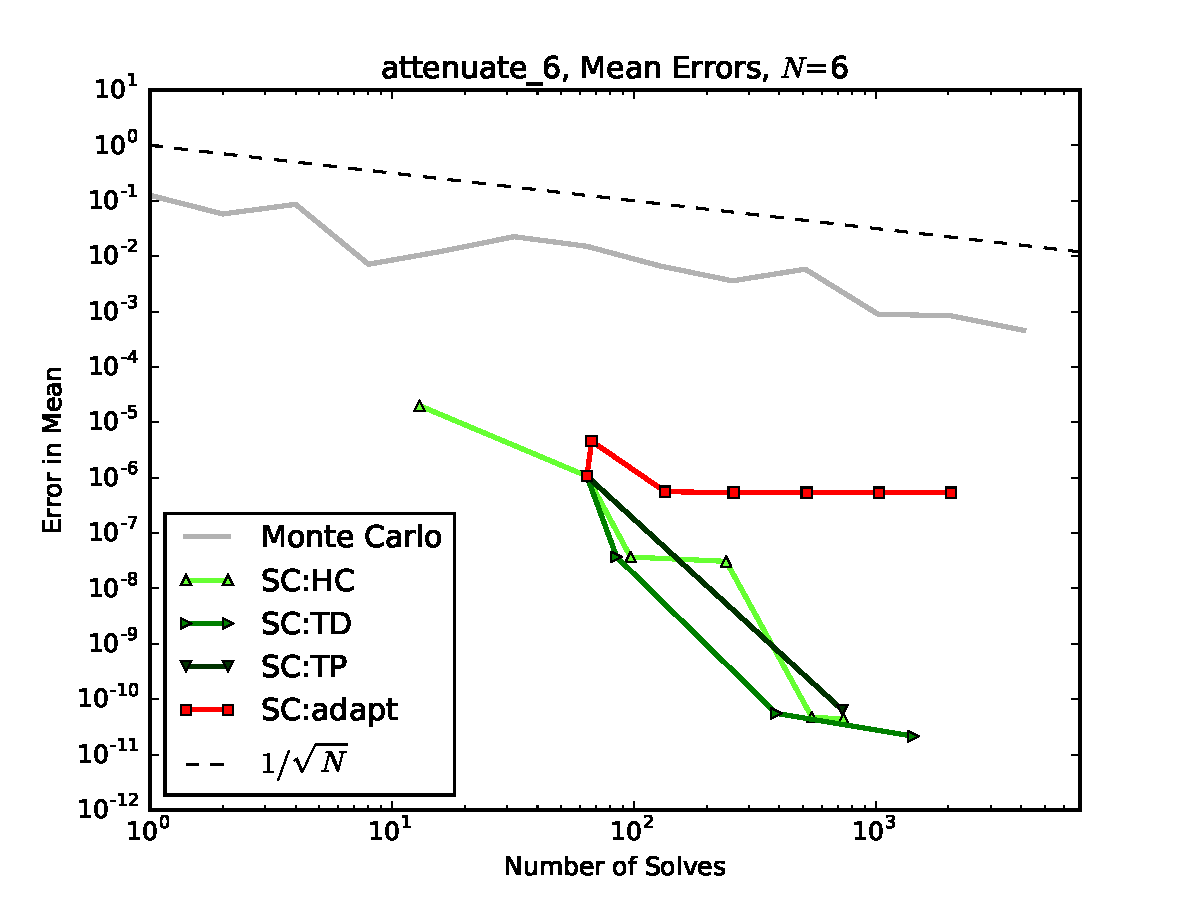
\includegraphics[width=0.8\linewidth]{anlmodels/attenuate_6_mean_errs_nohdmr}
        \end{figure}
        \vspace{-20pt}
        \begin{figure}[h!]
          \centering
          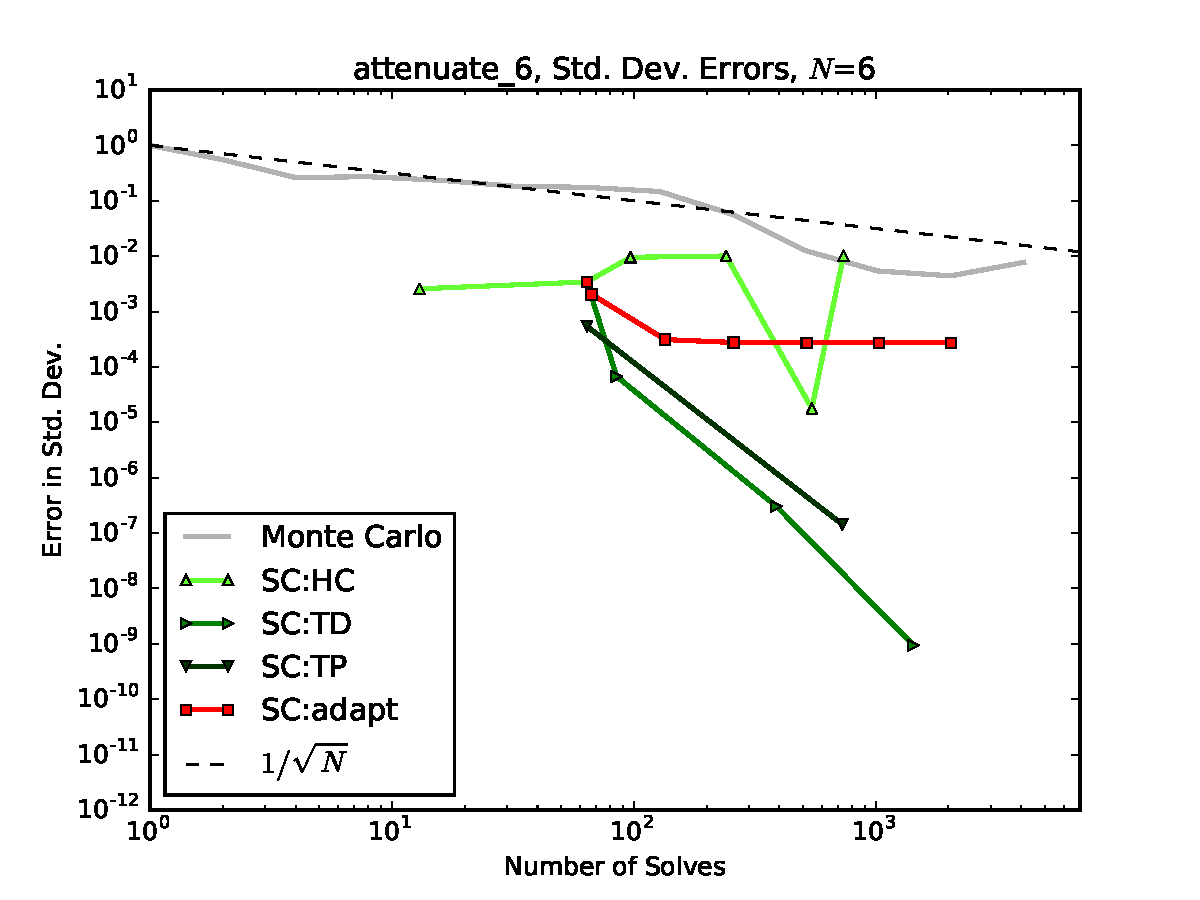
\includegraphics[width=0.8\linewidth]{anlmodels/attenuate_6_variance_errs_nohdmr}
        \end{figure}
   \end{column}
 \end{columns}
\end{frame}




\subsubsection{Gauss Peak}
\begin{frame}{SCgPC Results}{Gauss Peak}\vspace{-20pt}
  \begin{columns}
    \begin{column}{0.6\textwidth}
      \begin{block}{Gauss Peak}
        \[u(Y) = \prod_{n=1}^N \exp(-3^2(y_n-0.5)^2)\]
      \end{block}
    \end{column}
    \begin{column}{0.4\textwidth}
        \begin{figure}[h!]
          \centering
          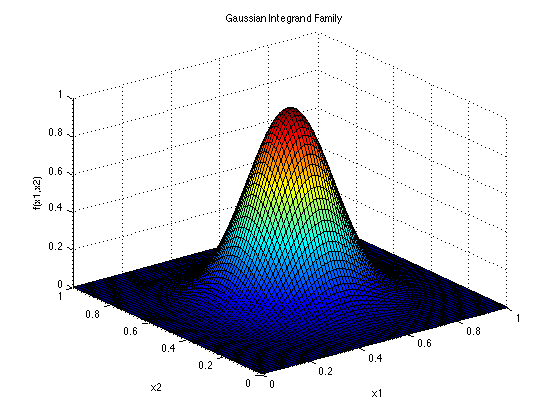
\includegraphics[width=\linewidth]{anlmodels/gaussian}
        \end{figure}
    \end{column}
  \end{columns}
  \begin{itemize}
    \item Tensor of polynomials
    \item Slow, inconsistent decay
  \end{itemize}
\end{frame}
\begin{frame}{SCgPC Results}{Gauss Peak, Taylor Expansion}\vspace{-20pt}
\begin{equation*}
  e^{-a^2y^2} = 1 - a^2y^2 + \frac{a^4}{2}y^4 - \frac{a^6}{6}y^6 + \frac{a^8}{24}y^8 + \mathcal{O}(y^{10})
\end{equation*}
\begin{table}
  \centering
  \begin{tabular}{|c c|c c c c c|}
    \cline{3-7}\multicolumn{2}{c|}{ } & \multicolumn{5}{c|}{Polynomial Order ($y_1$)} \\
\multicolumn{2}{c|}{ } & 0       & 1 & 2       & 3 & 4       \\
    \hline         & 0 & 1       & 0 & $a^2$   & 0 & $a^4/2$ \\
Polynomial         & 1 & 0       & 0 & 0       & 0 & 0       \\
Order              & 2 & $a^2$   & 0 & $a^4$   & 0 & $a^6/2$ \\
($y_2$)            & 3 & 0       & 0 & 0       & 0 & 0       \\
                   & 4 & $a^4/2$ & 0 & $a^6/2$ & 0 & $a^8/4$ \\
    \hline
  \end{tabular}
\end{table}
\end{frame}
\begin{frame}{SCgPC Results}{Gauss Peak, $N=3$}\vspace{-20pt}
 \begin{columns}
   \begin{column}{0.5\textwidth}
        \begin{figure}[h!]
          \centering
          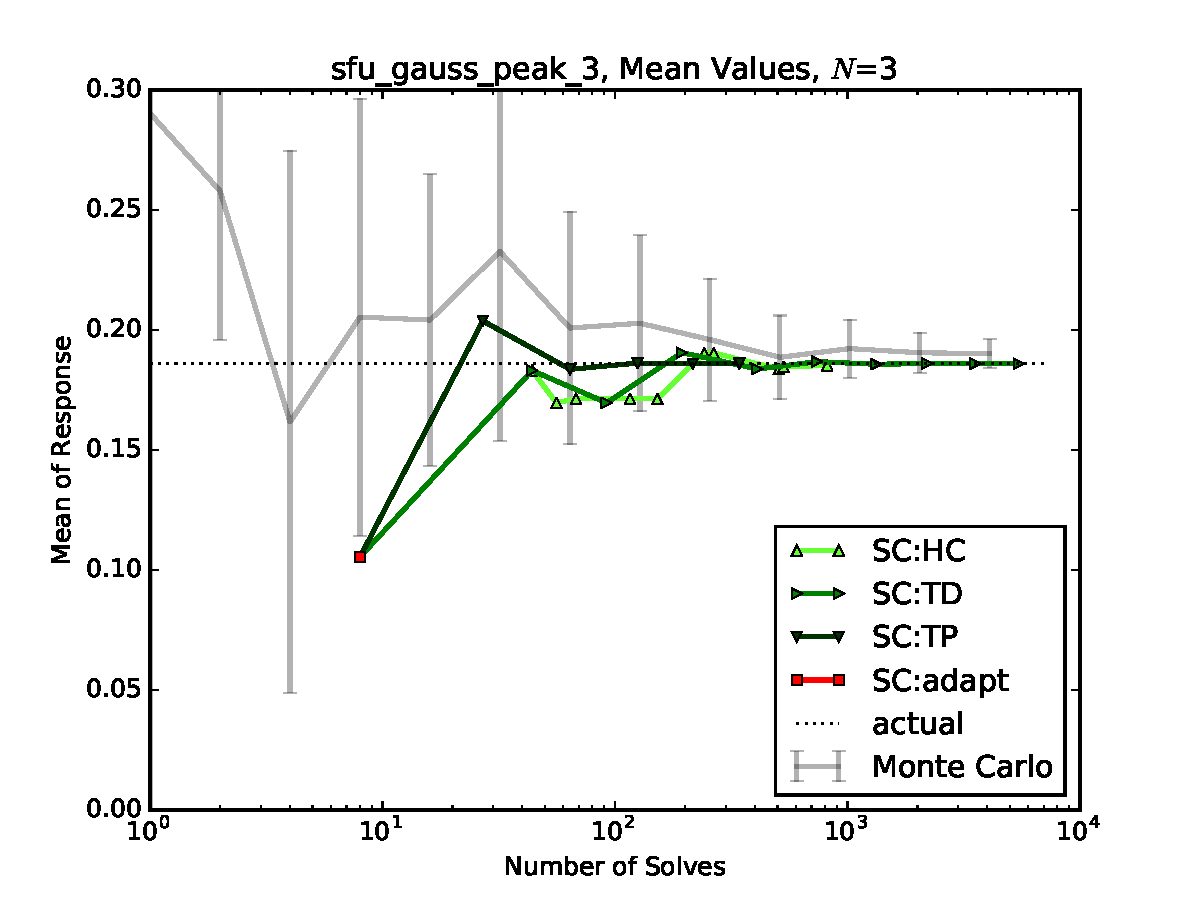
\includegraphics[width=0.8\linewidth]{anlmodels/sfu_gauss_peak_3_mean_vals_nohdmr}
        \end{figure}
        \vspace{-20pt}
        \begin{figure}[h!]
          \centering
          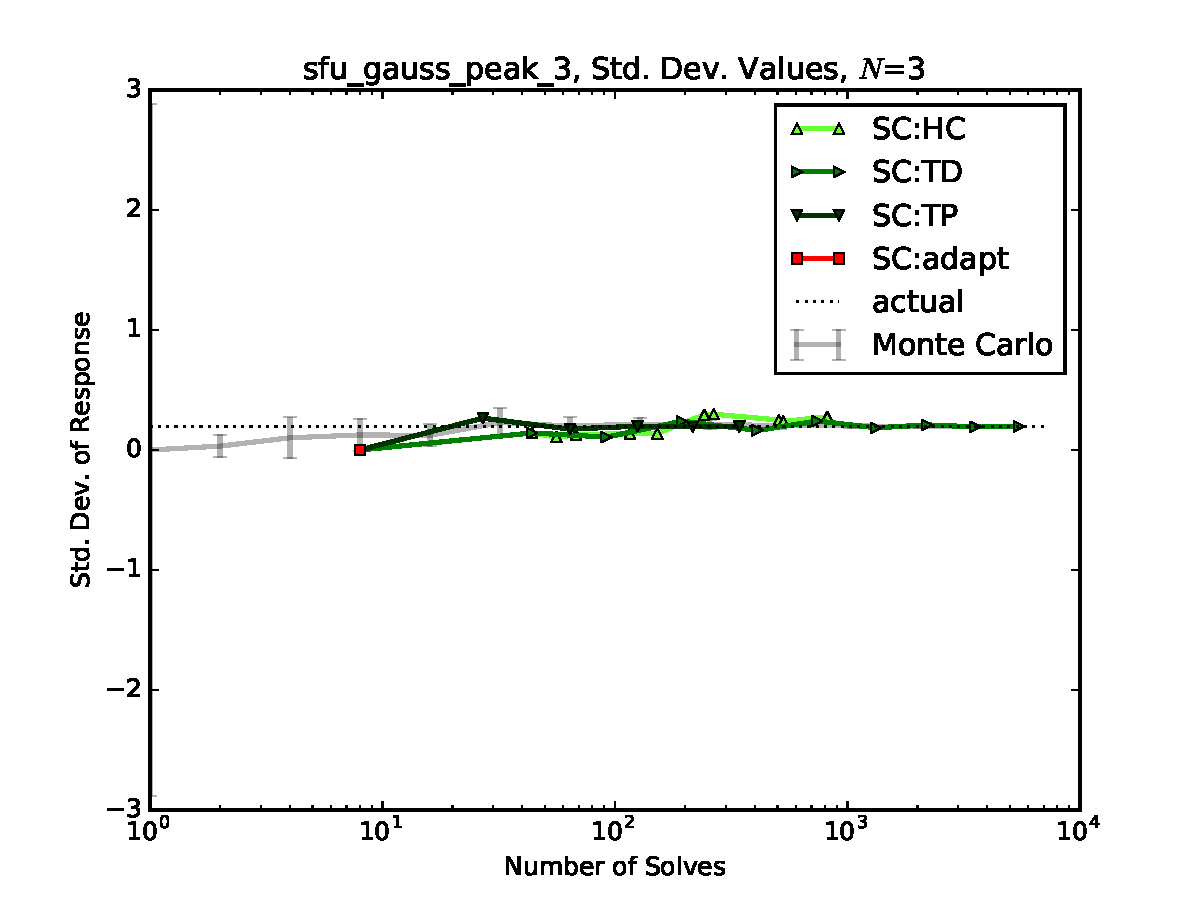
\includegraphics[width=0.8\linewidth]{anlmodels/sfu_gauss_peak_3_var_vals_nohdmr}
        \end{figure}
   \end{column}
   \begin{column}{0.5\textwidth}
        \begin{figure}[h!]
          \centering
          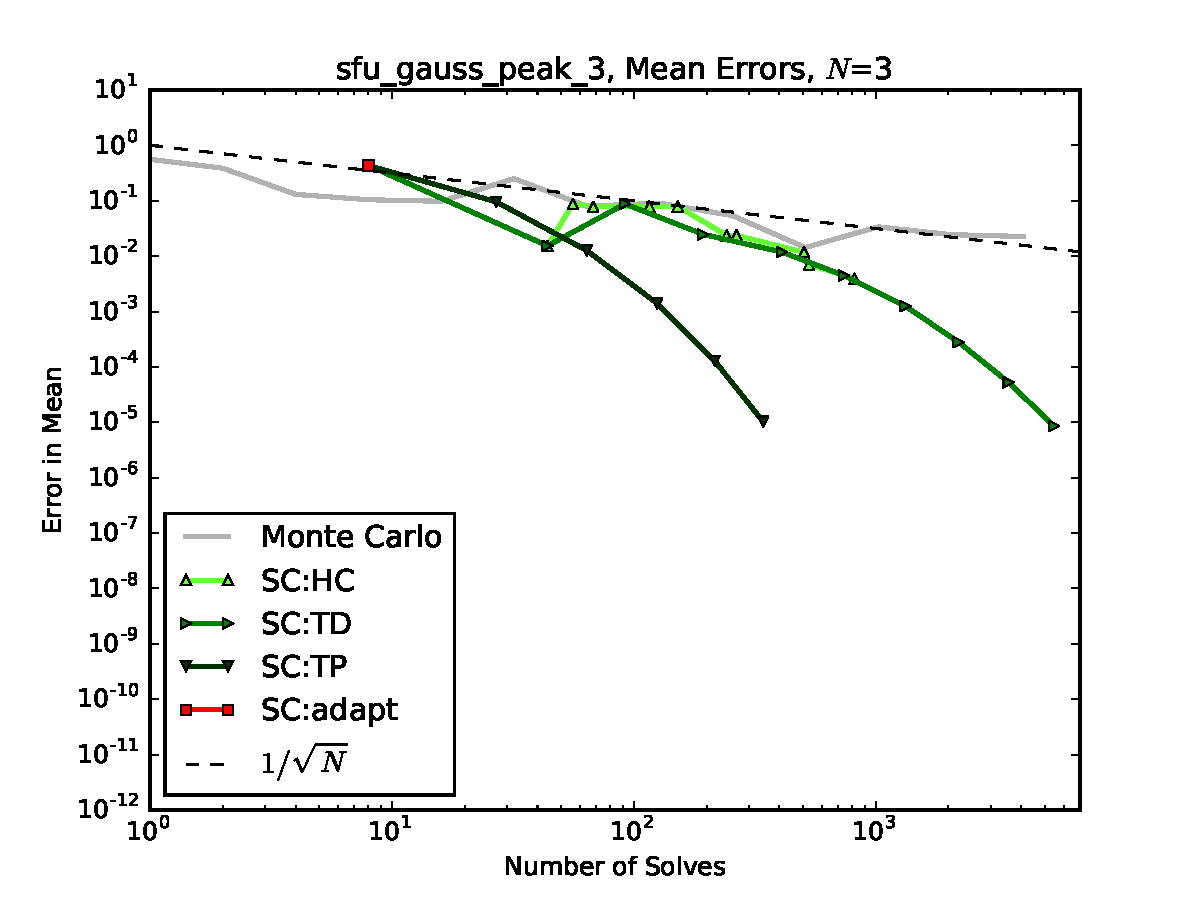
\includegraphics[width=0.8\linewidth]{anlmodels/sfu_gauss_peak_3_mean_errs_nohdmr}
        \end{figure}
        \vspace{-20pt}
        \begin{figure}[h!]
          \centering
          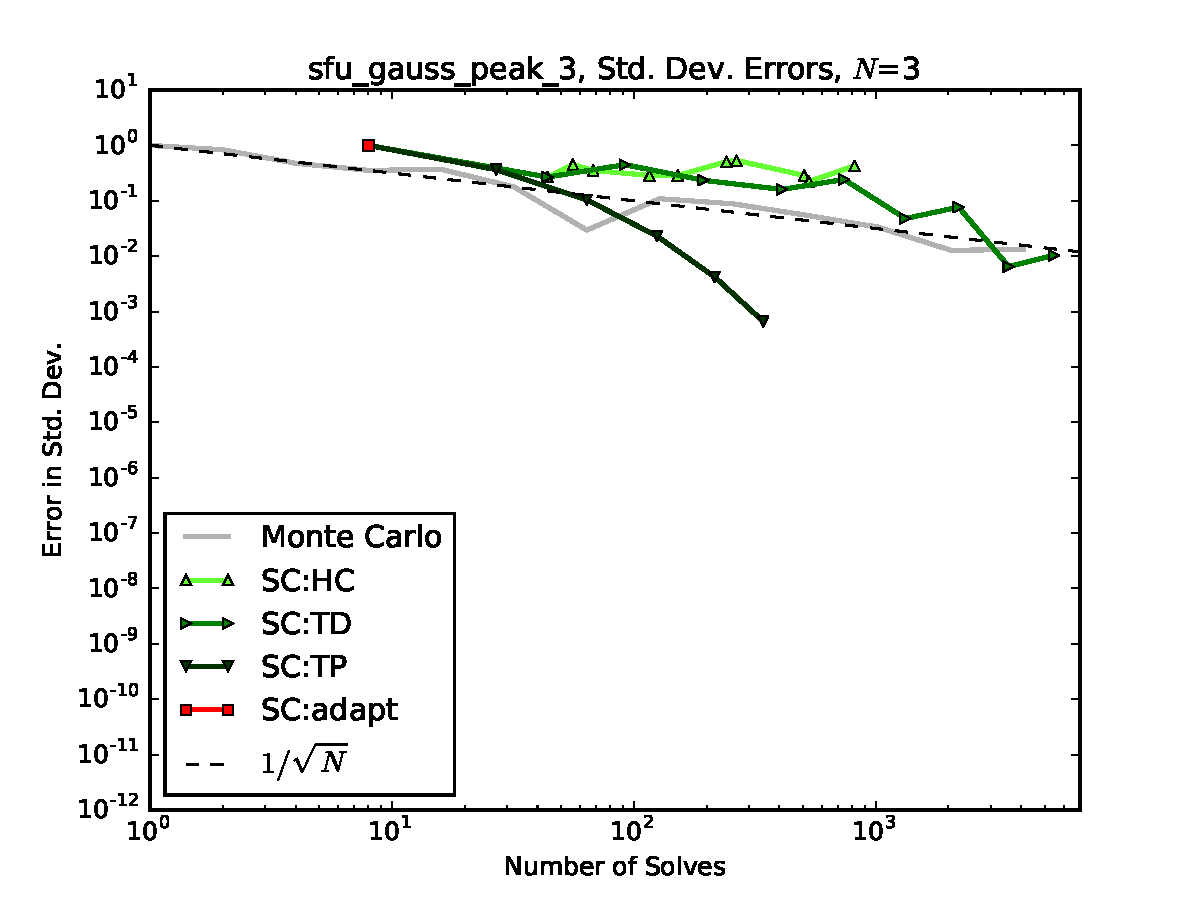
\includegraphics[width=0.8\linewidth]{anlmodels/sfu_gauss_peak_3_variance_errs_nohdmr}
        \end{figure}
   \end{column}
 \end{columns}
\end{frame}
\begin{frame}{SCgPC Results}{Gauss Peak, $N=5$}\vspace{-20pt}
 \begin{columns}
   \begin{column}{0.5\textwidth}
        \begin{figure}[h!]
          \centering
          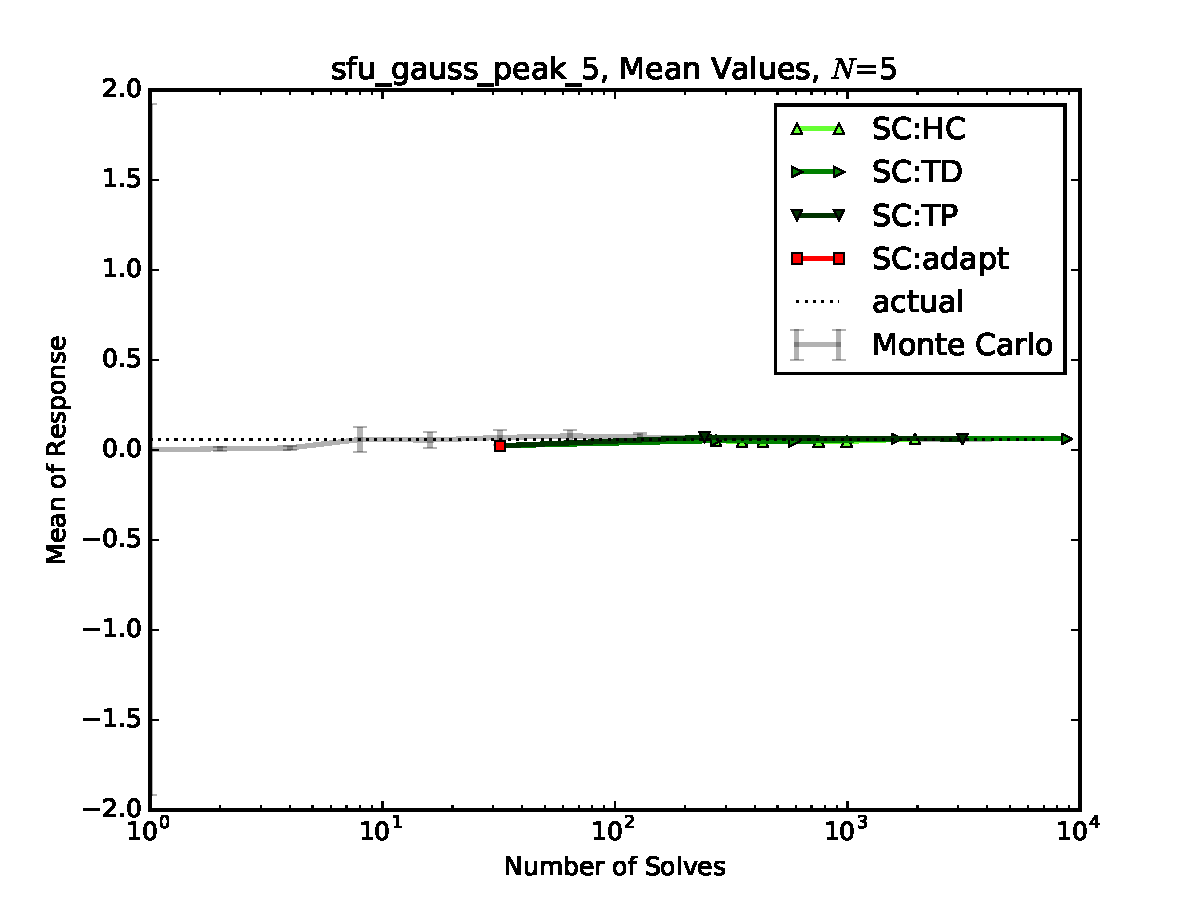
\includegraphics[width=0.8\linewidth]{anlmodels/sfu_gauss_peak_5_mean_vals_nohdmr}
        \end{figure}
        \vspace{-20pt}
        \begin{figure}[h!]
          \centering
          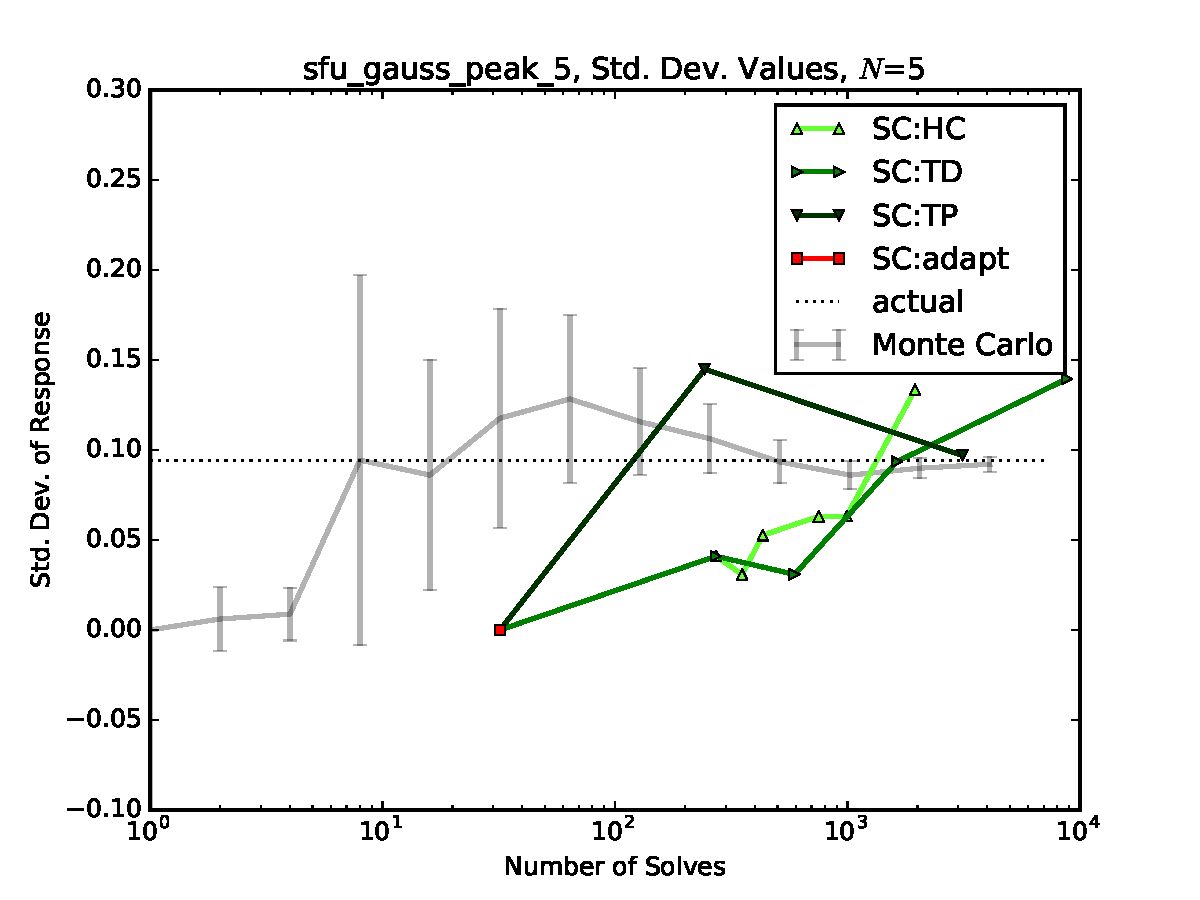
\includegraphics[width=0.8\linewidth]{anlmodels/sfu_gauss_peak_5_var_vals_nohdmr}
        \end{figure}
   \end{column}
   \begin{column}{0.5\textwidth}
        \begin{figure}[h!]
          \centering
          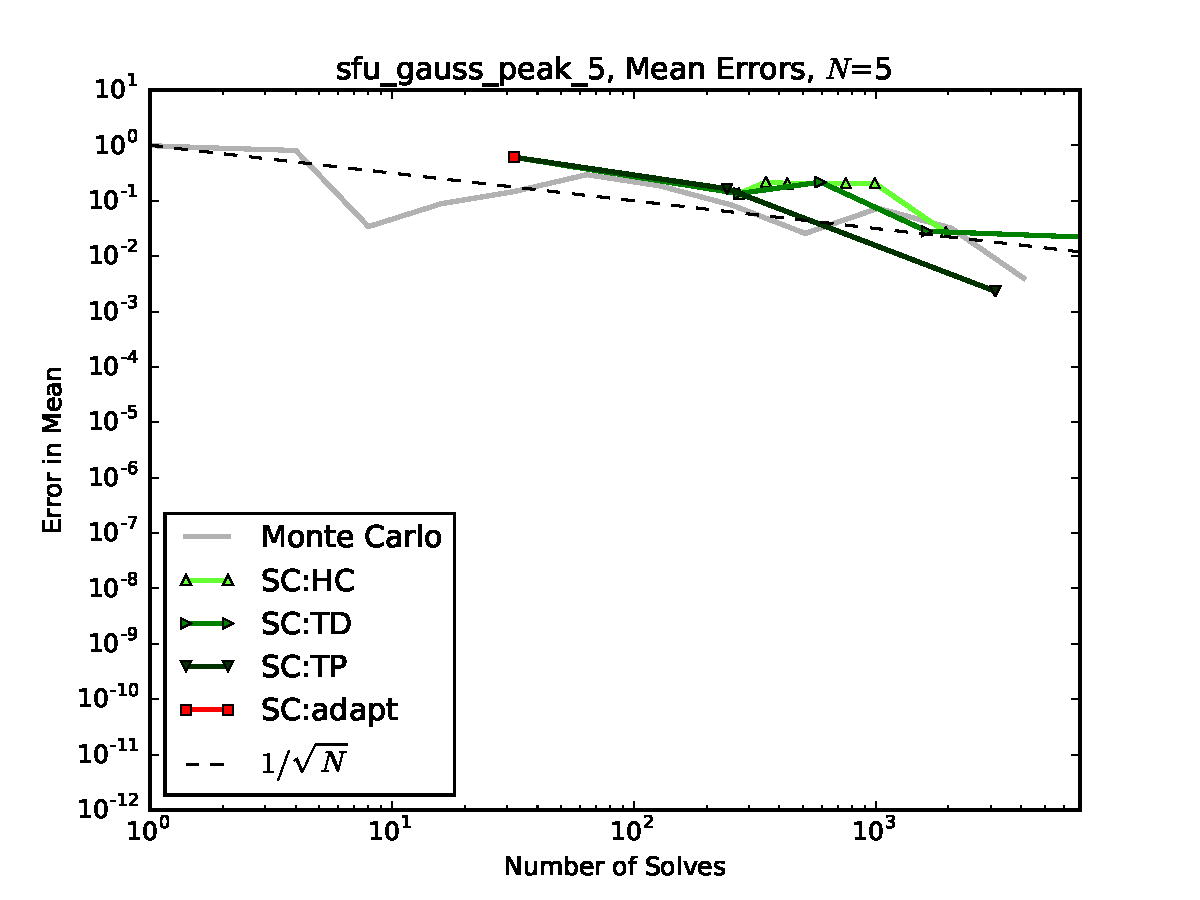
\includegraphics[width=0.8\linewidth]{anlmodels/sfu_gauss_peak_5_mean_errs_nohdmr}
        \end{figure}
        \vspace{-20pt}
        \begin{figure}[h!]
          \centering
          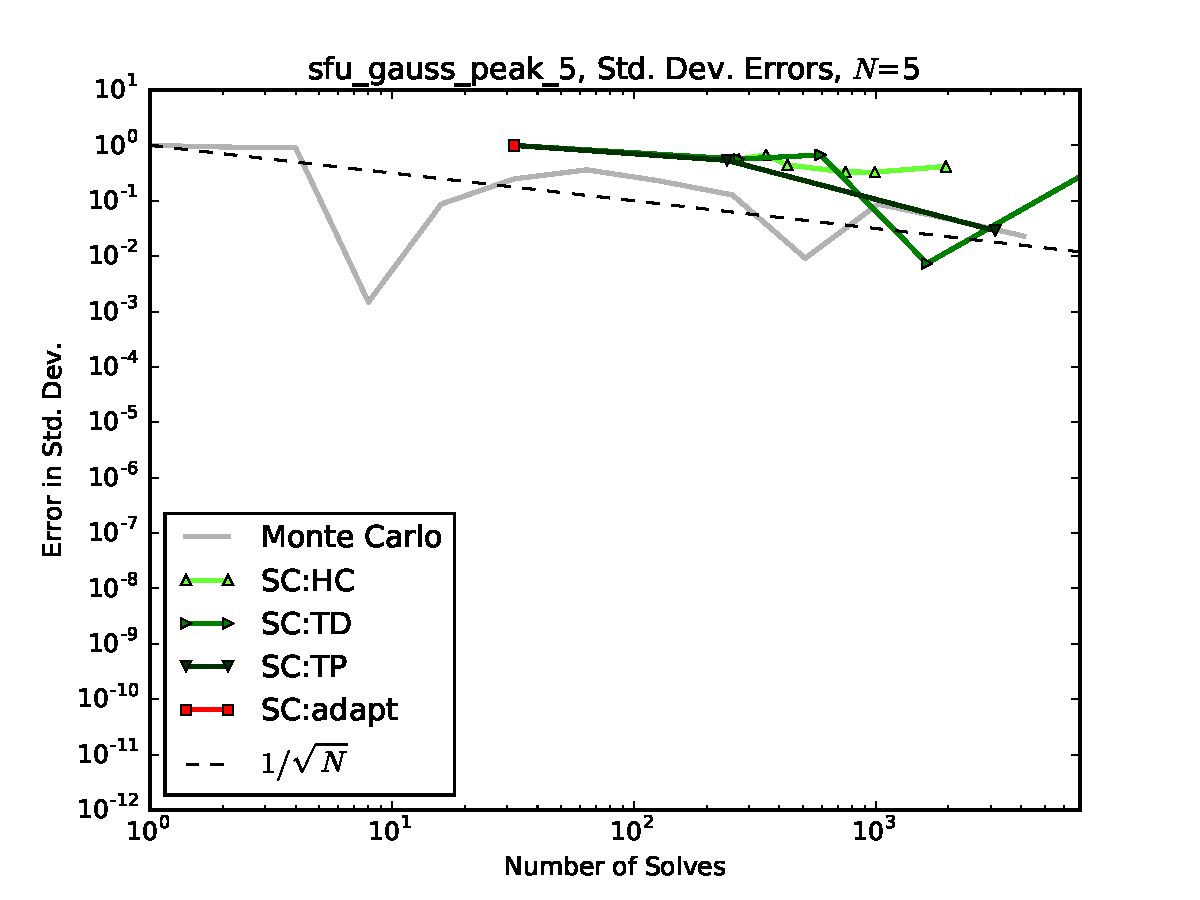
\includegraphics[width=0.8\linewidth]{anlmodels/sfu_gauss_peak_5_variance_errs_nohdmr}
        \end{figure}
   \end{column}
 \end{columns}
\end{frame}


\subsubsection{Ishigami}
\begin{frame}{SCgPC Results}{Ishigami Function}\vspace{-20pt}
  \begin{columns}
    \begin{column}{0.6\textwidth}
      \begin{block}{Ishigami Function}
        \[u(Y) = \sin{y_1} + a\sin^2{y_2} + b\ y_3^4\sin{y_1}\]
      \end{block}
    \end{column}
    \begin{column}{0.4\textwidth}
        \begin{figure}[h!]
          \centering
          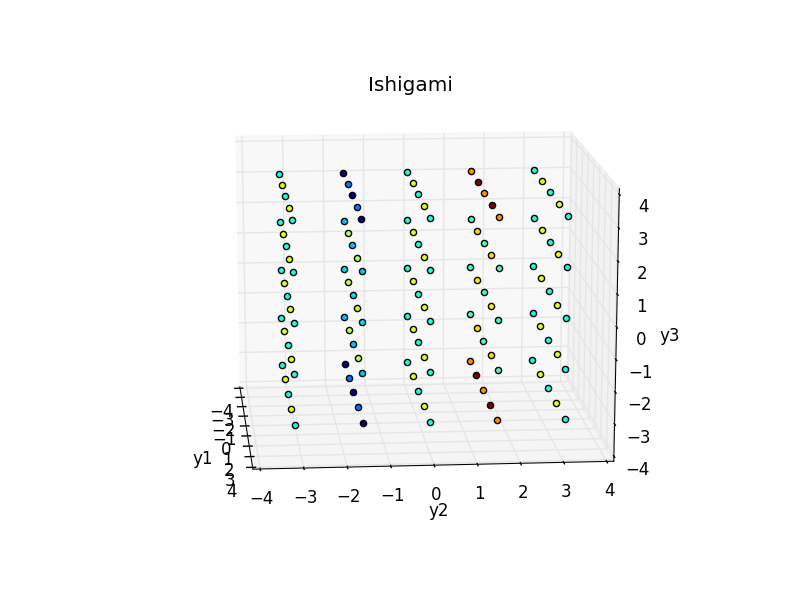
\includegraphics[width=\linewidth]{anlmodels/ishigami}
        \end{figure}
    \end{column}
  \end{columns}
  \begin{itemize}
    \item Not a tensor combination
    \item Strange interplay between $y_1,y_3$
  \end{itemize}
\end{frame}
\begin{frame}{SCgPC Results}{Ishigami Function, Taylor Expansion}\vspace{-20pt}
      \begin{block}{Ishigami Function}
        \[u(Y) = \sin{y_1} + a\sin^2{y_2} + b\ y_3^4\sin{y_1}\]
      \end{block}
\vfill
\begin{equation*}
  \sin{y} = x - \frac{x^3}{6} + \frac{x^5}{120} + \mathcal{O}(x^7)
\end{equation*}
\vfill
\begin{equation*}
  \sin^2{y} = x^2 - \frac{x^4}{3} + \frac{2x^6}{45} + \mathcal{O}(x^8)
\end{equation*}
\vfill
\end{frame}
\begin{frame}{SCgPC Results}{Ishigami Function, $N=3$}\vspace{-20pt}
 \begin{columns}
   \begin{column}{0.5\textwidth}
        \begin{figure}[h!]
          \centering
          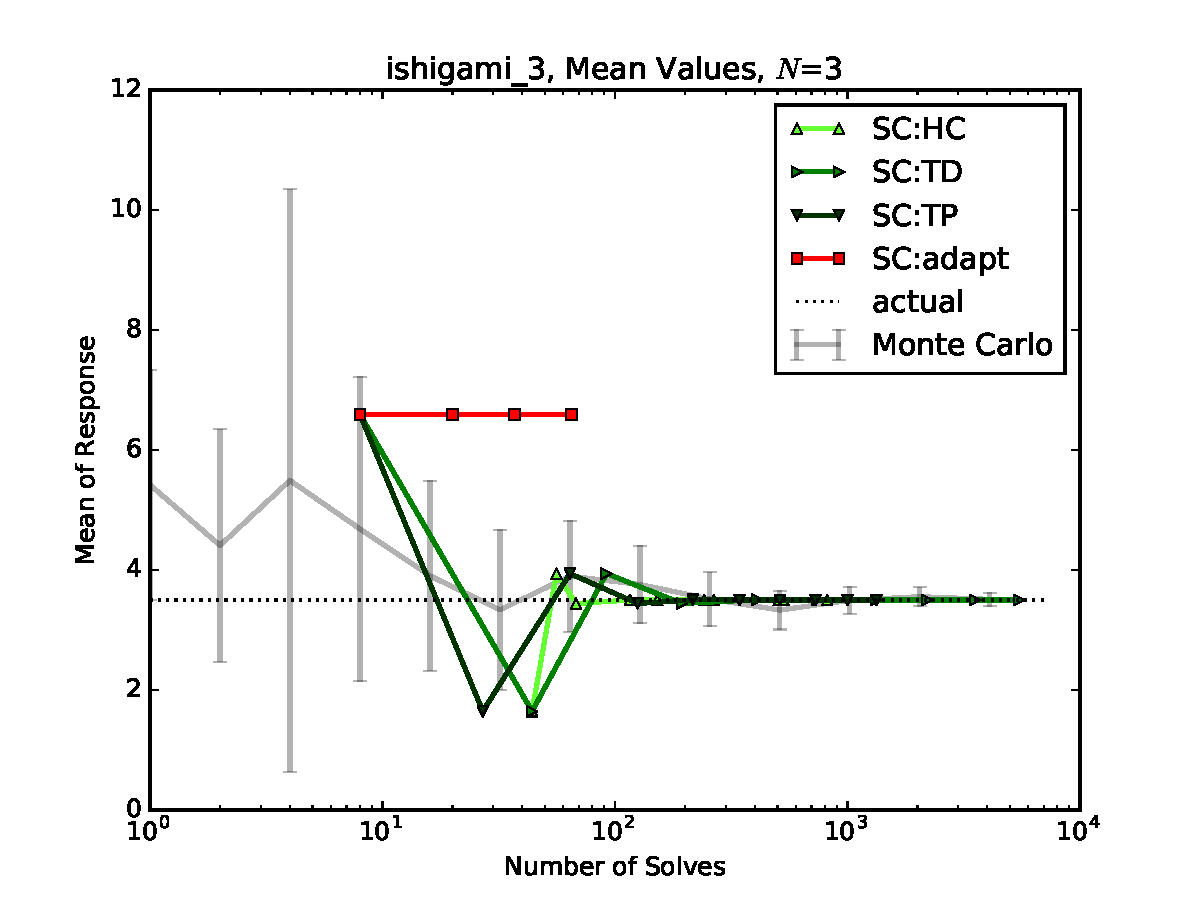
\includegraphics[width=0.8\linewidth]{anlmodels/ishigami_3_mean_vals_nohdmr}
        \end{figure}
        \vspace{-20pt}
        \begin{figure}[h!]
          \centering
          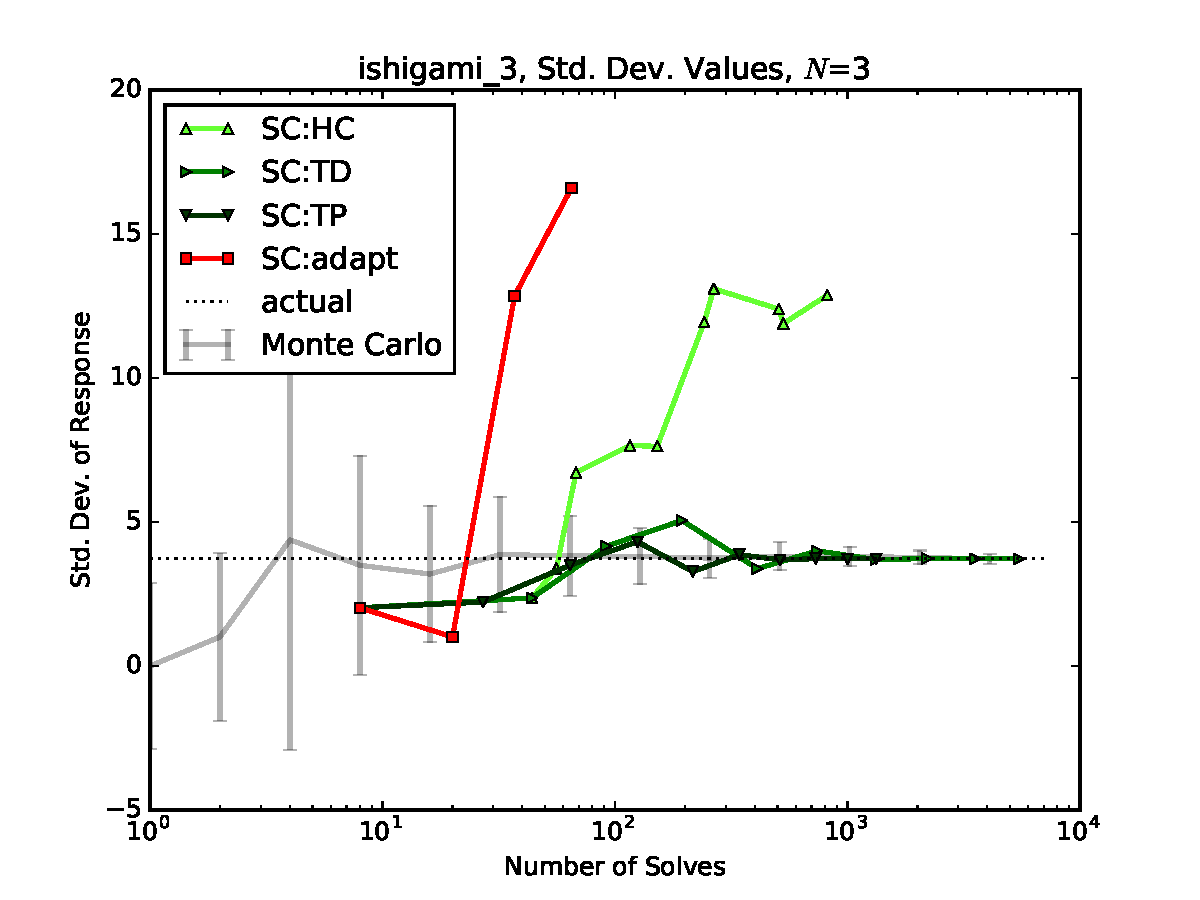
\includegraphics[width=0.8\linewidth]{anlmodels/ishigami_3_var_vals_nohdmr}
        \end{figure}
   \end{column}
   \begin{column}{0.5\textwidth}
        \begin{figure}[h!]
          \centering
          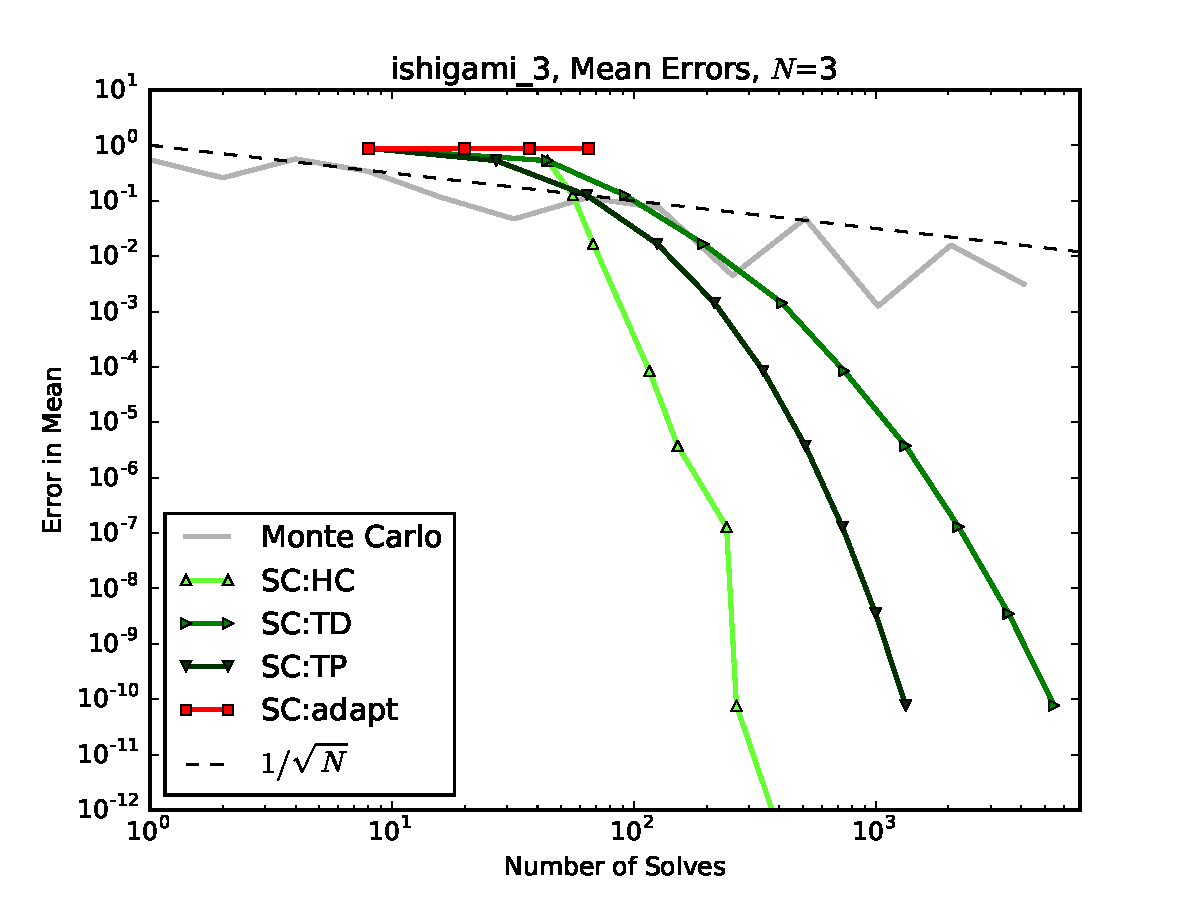
\includegraphics[width=0.8\linewidth]{anlmodels/ishigami_3_mean_errs_nohdmr}
        \end{figure}
        \vspace{-20pt}
        \begin{figure}[h!]
          \centering
          \includegraphics[width=0.8\linewidth]{anlmodels/ishigami_3_variance_errs_nohdmr}
        \end{figure}
   \end{column}
 \end{columns}
\end{frame}




\subsubsection{Sobol G-Function}
\begin{frame}{SCgPC Results}{Sobol G-Function}\vspace{-20pt}
  \begin{columns}
    \begin{column}{0.65\textwidth}
      \begin{block}{Sobol G-Function}
        \[u(Y) = \prod_{n=1}^N \frac{|4y_n-2|-a_n}{1+a_n},\hspace{10pt}a_n=\frac{n-2}{2}\]
      \end{block}
    \end{column}
    \begin{column}{0.35\textwidth}
        \begin{figure}[h!]
          \centering
          \includegraphics[width=\linewidth]{anlmodels/gfunc}
        \end{figure}
    \end{column}
  \end{columns}
  \begin{itemize}
    \item Tensor combination of terms
    \item Only zeroth-order continuity
  \end{itemize}
\end{frame}
\begin{frame}{SCgPC Results}{Sobol G-Function, $N=3$}\vspace{-20pt}
 \begin{columns}
   \begin{column}{0.5\textwidth}
        \begin{figure}[h!]
          \centering
          \includegraphics[width=0.8\linewidth]{anlmodels/sobolG_3_mean_vals_nohdmr}
        \end{figure}
        \vspace{-20pt}
        \begin{figure}[h!]
          \centering
          \includegraphics[width=0.8\linewidth]{anlmodels/sobolG_3_var_vals_nohdmr}
        \end{figure}
   \end{column}
   \begin{column}{0.5\textwidth}
        \begin{figure}[h!]
          \centering
          \includegraphics[width=0.8\linewidth]{anlmodels/sobolG_3_mean_errs_nohdmr}
        \end{figure}
        \vspace{-20pt}
        \begin{figure}[h!]
          \centering
          \includegraphics[width=0.8\linewidth]{anlmodels/sobolG_3_variance_errs_nohdmr}
        \end{figure}
   \end{column}
 \end{columns}
\end{frame}
\begin{frame}{SCgPC Results}{Sobol G-Function, $N=5$}\vspace{-20pt}
 \begin{columns}
   \begin{column}{0.5\textwidth}
        \begin{figure}[h!]
          \centering
          \includegraphics[width=0.8\linewidth]{anlmodels/sobolG_5_mean_vals_nohdmr}
        \end{figure}
        \vspace{-20pt}
        \begin{figure}[h!]
          \centering
          \includegraphics[width=0.8\linewidth]{anlmodels/sobolG_5_var_vals_nohdmr}
        \end{figure}
   \end{column}
   \begin{column}{0.5\textwidth}
        \begin{figure}[h!]
          \centering
          \includegraphics[width=0.8\linewidth]{anlmodels/sobolG_5_mean_errs_nohdmr}
        \end{figure}
        \vspace{-20pt}
        \begin{figure}[h!]
          \centering
          \includegraphics[width=0.8\linewidth]{anlmodels/sobolG_5_variance_errs_nohdmr}
        \end{figure}
   \end{column}
 \end{columns}
\end{frame}



%\subsection{SCgPC Conclusions}
\begin{frame}{SCgPC Results}{Conclusions}\vspace{-20pt}
  \vfill
Regarding static SCgPC:
\begin{itemize}
  \item Great in low input space dimensionality
  \item Better with regular responses
  \item Total Degree often great choice
\end{itemize}
  \vfill
Regarding adaptive SCgPC:
\begin{itemize}
  \item Optimal for small input dimensionality
  \item Monotonically-decreasing variance moments
  \item Very poor if oscillating moments
\end{itemize}
  \vfill
\end{frame}

\section{HDMR Results}
\subsubsection{Tensor Monomials}
\begin{frame}{HDMR Results}{Tensor Monomials}\vspace{-20pt}
  \begin{columns}
    \begin{column}{0.6\textwidth}
      \begin{block}{Tensor Monomials}
        \[u(Y) = \prod_{n=1}^N (y_n+1)\]
      \end{block}
    \end{column}
    \begin{column}{0.4\textwidth}
        \begin{figure}[h!]
          \centering
          \includegraphics[width=\linewidth]{anlmodels/tensor_monom}
        \end{figure}
    \end{column}
  \end{columns}
  \begin{itemize}
    \item Linear response
    \item All polynomial combinations
  \end{itemize}
\end{frame}
\begin{frame}{HDMR Results}{Tensor Monomials, $N=3$}\vspace{-20pt}
 \begin{columns}
   \begin{column}{0.5\textwidth}
        \begin{figure}[h!]
          \centering
          \includegraphics[width=0.8\linewidth]{anlmodels/tensor_monomial_3_mean_vals}
        \end{figure}
        \vspace{-20pt}
        \begin{figure}[h!]
          \centering
          \includegraphics[width=0.8\linewidth]{anlmodels/tensor_monomial_3_var_vals}
        \end{figure}
   \end{column}
   \begin{column}{0.5\textwidth}
        \begin{figure}[h!]
          \centering
          \includegraphics[width=0.8\linewidth]{anlmodels/tensor_monomial_3_mean_errs}
        \end{figure}
        \vspace{-20pt}
        \begin{figure}[h!]
          \centering
          \includegraphics[width=0.8\linewidth]{anlmodels/tensor_monomial_3_variance_errs}
        \end{figure}
   \end{column}
 \end{columns}
\end{frame}
\begin{frame}{HDMR Results}{Tensor Monomials, $N=5$}\vspace{-20pt}
 \begin{columns}
   \begin{column}{0.5\textwidth}
        \begin{figure}[h!]
          \centering
          \includegraphics[width=0.8\linewidth]{anlmodels/tensor_monomial_5_mean_vals}
        \end{figure}
        \vspace{-20pt}
        \begin{figure}[h!]
          \centering
          \includegraphics[width=0.8\linewidth]{anlmodels/tensor_monomial_5_var_vals}
        \end{figure}
   \end{column}
   \begin{column}{0.5\textwidth}
        \begin{figure}[h!]
          \centering
          \includegraphics[width=0.8\linewidth]{anlmodels/tensor_monomial_5_mean_errs}
        \end{figure}
        \vspace{-20pt}
        \begin{figure}[h!]
          \centering
          \includegraphics[width=0.8\linewidth]{anlmodels/tensor_monomial_5_variance_errs}
        \end{figure}
   \end{column}
 \end{columns}
\end{frame}
\begin{frame}{HDMR Results}{Tensor Monomials, $N=10$}\vspace{-20pt}
 \begin{columns}
   \begin{column}{0.5\textwidth}
        \begin{figure}[h!]
          \centering
          \includegraphics[width=0.8\linewidth]{anlmodels/tensor_monomial_10_mean_vals}
        \end{figure}
        \vspace{-20pt}
        \begin{figure}[h!]
          \centering
          \includegraphics[width=0.8\linewidth]{anlmodels/tensor_monomial_10_var_vals}
        \end{figure}
   \end{column}
   \begin{column}{0.5\textwidth}
        \begin{figure}[h!]
          \centering
          \includegraphics[width=0.8\linewidth]{anlmodels/tensor_monomial_10_mean_errs}
        \end{figure}
        \vspace{-20pt}
        \begin{figure}[h!]
          \centering
          \includegraphics[width=0.8\linewidth]{anlmodels/tensor_monomial_10_variance_errs}
        \end{figure}
   \end{column}
 \end{columns}
\end{frame}



\subsubsection{Sudret Polynomial}
\begin{frame}{HDMR Results}{Sudret Polynomials}\vspace{-20pt}
  \begin{columns}
    \begin{column}{0.6\textwidth}
      \begin{block}{Sudret Polynomials}
        \[u(Y) = \frac{1}{2^N}\prod_{n=1}^N (3y_n^2+1)\]
      \end{block}
    \end{column}
    \begin{column}{0.4\textwidth}
        \begin{figure}[h!]
          \centering
          \includegraphics[width=\linewidth]{anlmodels/sudret}
        \end{figure}
    \end{column}
  \end{columns}
  \begin{itemize}
    \item Exclusively second-order interactions
    \item All second-order polynomial combinations
  \end{itemize}
\end{frame}
\begin{frame}{HDMR Results}{Sudret Polynomials, $N=3$}\vspace{-20pt}
 \begin{columns}
   \begin{column}{0.5\textwidth}
        \begin{figure}[h!]
          \centering
          \includegraphics[width=0.8\linewidth]{anlmodels/sudret_3_mean_vals}
        \end{figure}
        \vspace{-20pt}
        \begin{figure}[h!]
          \centering
          \includegraphics[width=0.8\linewidth]{anlmodels/sudret_3_var_vals}
        \end{figure}
   \end{column}
   \begin{column}{0.5\textwidth}
        \begin{figure}[h!]
          \centering
          \includegraphics[width=0.8\linewidth]{anlmodels/sudret_3_mean_errs}
        \end{figure}
        \vspace{-20pt}
        \begin{figure}[h!]
          \centering
          \includegraphics[width=0.8\linewidth]{anlmodels/sudret_3_variance_errs}
        \end{figure}
   \end{column}
 \end{columns}
\end{frame}
\begin{frame}{HDMR Results}{Sudret Polynomials, $N=5$}\vspace{-20pt}
 \begin{columns}
   \begin{column}{0.5\textwidth}
        \begin{figure}[h!]
          \centering
          \includegraphics[width=0.8\linewidth]{anlmodels/sudret_5_mean_vals}
        \end{figure}
        \vspace{-20pt}
        \begin{figure}[h!]
          \centering
          \includegraphics[width=0.8\linewidth]{anlmodels/sudret_5_var_vals}
        \end{figure}
   \end{column}
   \begin{column}{0.5\textwidth}
        \begin{figure}[h!]
          \centering
          \includegraphics[width=0.8\linewidth]{anlmodels/sudret_5_mean_errs}
        \end{figure}
        \vspace{-20pt}
        \begin{figure}[h!]
          \centering
          \includegraphics[width=0.8\linewidth]{anlmodels/sudret_5_variance_errs}
        \end{figure}
   \end{column}
 \end{columns}
\end{frame}


\subsubsection{Attenuation}
\begin{frame}{HDMR Results}{Attenuation}\vspace{-20pt}
  \begin{columns}
    \begin{column}{0.6\textwidth}
      \begin{block}{Attenuation}
        \[u(Y) = \prod_{n=1}^N \exp(-y_n/N)\]
      \end{block}
    \end{column}
    \begin{column}{0.4\textwidth}
        \begin{figure}[h!]
          \centering
          \includegraphics[width=\linewidth]{anlmodels/attenuate}
        \end{figure}
    \end{column}
  \end{columns}
  \begin{itemize}
    \item Tensor of decreasing-importance polynomials
    \item Combination terms over single-variable
  \end{itemize}
\end{frame}
\begin{frame}{HDMR Results}{Attenuation, Taylor Expansion}%\vspace{-20pt}
  \begin{equation*}
    e^{-ay} = 1 - ay + \frac{(ay)^2}{2} - \frac{(ay)^3}{6} + \frac{(ay)^4}{24} - \frac{(ay)^5}{120} +
          \mathcal{O}(y^6)
  \end{equation*}
\begin{table}
  \centering
  \begin{tabular}{|c c|c c c c c|}
    \cline{3-7}\multicolumn{2}{c|}{ } & \multicolumn{5}{c|}{Polynomial Order ($y_1$)} \\
               \multicolumn{2}{c|}{ } & 0 & 1 & 2 & 3 & 4 \\
    \hline & 0 & 1        & $a$      & $a^2/2$  & $a^3/6$   & \cellcolor{Gray6}$a^4/24$  \\
Polynomial & 1 & $a$      & $a^2   $ & $a^3/2 $ & \cellcolor{Gray6}$a^4/6  $ & $a^5/24 $ \\
Order      & 2 & $a^2/2$  & $a^3/2 $ & \cellcolor{Gray6}$a^4/4 $ & $a^5/12 $ & $a^6/48 $ \\
($y_2$)    & 3 & $a^3/ 6$ & \cellcolor{Gray6}$a^4/ 6$ & $a^5/12$ & $a^6/ 36$ & $a^7/144$ \\
           & 4 & \cellcolor{Gray6}$a^4/24$ & $a^5/24$ & $a^6/48$ & $a^7/144$ & $a^8/576$ \\
    \hline
  \end{tabular}
\end{table}
\end{frame}
\begin{frame}{HDMR Results}{Attenuation, $N=2$}\vspace{-20pt}
 \begin{columns}
   \begin{column}{0.5\textwidth}
        \begin{figure}[h!]
          \centering
          \includegraphics[width=0.8\linewidth]{anlmodels/attenuate_2_mean_vals}
        \end{figure}
        \vspace{-20pt}
        \begin{figure}[h!]
          \centering
          \includegraphics[width=0.8\linewidth]{anlmodels/attenuate_2_var_vals}
        \end{figure}
   \end{column}
   \begin{column}{0.5\textwidth}
        \begin{figure}[h!]
          \centering
          \includegraphics[width=0.8\linewidth]{anlmodels/attenuate_2_mean_errs}
        \end{figure}
        \vspace{-20pt}
        \begin{figure}[h!]
          \centering
          \includegraphics[width=0.8\linewidth]{anlmodels/attenuate_2_variance_errs}
        \end{figure}
   \end{column}
 \end{columns}
\end{frame}
\begin{frame}{HDMR Results}{Attenuation, $N=4$}\vspace{-20pt}
 \begin{columns}
   \begin{column}{0.5\textwidth}
        \begin{figure}[h!]
          \centering
          \includegraphics[width=0.8\linewidth]{anlmodels/attenuate_4_mean_vals}
        \end{figure}
        \vspace{-20pt}
        \begin{figure}[h!]
          \centering
          \includegraphics[width=0.8\linewidth]{anlmodels/attenuate_4_var_vals}
        \end{figure}
   \end{column}
   \begin{column}{0.5\textwidth}
        \begin{figure}[h!]
          \centering
          \includegraphics[width=0.8\linewidth]{anlmodels/attenuate_4_mean_errs}
        \end{figure}
        \vspace{-20pt}
        \begin{figure}[h!]
          \centering
          \includegraphics[width=0.8\linewidth]{anlmodels/attenuate_4_variance_errs}
        \end{figure}
   \end{column}
 \end{columns}
\end{frame}
\begin{frame}{HDMR Results}{Attenuation, $N=6$}\vspace{-20pt}
 \begin{columns}
   \begin{column}{0.5\textwidth}
        \begin{figure}[h!]
          \centering
          \includegraphics[width=0.8\linewidth]{anlmodels/attenuate_6_mean_vals}
        \end{figure}
        \vspace{-20pt}
        \begin{figure}[h!]
          \centering
          \includegraphics[width=0.8\linewidth]{anlmodels/attenuate_6_var_vals}
        \end{figure}
   \end{column}
   \begin{column}{0.5\textwidth}
        \begin{figure}[h!]
          \centering
          \includegraphics[width=0.8\linewidth]{anlmodels/attenuate_6_mean_errs}
        \end{figure}
        \vspace{-20pt}
        \begin{figure}[h!]
          \centering
          \includegraphics[width=0.8\linewidth]{anlmodels/attenuate_6_variance_errs}
        \end{figure}
   \end{column}
 \end{columns}
\end{frame}




\subsubsection{Gauss Peak}
\begin{frame}{HDMR Results}{Gauss Peak}\vspace{-20pt}
  \begin{columns}
    \begin{column}{0.6\textwidth}
      \begin{block}{Gauss Peak}
        \[u(Y) = \prod_{n=1}^N \exp(-3^2(y_n-0.5)^2)\]
      \end{block}
    \end{column}
    \begin{column}{0.4\textwidth}
        \begin{figure}[h!]
          \centering
          \includegraphics[width=\linewidth]{anlmodels/gaussian}
        \end{figure}
    \end{column}
  \end{columns}
  \begin{itemize}
    \item Tensor of polynomials
    \item Slow, inconsistent decay
  \end{itemize}
\end{frame}
\begin{frame}{HDMR Results}{Gauss Peak, Taylor Expansion}\vspace{-20pt}
\begin{equation*}
  e^{-a^2y^2} = 1 - a^2y^2 + \frac{a^4}{2}y^4 - \frac{a^6}{6}y^6 + \frac{a^8}{24}y^8 + \mathcal{O}(y^{10})
\end{equation*}
\begin{table}
  \centering
  \begin{tabular}{|c c|c c c c c|}
    \cline{3-7}\multicolumn{2}{c|}{ } & \multicolumn{5}{c|}{Polynomial Order ($y_1$)} \\
\multicolumn{2}{c|}{ } & 0       & 1 & 2       & 3 & 4       \\
    \hline         & 0 & 1       & 0 & $a^2$   & 0 & $a^4/2$ \\
Polynomial         & 1 & 0       & 0 & 0       & 0 & 0       \\
Order              & 2 & $a^2$   & 0 & $a^4$   & 0 & $a^6/2$ \\
($y_2$)            & 3 & 0       & 0 & 0       & 0 & 0       \\
                   & 4 & $a^4/2$ & 0 & $a^6/2$ & 0 & $a^8/4$ \\
    \hline
  \end{tabular}
\end{table}
\end{frame}
\begin{frame}{HDMR Results}{Gauss Peak, $N=3$}\vspace{-20pt}
 \begin{columns}
   \begin{column}{0.5\textwidth}
        \begin{figure}[h!]
          \centering
          \includegraphics[width=0.8\linewidth]{anlmodels/sfu_gauss_peak_3_mean_vals}
        \end{figure}
        \vspace{-20pt}
        \begin{figure}[h!]
          \centering
          \includegraphics[width=0.8\linewidth]{anlmodels/sfu_gauss_peak_3_var_vals}
        \end{figure}
   \end{column}
   \begin{column}{0.5\textwidth}
        \begin{figure}[h!]
          \centering
          \includegraphics[width=0.8\linewidth]{anlmodels/sfu_gauss_peak_3_mean_errs}
        \end{figure}
        \vspace{-20pt}
        \begin{figure}[h!]
          \centering
          \includegraphics[width=0.8\linewidth]{anlmodels/sfu_gauss_peak_3_variance_errs}
        \end{figure}
   \end{column}
 \end{columns}
\end{frame}
\begin{frame}{HDMR Results}{Gauss Peak, $N=5$}\vspace{-20pt}
 \begin{columns}
   \begin{column}{0.5\textwidth}
        \begin{figure}[h!]
          \centering
          \includegraphics[width=0.8\linewidth]{anlmodels/sfu_gauss_peak_5_mean_vals}
        \end{figure}
        \vspace{-20pt}
        \begin{figure}[h!]
          \centering
          \includegraphics[width=0.8\linewidth]{anlmodels/sfu_gauss_peak_5_var_vals}
        \end{figure}
   \end{column}
   \begin{column}{0.5\textwidth}
        \begin{figure}[h!]
          \centering
          \includegraphics[width=0.8\linewidth]{anlmodels/sfu_gauss_peak_5_mean_errs}
        \end{figure}
        \vspace{-20pt}
        \begin{figure}[h!]
          \centering
          \includegraphics[width=0.8\linewidth]{anlmodels/sfu_gauss_peak_5_variance_errs}
        \end{figure}
   \end{column}
 \end{columns}
\end{frame}


\subsubsection{Ishigami}
\begin{frame}{HDMR Results}{Ishigami Function}\vspace{-20pt}
  \begin{columns}
    \begin{column}{0.6\textwidth}
      \begin{block}{Ishigami Function}
        \[u(Y) = \sin{y_1} + a\sin^2{y_2} + b\ y_3^4\sin{y_1}\]
      \end{block}
    \end{column}
    \begin{column}{0.4\textwidth}
        \begin{figure}[h!]
          \centering
          \includegraphics[width=\linewidth]{anlmodels/ishigami}
        \end{figure}
    \end{column}
  \end{columns}
  \begin{itemize}
    \item Not a tensor combination
    \item Strange interplay between $y_1,y_3$
  \end{itemize}
\end{frame}
\begin{frame}{HDMR Results}{Ishigami Function, Taylor Expansion}\vspace{-20pt}
      \begin{block}{Ishigami Function}
        \[u(Y) = \sin{y_1} + a\sin^2{y_2} + b\ y_3^4\sin{y_1}\]
      \end{block}
\vfill
\begin{equation*}
  \sin{y} = x - \frac{x^3}{6} + \frac{x^5}{120} + \mathcal{O}(x^7)
\end{equation*}
\vfill
\begin{equation*}
  \sin^2{y} = x^2 - \frac{x^4}{3} + \frac{2x^6}{45} + \mathcal{O}(x^8)
\end{equation*}
\vfill
\end{frame}
\begin{frame}{HDMR Results}{Ishigami Function, $N=3$}\vspace{-20pt}
 \begin{columns}
   \begin{column}{0.5\textwidth}
        \begin{figure}[h!]
          \centering
          \includegraphics[width=0.8\linewidth]{anlmodels/ishigami_3_mean_vals}
        \end{figure}
        \vspace{-20pt}
        \begin{figure}[h!]
          \centering
          \includegraphics[width=0.8\linewidth]{anlmodels/ishigami_3_var_vals}
        \end{figure}
   \end{column}
   \begin{column}{0.5\textwidth}
        \begin{figure}[h!]
          \centering
          \includegraphics[width=0.8\linewidth]{anlmodels/ishigami_3_mean_errs}
        \end{figure}
        \vspace{-20pt}
        \begin{figure}[h!]
          \centering
          \includegraphics[width=0.8\linewidth]{anlmodels/ishigami_3_variance_errs}
        \end{figure}
   \end{column}
 \end{columns}
\end{frame}




\subsubsection{Sobol G-Function}
\begin{frame}{HDMR Results}{Sobol G-Function}\vspace{-20pt}
  \begin{columns}
    \begin{column}{0.65\textwidth}
      \begin{block}{Sobol G-Function}
        \[u(Y) = \prod_{n=1}^N \frac{|4y_n-2|-a_n}{1+a_n},\hspace{10pt}a_n=\frac{n-2}{2}\]
      \end{block}
    \end{column}
    \begin{column}{0.35\textwidth}
        \begin{figure}[h!]
          \centering
          \includegraphics[width=\linewidth]{anlmodels/gfunc}
        \end{figure}
    \end{column}
  \end{columns}
  \begin{itemize}
    \item Tensor combination of terms
    \item Only zeroth-order continuity
  \end{itemize}
\end{frame}
\begin{frame}{HDMR Results}{Sobol G-Function, $N=3$}\vspace{-20pt}
 \begin{columns}
   \begin{column}{0.5\textwidth}
        \begin{figure}[h!]
          \centering
          \includegraphics[width=0.8\linewidth]{anlmodels/sobolG_3_mean_vals}
        \end{figure}
        \vspace{-20pt}
        \begin{figure}[h!]
          \centering
          \includegraphics[width=0.8\linewidth]{anlmodels/sobolG_3_var_vals}
        \end{figure}
   \end{column}
   \begin{column}{0.5\textwidth}
        \begin{figure}[h!]
          \centering
          \includegraphics[width=0.8\linewidth]{anlmodels/sobolG_3_mean_errs}
        \end{figure}
        \vspace{-20pt}
        \begin{figure}[h!]
          \centering
          \includegraphics[width=0.8\linewidth]{anlmodels/sobolG_3_variance_errs}
        \end{figure}
   \end{column}
 \end{columns}
\end{frame}
\begin{frame}{HDMR Results}{Sobol G-Function, $N=5$}\vspace{-20pt}
 \begin{columns}
   \begin{column}{0.5\textwidth}
        \begin{figure}[h!]
          \centering
          \includegraphics[width=0.8\linewidth]{anlmodels/sobolG_5_mean_vals}
        \end{figure}
        \vspace{-20pt}
        \begin{figure}[h!]
          \centering
          \includegraphics[width=0.8\linewidth]{anlmodels/sobolG_5_var_vals}
        \end{figure}
   \end{column}
   \begin{column}{0.5\textwidth}
        \begin{figure}[h!]
          \centering
          \includegraphics[width=0.8\linewidth]{anlmodels/sobolG_5_mean_errs}
        \end{figure}
        \vspace{-20pt}
        \begin{figure}[h!]
          \centering
          \includegraphics[width=0.8\linewidth]{anlmodels/sobolG_5_variance_errs}
        \end{figure}
   \end{column}
 \end{columns}
\end{frame}



%\subsection{HDMR Conclusions}
\begin{frame}{HDMR Results}{Conclusions}\vspace{-20pt}
  \vfill
Regarding static HDMR:
\begin{itemize}
  \item Never outperforms associated SCgPC
  \item Does produce results with less evaluations
\end{itemize}
  \vfill
Regarding adaptive HDMR:
\begin{itemize}
  \item Sometimes outperforms adaptive SCgPC
  \item Yields results with fewer evaluations
\end{itemize}
  \vfill
HDMR is most useful when very few evaluations possible
  \vfill
\end{frame}




\section{Neutronics Example}
\subsection{Problem}
\begin{frame}{Neutronics Example}{Introduction}\vspace{-20pt}
  More complicated than an analytic case
\begin{align*}
  -D_g(\mathbf{r})\nabla^2\phi_g(\mathbf{r}) + \Sigma_{a,g}(\mathbf{r}) &=
           \sum_{g'=1}^G \Sigma_{g'\to g}\phi_{g'}(\mathbf{r})\\
  & +\frac{\chi_{p,g}}{k}\sum_{g'=1}^G \nu\Sigma_{f,g'}(\mathbf{r})\phi_{g'}(\mathbf{r})
\end{align*}
  Quantities of interest
  \begin{itemize}
    \item $\phi_g(\mathbf{r})$: Group neutron flux
    \item $k$ eigenvalue: Neutron multiplication factor
  \end{itemize}
\end{frame}

\begin{frame}{Neutronics Example}{Geometry}%\vspace{-20pt}
  \vfill
  Quarter-symmetric 4-assembly reactor core
  \vfill
  \begin{figure}
    \centering
    \includegraphics[width=0.5\linewidth]{c5g7/geom}
  \end{figure}
  \vfill
\end{frame}

\begin{frame}{Neutronics Example}{Energy Groups}%\vspace{-20pt}
7 energy groups, 7 materials, 32 mesh elements per pin
  \begin{table}
    \centering{}
    \begin{tabular}{c c}
      Group & Upper Energy Bound \\ \hline
      7 & 0.02 eV\\
      6 & 0.1 eV\\
      5 & 0.625 eV\\
      4 & 3 eV\\
      3 & 500 keV \\
      2 & 1 MeV \\
      1 & 20 MeV
    \end{tabular}
  \end{table}
Solved using \texttt{RATTLESNAKE}'s linear CFEM
\end{frame}

\begin{frame}{Neutronics Example}{Flux Profiles}%\vspace{-20pt}
  \begin{columns}
    \begin{column}{0.5\textwidth}
      \begin{figure}
        \centering
        \includegraphics[width=\linewidth]{c5g7/flux0}
      \end{figure}
    \end{column}
    \begin{column}{0.5\textwidth}
      \begin{figure}
        \centering
        \includegraphics[width=\linewidth]{c5g7/flux5}
      \end{figure}
    \end{column}
  \end{columns}
\end{frame}



\subsection{Uncertainty}
\begin{frame}{Neutronics Example}{Uncertainty}%\vspace{-20pt}
  \vfill
  Specific Responses
  \begin{itemize}
    \item $k$-eigenvalue
    \item Group 1 flux at reactor center
    \item Group 5 flux at reactor center
  \end{itemize}
  \vfill
  168 correlated uncertain inputs
  \begin{itemize}
    \item Material macroscopic cross sections
    \item Assigned 10\% correlation
      \begin{itemize}
        \item Same material and reaction, different energies
        \item Same material and energy, different reaction
      \end{itemize}
    \item Relative variance of 5\% for all inputs
  \end{itemize}
  \vfill
\end{frame}

\begin{frame}{Neutronics Example}{Uncertainty Correlations}\vspace{-20pt}
  \vfill
  Need to de-correlate input space
  \vfill
  \raven{} has two-step reduction
  \begin{itemize}
    \item Karhunen-Loeve expansion (PCA)
    \item Sensitivity reduction
    \item Combined yields \emph{importance rank}
  \end{itemize}
  \vfill
\end{frame}

\begin{frame}{Neutronics Example}{Uncertainty Correlations}\vspace{-20pt}
\begin{table}
\tiny
  \centering \hspace{-20pt}
  \begin{tabular}{|c|c c|c c|c c|} \hline
    & \multicolumn{2}{|c|}{$k$-eigenvalue} & \multicolumn{2}{|c|}{Center Flux, $g=1$} &
             \multicolumn{2}{|c|}{Center Flux, $g=5$} \\ \hline
    Rank & Dimension & Importance & Dimension & Importance & Dimension & Importance \\ \hline
    1 &  24 & 0.09606 &  24 & 0.07231 &  24 &  0.07032  \\
    2 &   9 & 0.08555 &   9 & 0.06472 &   9 &  0.06648  \\
    3 &   0 & 0.06861 &   0 & 0.04856 & 100 &  0.06474  \\
    4 &  17 & 0.04737 & 116 & 0.03472 &  13 &  0.03396  \\ \cline{2-3}
    5 &  23 & 0.03415 &  17 & 0.03470 &   0 &  0.03092  \\ 
    6 & 158 & 0.03047 &  10 & 0.02726 &  17 &  0.02716  \\ \cline{4-5}
    7 & 164 & 0.02852 &   8 & 0.02468 &  10 &  0.02651  \\ \cline{6-7}
    8 &  50 & 0.02695 & 164 & 0.02174 & 118 &  0.02600  \\
    9 &   6 & 0.02315 &  20 & 0.02157 & 117 &  0.02420  \\
  \hline \end{tabular}
\end{table}
Retained latent dimensions 24, 9, 0, 17, 10, 116, 100, 13
\end{frame}

\begin{frame}{Neutronics Example}{Uncertainty Correlations}\vspace{-20pt}
  \begin{columns}
    \begin{column}{0.5\textwidth}
      \begin{figure}
        \centering
        \includegraphics[width=0.8\linewidth]{c5g7/C5G7_eigenvalue_impranks}
      \end{figure}
    \end{column}
    \begin{column}{0.5\textwidth}
      \begin{itemize}
        \item Truncated after gradients
        \item Some importance lost
        \item Mean preserved well
        \item Std dev partially preserved
      \end{itemize}
    \end{column}
  \end{columns}
  \begin{columns}
    \begin{column}{0.5\textwidth}
      \begin{figure}
        \centering
        \includegraphics[width=0.8\linewidth]{c5g7/C5G7_center_flux_0_impranks}
      \end{figure}
    \end{column}
    \begin{column}{0.5\textwidth}
      \begin{figure}
        \centering
        \includegraphics[width=0.8\linewidth]{c5g7/C5G7_center_flux_5_impranks}
      \end{figure}
    \end{column}
  \end{columns}
\end{frame}

\begin{frame}{Neutronics Example}{Uncertainty Correlations}\vspace{-20pt}
  \begin{columns}
    \begin{column}{0.3\textwidth}
      \centering
      \vfill
      $k$-Eigenvalue
      \vfill
    \end{column}
    \begin{column}{0.7\textwidth}
      \begin{figure}
        \centering
        \includegraphics[width=\linewidth]{c5g7/C5G7_eigenvalue_mean_reduction}
      \end{figure}
      \vspace{-30pt}
      \begin{figure}
        \centering
        \includegraphics[width=\linewidth]{c5g7/C5G7_eigenvalue_stddev_reduction}
      \end{figure}
    \end{column}
  \end{columns}
\end{frame}
\begin{frame}{Neutronics Example}{Uncertainty Correlations}\vspace{-20pt}
  \begin{columns}
    \begin{column}{0.3\textwidth}
      \centering
      \vfill
      Center Flux, $g=1$
      \vfill
    \end{column}
    \begin{column}{0.7\textwidth}
      \begin{figure}
        \centering
        \includegraphics[width=\linewidth]{c5g7/C5G7_center_flux_g0_mean_reduction}
      \end{figure}
      \vspace{-30pt}
      \begin{figure}
        \centering
        \includegraphics[width=\linewidth]{c5g7/C5G7_center_flux_g0_stddev_reduction}
      \end{figure}
    \end{column}
  \end{columns}
\end{frame}
\begin{frame}{Neutronics Example}{Uncertainty Correlations}\vspace{-20pt}
  \begin{columns}
    \begin{column}{0.3\textwidth}
      \centering
      \vfill
      Center Flux, $g=5$
      \vfill
    \end{column}
    \begin{column}{0.7\textwidth}
      \begin{figure}
        \centering
        \includegraphics[width=\linewidth]{c5g7/C5G7_center_flux_g5_mean_reduction}
      \end{figure}
      \vspace{-30pt}
      \begin{figure}
        \centering
        \includegraphics[width=\linewidth]{c5g7/C5G7_center_flux_g5_stddev_reduction}
      \end{figure}
    \end{column}
  \end{columns}
\end{frame}





\subsection{Results}
\begin{frame}{Neutronics Example}{Results: $k$-eigenvalue}%\vspace{-20pt}
  \begin{columns}
    \begin{column}{0.5\textwidth}
      \begin{figure}
        \centering
        \includegraphics[width=\linewidth]{c5g7/C5G7_eigenvalue_mean_vals}
      \end{figure}
    \end{column}
    \begin{column}{0.5\textwidth}
      \begin{figure}
        \centering
        \includegraphics[width=\linewidth]{c5g7/C5G7_eigenvalue_var_vals}
      \end{figure}
    \end{column}
  \end{columns}
\end{frame}
\begin{frame}{Neutronics Example}{Results: Center Flux, $g=1$}%\vspace{-20pt}
  \begin{columns}
    \begin{column}{0.5\textwidth}
      \begin{figure}
        \centering
        \includegraphics[width=\linewidth]{c5g7/C5G7_center_flux_g0_mean_vals}
      \end{figure}
    \end{column}
    \begin{column}{0.5\textwidth}
      \begin{figure}
        \centering
        \includegraphics[width=\linewidth]{c5g7/C5G7_center_flux_g0_var_vals}
      \end{figure}
    \end{column}
  \end{columns}
\end{frame}
\begin{frame}{Neutronics Example}{Results: Center Flux, $g=5$}%\vspace{-20pt}
  \begin{columns}
    \begin{column}{0.5\textwidth}
      \begin{figure}
        \centering
        \includegraphics[width=\linewidth]{c5g7/C5G7_center_flux_g5_mean_vals}
      \end{figure}
    \end{column}
    \begin{column}{0.5\textwidth}
      \begin{figure}
        \centering
        \includegraphics[width=\linewidth]{c5g7/C5G7_center_flux_g5_var_vals}
      \end{figure}
    \end{column}
  \end{columns}
\end{frame}




\section{Multiphysics Example}
\subsection{Problem}
\begin{frame}{Multiphysics Example}{Introduction}\vspace{-20pt}
  \vfill
Coupled multiphysics problem
  \vfill
\begin{itemize}
  \item Neutronics
    \begin{itemize}
      \item neutron transport and interaction
      \item Provides flux/power shapes to fuels performance
    \end{itemize}
  \vfill
  \item Fuels Performance
    \begin{itemize}
      \item temperature, depletion, fuel oxidation, 
      \item fission product swelling, densification, fuel fracture,
      \item interstitial heat transfer, mechanical contact,
      \item cladding creep, thermal expansion, plasticity
      \item Provides temperature fields to neutronics
    \end{itemize}
\end{itemize}
  \vfill
\end{frame}

\begin{frame}{Multiphysics Example}{Geometry}\vspace{-20pt}
      \begin{figure}
        \centering
        \includegraphics[width=0.8\linewidth]{mammoth/NeutronicsMesh}
      \end{figure}
\end{frame}

\subsection{Uncertainty}
\begin{frame}{Multiphysics Example}{Geometry and Uncertainty}\vspace{-20pt}
  \vfill
  Dimensions
  \begin{itemize}
    \item Domain is 6.3 mm square
    \item Reflective boundaries
    \item Fuel pin radius is 4.09575 mm with clad
  \end{itemize}
  \vfill
  Response is $k$-eigenvalue
  \vfill
  Uncertain inputs
  \begin{itemize}
    \item 671 correlated interaction cross sections
    \item Fuel thermal expansion coefficient
    \item Clad thermal conductivity
    \item Fuel thermal conductivity
  \end{itemize}
  \vfill
\end{frame}

\begin{frame}{Multiphysics Example}{Uncertainty Correlation}\vspace{-20pt}
      \begin{figure}
        \centering
        \includegraphics[width=0.8\linewidth]{mammoth/pincell_eigenvalue_impranks}
      \end{figure}
\end{frame}

\begin{frame}{Multiphysics Example}{Uncertainty Correlation}\vspace{-20pt}
      \begin{figure}
        \centering
        \includegraphics[width=0.6\linewidth]{mammoth/pincell_k-eff-correction_mean_reduction}
      \end{figure}
      \vspace{-30pt}
      \begin{figure}
        \centering
        \includegraphics[width=0.6\linewidth]{mammoth/pincell_k-eff-correction_stddev_reduction}
      \end{figure}
\end{frame}


\subsection{Results}
\begin{frame}{Multiphysics Example}{Results}%\vspace{-20pt}
      \begin{figure}
        \centering
        \includegraphics[width=0.8\linewidth]{mammoth/MAMMOTH_pincell_mean_vals}
      \end{figure}
\end{frame}

\begin{frame}{Multiphysics Example}{Results}%\vspace{-20pt}
      \begin{figure}
        \centering
        \includegraphics[width=0.8\linewidth]{mammoth/MAMMOTH_pincell_var_vals}
      \end{figure}
\end{frame}

\begin{frame}{Multiphysics Example}{Run Times}%\vspace{-20pt}
\begin{table}
\footnotesize
  \centering
  \begin{tabular}{c c|c}
    Method & Degree & Runs \\ \hline
    Total Degree & 1 & 47 \\
    Total Degree & 2 & 1105 \\
    Total Degree$^*$ & 3 & 17389 \\ \hline
    HDMR (1) & 1 & 47 \\
    HDMR (1) & 2 & 47 \\
    HDMR (1) & 3 & 93 \\
    HDMR (1) & 4 & 93 \\
    HDMR (1) & 5 & 139\\ \hline
    HDMR (2) & 1 & 47 \\
    HDMR (2) & 2 & 1105 \\
    HDMR (2)$^\dagger$ & 3 & 3221 \\
    HDMR (2)$^\dagger$ & 4 & 7361 \\
    HDMR (2)$^*$ & 5 & 13571 \\
  \end{tabular}
\end{table}
\end{frame}

\section{Time-Dependent Example}
\subsection{Introduction}
\begin{frame}{Time-Dependent Analysis}{Introduction}\vspace{-20pt}
  \vfill
  Transient Problems
  \vfill
  \begin{itemize}
    \item Response is time-dependent
  \vfill
    \item Response may evolve in time
  \vfill
    \item Physics may change in time
  \end{itemize}
  \vfill
  ``Time'' could be any monotonically-increasing parameter
  \vfill
\end{frame}

\begin{frame}{Time-Dependent Analysis}{Approach}\vspace{-20pt}
  \vfill
  \raven{} approach
  \vfill
  \begin{itemize}
    \item Divide time into snapshots
  \vfill
    \item Evaluate ROM on each snapshot
  \vfill
    \item Interpolate between snapshots
  \end{itemize}
  \vfill
  We extended SCgPC and HDMR to do this as well
  \vfill
  Limitation: Adaptive methods
  \vfill
\end{frame}


\subsection{Problem}
\begin{frame}{Time-Dependent Example}{Introduction}\vspace{-20pt}
      \vfill
  \begin{columns}
    \begin{column}{0.5\textwidth}
      Fuels Performance problem
      \vfill
      \begin{itemize}
        \item OECD Benchmark
      \vfill
        \item PWR Fuel Rod
      \vfill
        \item ``Steady-State''
      \vfill
        \item Power Changes
      \end{itemize}
      \vfill
      Responses
      \begin{itemize}
        \item max clad temp
        \item \% fission gas released
        \item clad elongation
        \item clad creep strain
      \end{itemize}
    \end{column}
    \begin{column}{0.5\textwidth}
      \begin{figure}
        \centering
      \includegraphics[width=\linewidth]{oecd/oecd_power_profile}
      \end{figure}
    \end{column}
  \end{columns}
      \vfill
\end{frame}

\begin{frame}{Time-Dependent Example}{Introduction}\vspace{-20pt}
      \vfill
  \begin{columns}
    \begin{column}{0.5\textwidth}
      \vfill
      \begin{figure}
        \centering
        \includegraphics[width=0.8\linewidth]{oecd/mesh}
      \end{figure}
      \vfill
    \end{column}
    \begin{column}{0.5\textwidth}
      Geometry
      \vfill
      \begin{itemize}
        \item Fuel and Cladding
      \vfill
        \item 2D Axisymmetric R-Z
      \vfill
        \item 4 m by 0.55 cm
      \vfill
        \item 4290 QUAD8 Elements
      \end{itemize}
      \vfill
      Physics
      \begin{itemize}
        \item Displacement/Creep
        \item Thermal expansion
        \item Heat conduction
        \item Heat convection
        \item Contact stress
      \end{itemize}
    \end{column}
  \end{columns}
      \vfill
\end{frame}


\subsection{Uncertainty}
\begin{frame}{Time-Dependent Example}{Uncertainty}\vspace{-20pt}
\begin{table}
  \scriptsize
  \centering
  \begin{tabular}{l l|c c}\hline
    Uncertain Parameter & Mean & Std. Dev. \\ \hline
 Clad Thermal Conductivity & 16.0     &     2.5 \\
 Cladding Thickness        & 6.7e-4   &     8.3e-6 \\
 Cladding Roughness        & 5.0e-7   &     1.0e-7 \\
 Clad Creep Rate           & 1.0      &     0.15 \\
 Fuel Thermal Conductivity & 1.0      &     0.05 \\
 Fuel Density              & 10299.24 &    51.4962 \\
 Fuel Thermal Expansion    & 1.0e-5   &     7.5e-7 \\
 Fuel Pellet Radius        & 4.7e-3   &     3.335e-6 \\
 Fuel Pellet Roughness     & 2.0e-6   &     1.6667e-7 \\
 Solid Fuel Swelling       & 5.58e-5  &     5.77e-6 \\
 Gas Conductivity          & 1.0      &     0.025 \\
 Gap Thickness             & 9.0e-5   &     8.33e-6 \\
 Mass Flux                 & 3460     &    57.67 \\
 Rod Fill Pressure         & 1.2e6    & 40000.0 \\
 System Pressure           & 1.551e7  & 51648.3 \\
 System Power              & 1.0      &     0.016667 \\ \hline
 Uncertain Parameter & Lower Bound & Upper Bound \\ \hline
 Inlet Temperature         & 558.0    & 564.0
  \end{tabular}
\end{table}
\end{frame}

\begin{frame}{Time-Dependent Example}{Uncertainty}\vspace{-20pt}
Dependent Parameters
\begin{table}[htb]
  \centering \footnotesize
  \begin{tabular}{l|l}\hline
Dependent Parameter & Calculation \\\hline
Clad inner radius  & 2*(fuel\_rad + gap\_width) \\
Outer Diameter (Hot)  & 2*(fuel\_rad + gap\_width + clad\_thick) \\
Outer Diameter (Cool) & 2*(fuel\_rad + gap\_width + clad\_thick) \\
System Pressure (Cool)   & sys\_press \\
Thermal Porosity  & 1 - fuel\_dens/10980 \\
Fuel Diameter    & 2*fuel\_rad \\
Gap Diameter     & 2*gap\_thick \\
SIFGR Porosity   & 1 - fuel\_dens/10980
  \end{tabular}
\end{table}
\end{frame}

\subsection{Results}
\begin{frame}{Time-Dependent Example}{Results}\vspace{-20pt}
      \begin{figure}
        \centering
        \includegraphics[width=0.8\linewidth]{oecd/meanplots}
      \end{figure}
\end{frame}

\begin{frame}{Time-Dependent Example}{Results}\vspace{-20pt}
      \begin{figure}
        \centering
        \includegraphics[width=0.8\linewidth]{oecd/varplots}
      \end{figure}
\end{frame}

\begin{frame}{Time-Dependent Example}{Results}\vspace{-20pt}
      \begin{figure}
        \centering
        \includegraphics[width=0.8\linewidth]{oecd/sens_max_clad_surf_temp}
      \end{figure}
\end{frame}

\begin{frame}{Time-Dependent Example}{Results}\vspace{-20pt}
      \begin{figure}
        \centering
        \includegraphics[width=0.8\linewidth]{oecd/sens_fgr_percent}
      \end{figure}
\end{frame}

\begin{frame}{Time-Dependent Example}{Results}\vspace{-20pt}
      \begin{figure}
        \centering
        \includegraphics[width=0.8\linewidth]{oecd/sens_clad_elongation}
      \end{figure}
\end{frame}

\begin{frame}{Time-Dependent Example}{Results}\vspace{-20pt}
      \begin{figure}
        \centering
        \includegraphics[width=0.8\linewidth]{oecd/sens_max_clad_creep_strain}
      \end{figure}
\end{frame}

%\subsection{Conclusion}
\begin{frame}{Time-Dependent Example}{Conclusions}\vspace{-20pt}
  \vfill
  Time-Dependent Analysis with SCgPC and HDMR
  \vfill
  \begin{itemize}
    \item Same benefits as with static analysis
  \vfill
    \item No additional solves for time-dependent
  \vfill
    \item Increased understanding of physics
  \vfill
    \item Informed decision making
  \end{itemize}
  \vfill
\end{frame}



\end{document}
